\chapter{基础}
这第一章的大部分内容是关于数的——自然数、整数、实数和复数。若没有对这些数的清晰理解，就不可能对数学作深入的研究。这使得对数系的透彻讨论绝对必要。

为此，我们选择以构造性的方式来表述这些数系。从自然数的皮亚诺公理出发，我们依次构造出整数、有理数、实数，最后是复数。在每一步，我们都受到求解某些“自然”出现的方程这一愿望的指引。这些构造相对较长，要求读者付出相当大的耐力，但那些坚持不懈的读者将获得数学思维方面的大量训练作为回报。

甚至在谈论所有数系中最简单的自然数之前，我们就必须考虑集合论的某些基本内容。这里的主要目标是建立一套精确的数学语言。逻辑与集合论的公理化基础超出了本书的范围。

读者可能对 1–4 节的某些材料已经很熟悉。即便如此，我们仍特意避免诉诸读者的直觉和以往经验，而是为我们的表述选择了一个相对抽象的框架。特别是，我们严格避免使用任何尚未精确定义的概念，也严格避免使用任何未经证明的断言。重要的是，学生从一开始就应学会利用定义进行工作，并从中推导出定理，而不引入任何虚假的额外假设。

从最简单的数系（自然数）过渡到最复杂的数系（复数），所需代数的复杂性也随之相应增加。因此，在 7–8 节中，我们相当透彻地讨论代数中最重要的概念。这里，我们再次选择了抽象的方法，其目标是使初学者变得熟悉某些数学结构，这些结构出现在本书后面的各章中，事实上，出现在整个数学之中。

对这些概念更深入的理解正是（线性）代数的目标，并且在相应的文献中，读者会发现许多其他的应用。代数的目标是推导出在满足某些小型公理组的系统中成立的规则。发现这些公理在分析学的复杂问题中成立，将使我们能够在各种不同的情形中识别出内在的统一性，并对一个原本难以驾驭的数学领域保持整体的把握。此外，读者应当及早认识到，数学是一个整体——它并不是由彼此孤立、互不相干的研究领域拼凑而成的。

由于初学者通常在学习分析学导论的同时学习线性代数，我们把关于代数的讨论限制在基本要点上。在选择所要介绍的概念时，我们以本书后面各章的需要为指导。这一点对 12 节的材料尤其成立，即向量空间与代数。随着我们进一步深入分析学，我们将频繁地遇到它们，例如以函数代数的形式。

这第一章中多少有些“枯燥”的材料，由于加入了许多应用而变得较为易于接受。由于如前所述，我们想要训练读者只使用先前已经证明过的内容，因此起初我们只能局限于非常简单的“内部”例子。在后面的各节中，这一限制会有所减轻，例如 12 节中对插值问题的讨论就表明了这一点。

我们提醒读者，本书既可用作分析学课程的教材，也可用于自学。为此，在这第一章中，我们比课堂上可能做到的更为详尽，涵盖了更多的材料。我们鼓励读者勤奋地研读这些“基础”。在第一遍阅读时，可以跳过定理 5.3、9.1、9.2 和 10.4 的证明。日后，当读者对证明更加熟悉时，应当填补这些空缺。

\section{逻辑基础}

为了使复杂的数学关系清晰明了，使用符号逻辑的记号是方便的。符号逻辑研究的是那些可以有意义地断定其为真或为假的陈述。也就是说，每个陈述都有真值“真”（T）或“假”（F）。不存在其他可能性，也没有任何陈述既真又假。

陈述的例子有“正在下雨”“天空中有云”以及“本书的所有读者都觉得它很出色”。另一方面，“这句话是假的”不是一个陈述。事实上，如果这句话为真，那么它说它是假的；而如果它为假，则由此推出这句话为真。

任何陈述 $ A $ 都有一个否定 $ \neg A $（“非 $ A $”），它定义为：当 $ A $ 为假时 $ \neg A $ 为真，当 $ A $ 为真时 $ \neg A $ 为假。我们可以用真值表来表示这种关系：

\begin{center}
\begin{tabular}{lcc}
\toprule
$ A $ & T & F \\
$ \neg A $ & F & T \\
\bottomrule
\end{tabular}
\end{center}

当然，在日常语言中“非 A”可以有多种表达方式。例如，如果 A 是陈述“天空中有云”，那么 $ \neg A $ 可以表达为“天空中无云”。陈述“本书的所有读者都觉得它很出色”的否定是“本书至少有一个读者觉得它并不出色”（而不是“本书没有读者觉得它很出色”）。

两个陈述 $A$ 和 $B$ 可以通过合取 $\land$ 和析取 $\lor$ 组合成新的陈述。陈述 $A \land B$（“$A$ 与 $B$”）在 $A$ 与 $B$ 都为真时为真，在所有其他情形下为假。陈述 $A \lor B$（“$A$ 或 $B$”）在 $A$ 与 $B$ 都为假时为假，在所有其他情形下为真。下面的真值表使这些定义一目了然：

\begin{center}
\begin{tabular}{cccc}
\toprule
A & B & $ A \land B $ & $ A \lor B $ \\
T & T & T & T \\
T & F & F & T \\
F & T & F & T \\
F & F & F & F \\
\bottomrule
\end{tabular}
\end{center}

注意，析取的“或”具有“与/或”的含义，也就是说，“A 或 B”在 A 为真、B 为真、或 A 与 B 都为真时为真。

如果 $E(x)$ 是一个表达式，当 $x$ 被某个指定对象类（汇集、全域）中的对象（成员、事物）替换时，它成为一个陈述，那么 $E$ 就是一个性质。句子“$x$ 具有性质 $E$”的意思是“$E(x)$ 为真”。如果 $x$ 属于一个类 $X$，也就是说，$x$ 是 $X$ 的一个元素，那么我们写作 $x \in X$，否则写作 $x \notin X$。\footnote{用符号（如 $\in$、$=$ 等）缩写陈述时，通常用带斜杠的相应符号（$\notin$、$\neq$ 等）来表示它们的否定。}

那么

\[
\left\{x\in X;E(x)\right\}
\]

是所有具有性质 $E$ 的、汇集 $X$ 中的元素 $x$ 组成的类。如果 $X$ 是本书所有读者组成的类，而 $E(x)$ 是陈述“$x$ 戴眼镜”，那么 $\{x \in X; E(x)\}$ 就是所有戴眼镜的本书读者组成的类。

我们用 $ \exists $ 表示量词“存在”。表达式

\[
\exists x\in X:E(x)
\]

具有含义“（类）X 中存在（至少）一个对象 x，它具有性质 $ E $”。当恰好存在一个这样的对象时，我们写作 $ \exists! x \in X : E(x) $。

我们用符号 $ \forall $ 表示量词“对所有”。同样，在日常语言中，含有 $ \forall $ 的陈述可以有多种表达方式。例如，

\begin{equation}
\forall x\in X\colon E(x)
\end{equation}

意为“（类）X 中的每个（对象）x，陈述 $ E(x) $ 为真”，或“X 中的每个 x 都具有性质 $ E $”。陈述 (1.1) 也可写作

\begin{equation}
E(x)~,\qquad\forall x\in X~,
\end{equation}

也就是说，“性质 $E$ 对 $X$ 中的所有 $x$ 均为真”。在诸如 (1.2) 的陈述中，我们通常省去量词 $\forall$，简单地写作

\begin{equation}
E(x)~,\qquad x\in X~.
\end{equation}

最后，我们用符号 := 表示“由……定义”。于是

\[
a:=b,
\]

意为对象（或符号）$a$ 由对象（或表达式）$b$ 来定义。也可以说“$a$ 是 $b$ 的一个新名称”，或“$a$ 表示 $b$”。当然，$a = b$ 意为对象 $a$ 与 $b$ 相等，也就是说，$a$ 与 $b$ 只是同一个对象（陈述，等等）的两种不同表示。

\begin{example}

设 A 和 B 为陈述，X 和 Y 为对象类，E 为一个性质。那么，利用真值表或其他方法，可以容易地验证以下陈述：

\begin{items}
\item

$ \neg\neg A:=\neg(\neg A)=A $。

\item

$ \neg(A \land B) = (\neg A) \lor (\neg B) $。

\item

$ \neg(A \lor B) = (\neg A) \land (\neg B) $。

\item

$ \neg(\forall x \in X : E(x)) = (\exists x \in X : \neg E(x)) $。例：陈述“本书的每个读者都戴眼镜”的否定是“本书至少有一个读者不戴眼镜”。

\item

$ \neg(\exists x \in X : E(x)) = (\forall x \in X : \neg E(x)) $。例：陈述“伦敦有一个秃头男人”的否定是“伦敦没有男人是秃头”。

\item

$ \neg\bigl(\forall x\in X:\bigl(\exists y\in Y:E(x,y)\bigr)\bigr)=\bigl(\exists x\in X:\bigl(\forall y\in Y:\neg E(x,y)\bigr)\bigr) $。
例：陈述“本书的每个读者都觉得第 I 章中至少有一个句子是平凡的”的否定是“本书至少有一个读者觉得第 I 章的每个句子都是不平凡的”。

\item

$ \neg\bigl(\exists x\in X\colon\bigl(\forall y\in Y\colon E(x,y)\bigr)\bigr)=\bigl(\forall x\in X\colon\bigl(\exists y\in Y\colon\neg E(x,y)\bigr)\bigr) $。
例：陈述“有一个伦敦人是每个纽约人的朋友”的否定是“对每个伦敦人，至少有一个纽约人不是他/她的朋友”。$ \blacksquare $\footnote{我们用实心方块表示例子或注的列举的结束，或证明的结束。}

\end{items}

\end{example}

\begin{remark}

\begin{items}
\item

为清晰起见，在上述例子中，我们一直小心地写出了所有可能的括号。对复杂的陈述，建议采用这种做法。另一方面，只要不产生歧义，省去括号、甚至省去属于符号 $ \in $，理解起来反而更容易。在所有情形下，重要的是量词的顺序。因此，“$ \forall x \exists y : E(x,y) $”与“$ \exists y \forall x : E(x,y) $” 是两个不同的陈述：在第一种情形下，对所有 $ x $ 都存在某个 $ y $ 使得 $ E(x,y) $ 为真。因此 $ y $ 依赖于 $ x $，也就是说，对每个 $ x $ 都必须找到一个（可能）不同的 $ y $ 使得 $ E(x,y) $ 为真。在第二种情形下，只需找到一个固定的 $ y $，使得陈述 $ E(x,y) $ 对所有 $ x $ 都为真。例如，如果 $ E(x,y) $ 是陈述“本书的读者 $ x $ 觉得数学概念 $ y $ 是平凡的”，那么第一个陈述就是“本书的每个读者都觉得至少有一个数学概念是平凡的”。第二个陈述是“存在一个数学概念，本书的每个读者都觉得它是平凡的”。

\item

利用量词 $ \exists $ 和 $ \forall $，否定就成为一个纯粹“机械”的过程：符号 $ \exists $ 与 $ \forall $（以及 $ \land $ 与 $ \lor $）被互换（不改变顺序），并且出现的陈述被否定（见例 1.1）。例如，陈述 $ \forall x \exists y \forall z: E(x,y,z) $ 的否定是 $ \exists x \forall y \exists z: \neg E(x,y,z) $。$ \blacksquare $

\end{items}

设 $A$ 和 $B$ 为陈述。那么可以定义一个新陈述，即蕴含 $A \Rightarrow B$（“$A$ 蕴含 $B$”），如下：

\begin{equation}
(A\Rightarrow B):=(\neg A)\lor B.
\end{equation}

因此，若 $A$ 为真而 $B$ 为假，则 $A \Rightarrow B$ 为假；在所有其他情形下它为真（见例 1.1(a)、(c)）。换言之，当 $A$ 与 $B$ 都为真、或当 $A$ 为假（不论 $B$ 为真还是为假）时，$A \Rightarrow B$ 为真。这意味着一个真陈述不能蕴含一个假陈述，而且一个假陈述蕴含任何陈述——无论真还是假。通常把 $ A \Rightarrow B $ 表达为“要证明 $ B $，只需证明 $ A $”，或“$ B $ 是 $ A $ 为真的必要条件”；换言之，$ A $ 是 $ B $ 的充分条件，而 $ B $ 是 $ A $ 的必要条件。

陈述 A 与 $ B $ 的等价 $ A \Leftrightarrow B $（ $ A $ 与 $ B $ 等价）定义为

\[
(A\Leftrightarrow B):=(A\Rightarrow B)\land(B\Rightarrow A).
\]

因此，当 $A \Rightarrow B$ 与其逆命题 $B \Rightarrow A$ 都为真、或当 $A$ 是 $B$ 的充分必要条件（或反之）时，陈述 $A$ 与 $B$ 等价。表达这种等价的另一种常见方式是“$A$ 为真当且仅当 $B$ 为真”。

一个基本的观察是

\begin{equation}
(A\Rightarrow B)\Leftrightarrow(\lnot B\Rightarrow\lnot A).
\end{equation}

这直接由 (1.4) 与例 1.1(a) 推出。陈述 $ \neg B \Rightarrow \neg A $ 称为陈述 $ A \Rightarrow B $ 的逆否命题。

例如，如果 $A$ 是陈述“天空中有云”，$B$ 是陈述“正在下雨”，那么 $B \Rightarrow A$ 是陈述“如果正在下雨，那么天空中有云”。它的逆否命题是“如果天空中无云，那么没有在下雨”。

如果 $B \Rightarrow A$ 为真，一般并不能推出 $\neg B \Rightarrow \neg A$ 为真！即使在“没有下雨”的时候，也可能“天空中有云”。

为了定义一个陈述 A，使得只要陈述 B 为真它便为真，我们写作

\[
A:\Leftrightarrow B
\]

并说“按定义，若 B 为真则 A 为真”。

在数学中，一个真陈述常称为命题、定理、引理或推论。\footnote{定理、引理与推论都是命题。定理是特别重要的命题。引理是先于某个定理、并为该定理的证明所需要的命题。推论是直接由某个定理得出的命题。} 特别常见的是形如 $ A \Rightarrow B $ 的命题。由于当 A 为假时该陈述自动为真，唯一有意思的情形是 A 为真。因此，要证明 $ A \Rightarrow B $ 为真，只需假设 A 为真，然后证明 B 为真。

证明可以直接进行，也可以“用反证法”进行。在第一种情形下，可以利用（读者易于验证的）事实

\begin{equation}
(A\Rightarrow C)\land(C\Rightarrow B)\Rightarrow(A\Rightarrow B).
\end{equation}

如果陈述 $ A \Rightarrow C $ 与 $ C \Rightarrow B $ 已知为真，那么由 (1.6) 可知 $ A \Rightarrow B $ 也为真。如果 $ A \Rightarrow C $ 与 $ C \Rightarrow B $ 未知为真，并且蕴含式 $ A \Rightarrow C $ 与 $ C \Rightarrow B $ 可以类似地分解，那么这一程序可以用来证明 $ A \Rightarrow C $ 与 $ C \Rightarrow B $ 为真。

对于反证法，假设 $B$ 为假，即 $\neg B$ 为真。然后，同时利用 $A$ 为真的假设，证明一个已知为假的陈述 $C$。由这一“矛盾”可知 $\neg B$ 不可能为真，从而 $B$ 为真。

与其证明 $ A \Rightarrow B $，往往更容易证明其逆否命题 $ \neg B \Rightarrow \neg A $。根据 (1.5)，这些陈述是等价的，也就是说，一个为真当且仅当另一个为真。

至此，我们宁愿不为上述概念提供例子，因为它们必然会相当做作。相反，鼓励读者在下一节的证明中识别这些结构（特别参见命题 2.6 的证明）。

前面的讨论是不完备的，因为我们既没有定义“陈述”一词，也没有解释如何判断一个陈述为真还是为假。另一个困难在于我们使用的是英语，而英语如同大多数语言一样，含有许多意义含混的句子。这样的句子不能视为本节意义下的陈述。

为了更牢固地理解演绎规则，需要数理逻辑。它提供一种形式语言，其中出现的唯一陈述是那些能借助明确构造从一个给定的“公理”系统推导出来的陈述。这些公理是“不可证明的”陈述，被视为基本的普遍真理。

我们不想在这里进一步深入这样的形式系统。相反，感兴趣的读者可参阅附录“数学逻辑导引”，那里对这些思想作了更精确的阐述。

\end{remark}

\exerciseshead

\begin{exercises}
\item

“辛普森一家今晚要来做客，”莫德·弗兰德斯宣布。“全家——霍默、玛琦和他们的三个孩子，巴特、丽莎和玛吉？”内德·弗兰德斯沮丧地问道。莫德从不放过任何激发她丈夫逻辑思维的机会，她答道：“我这样解释吧：如果霍默来，那么他也会带玛琦来。两个孩子——玛吉和丽莎——中至少有一个要来。玛琦或巴特中恰好有一个要来，但不会两个都来。要么巴特和丽莎都来，要么都不来。而且如果玛吉来，那么丽莎和霍默也来。所以现在你知道今晚谁来做客了。”

谁来做客？

\item

在德古拉伯爵的图书馆里，没有两本书含有完全相同的单词数。书的数量大于所有书中单词的总数。这些陈述足以确定德古拉伯爵图书馆中至少一本书的内容。这本书里是什么？

\end{exercises}

\section{集合}

尽管读者大概已经熟悉了基本的集合论，我们在本节中仍回顾其中一些相关的概念与记号。

\subsection*{基本事实}

若 $X$ 与 $Y$ 是集合，则 $X \subseteq Y$（“$'X$ 是 $Y$ 的子集”或“$X$ 包含于 $Y$”）表示 $X$ 的每个元素也是 $Y$ 的元素，即 $\forall x \in X: x \in Y$。有时，用 $Y \supseteq X$（“$'Y$ 包含 $X$”）代替 $X \subseteq Y$ 来书写更方便。集合的相等由下式定义：

\[
X=Y:\Leftrightarrow(X\subseteq Y)\land(Y\subseteq X).
\]

下列陈述

\begin{equation*}
\begin{aligned}
&X\subseteq X\quad&(\text{自反性})\\&(X\subseteq Y)\land(Y\subseteq Z)\Rightarrow(X\subseteq Z)\quad&(\text{传递性})
\end{aligned}
\end{equation*}

是显然的。若 $X \subseteq Y$ 且 $X \neq Y$，则称 $X$ 为 $Y$ 的真子集。我们用 $X \subset Y$ 或 $Y \supset X$ 表示这一关系，并说“$X$ 真包含于 $Y$”。

若 $X$ 是集合，$E$ 是性质，则 $\{x \in X; E(x)\}$ 是 $X$ 的由所有使得 $E(x)$ 为真的 $X$ 的元素 $x$ 组成的子集。集合

\[
\varnothing_{X}:=\{x\in X;x\neq x\}
\]

是 $X$ 的空子集。

\begin{remark}

\begin{items}
\item

设 $E$ 是性质。则

\[
x\in\emptyset_{X}\Rightarrow E(x)
\]

对每个 $ x \in X $ 都为真（“空集具有一切性质”）。

\proofhead
由 (1.4) 可得
\[
\left(x\in\emptyset_{X}\Rightarrow E(x)\right)=\neg(x\in\emptyset_{X})\lor E(x).
\]

否定 $ \neg(x \in \emptyset_X) $ 对每个 $ x \in X $ 都为真。■

\item

若 $X$ 与 $Y$ 是集合，则 $\emptyset_{X} = \emptyset_{Y}$，即空集恰好只有一个。这个集合记作 $\emptyset$，并且是任何集合的子集。

\proofhead
由 (a) 可得 $ x \in \emptyset_X \Rightarrow x \in \emptyset_Y $，从而 $ \emptyset_X \subseteq \emptyset_Y $。由对称性，$ \emptyset_Y \subseteq \emptyset_X $，因此 $ \emptyset_X = \emptyset_Y $。■
\end{items}

包含单个元素 $x$ 的集合记作 $\{x\}$。类似地，由元素 $a$、$b$、...、*、$\circ$ 组成的集合写作 $\{a,b, \ldots, *, \circ\}$。

\end{remark}

\subsection*{幂集}

若 $X$ 是集合，那么它的 $\text{幂} \mathbf{集} \mathcal{P}(X)$ 也是集合。$\mathcal{P}(X)$ 的元素是 $X$ 的子集。有时幂集写作 $2^X$，其原因将在第 3 节与习题 3.6 中阐明。下列事实显然成立：

\[
\emptyset\in\mathcal{P}(X),\quad X\in\mathcal{P}(X).
\]
\[
x\in X\Longleftrightarrow\{x\}\in\mathcal{P}(X)\;.
\]
\[
Y\subseteq X\Longleftrightarrow{~}Y\in\mathcal{P}(X)~.
\]

特别地，$ \mathcal{P}(X) $ 永远不会是空的。

\begin{example}

\begin{items}
\item

$ \mathcal{P}(\emptyset) = \{\emptyset\} $，$ \mathcal{P}\big(\{\emptyset\}\big) = \{\emptyset, \{\emptyset\}\} $。

\item

$ \mathcal{P}\left(\{*, \circ\}\right) = \{\emptyset, \{*\}, \{\circ\}, \{*, \circ\}\} $。■

\end{items}

\end{example}

\subsection*{补集、交集与并集}

设 $A$ 与 $B$ 是集合 $X$ 的子集。则

\[
A\backslash B:=\left\{x\in X\;;\;(x\in A)\land(x\notin B)\right\}
\]

是 $B$ 在 $A$ 中的（相对）补集。当集合 $X$ 由上下文可以清楚看出时，我们也写

\[
A^{c}:=X\backslash A
\]

并称 $ A^{c} $ 为 $A$ 的补集。

集合

\[
A\cap B:=\left\{x\in X\;;\;(x\in A)\land(x\in B)\right\}
\]

称为 $ A $ 与 $ B $ 的交集。若 $ A \cap B = \emptyset $，即 $ A $ 与 $ B $ 没有公共元素，则称 $ A $ 与 $ B $ 不交。显然，$ A \setminus B = A \cap B^c $。集合

\[
A\cup B:=\left\{x\in X\;;\;(x\in A)\lor(x\in B)\right\}
\]

称为 $A$ 与 $B$ 的并集。

\begin{remark}

用维恩图把集合之间的关系直观地表示出来是有用的。每个集合用平面上由一条曲线围成的区域来表示。

\bookfigure[0.41]{figures/818a190da4ce24a7.jpg}

这样的图不能用来证明定理，但是，通过提供关于集合之间可能关系的直观认识，它们确实能够提示关于集合的哪些陈述是可以证明的。■

在下列命题中，我们把交集运算与并集运算的一些简单代数性质汇集在一起。

\end{remark}

\qyxffntextdef{1}{当然，用这句话以及类似的说法（“这是清楚的”、“平凡的”等），我们的意思是读者应当自己去证明该论断！}
\begin{proposition}

设 $X$、$Y$ 与 $Z$ 是某个集合的子集。

\begin{subitems}
\item

$ X \cup Y = Y \cup X $，$ X \cap Y = Y \cap X $。（交换律）

\item

$ X \cup (Y \cup Z) = (X \cup Y) \cup Z $，$ X \cap (Y \cap Z) = (X \cap Y) \cap Z $。（结合律）

\item

$ X \cup (Y \cap Z) = (X \cup Y) \cap (X \cup Z) $。
$ X \cap (Y \cup Z) = (X \cap Y) \cup (X \cap Z). $

\item

$ X \subseteq Y \Leftrightarrow X \cup Y = Y \Leftrightarrow X \cap Y = X $。

\proofhead
这些都直接从定义得到。\qyxffnmark{1}■
\end{subitems}

\end{proposition}

\subsection*{积}

由两个对象 $a$ 与 $b$，我们可以形成一个新对象，即有序对 $ (a,b) $。两个有序对 $ (a,b) $ 与 $ (a',b') $ 的相等由下式定义：

\[
(a,b)=(a^{\prime},b^{\prime}):\Longleftrightarrow(a=a^{\prime})\land(b=b^{\prime}).
\]

对象 $a$ 与 $b$ 称为有序对 $ (a, b) $ 的第一与第二分量。对于 $ x = (a, b) $，我们还定义

\[
\mathrm{pr}_{1}(x):=a~,\quad\mathrm{pr}_{2}(x):=b~,
\]

并且，对 $j=1,2$（即对 $j\in\{1,2\}$），我们称 $\mathrm{pr}_{j}(x)$ 为 $x$ 的第 $j$ 个投影。

若 $X$ 与 $Y$ 是集合，则 $X$ 与 $Y$ 的（笛卡儿）积 $X \times Y$ 是所有满足 $x \in X$ 且 $y \in Y$ 的有序对 $(x, y)$ 的集合。

\begin{examplenote}

\begin{items}
\item

对于 $X := \{a, b\}$ 与 $Y := \{*, \odot, \square\}$，我们有

\[
X\times Y=\left\{(a,*),(b,*),(a,\odot),(b,\odot),(a,\Box),(b,\Box)\right\}.
\]
\item

正如注 2.3 中那样，对积 $ X \times Y $ 作直观表示是有用的。在这个图中，集合 $X$ 与 $Y$ 用直线表示，而 $ X \times Y $ 用矩形表示。我们再次强调，这样的图不能用来证明定理，而只能帮助建立直观。
我们对下列命题 2.6(i) 给出完整证明，以便读者熟悉证明的构造与书写方式。

\end{items}

\bookfigure[0.19]{figures/716a990e677b6a10.jpg}
\end{examplenote}

\qyxffntextdef{1}{见命题 5.11。}
\begin{proposition}

设 $X$ 与 $Y$ 是集合。

\begin{subitems}
\item

$ X \times Y = \emptyset \Leftrightarrow (X = \emptyset) \lor (Y = \emptyset) $。

\item

一般地：$ X \times Y \neq Y \times X $。

\proofhead
(i) 我们需要证明两个陈述，即
\[
X\times Y=\emptyset\Rightarrow(X=\emptyset)\lor(Y=\emptyset)
\]

以及它的逆命题。证明的相应部分用符号“⇒”与“⇐”标注。
“⇒” 这一部分证明用反证法进行。设 $ X \times Y = \emptyset $，且陈述 $ (X = \emptyset) \lor (Y = \emptyset) $ 为假。则由例 1.1(c)，陈述 $ (X \neq \emptyset) \land (Y \neq \emptyset) $ 为真，从而存在元素 $ x \in X $ 与 $ y \in Y $。但此时 $ (x, y) \in X \times Y $，这与 $ X \times Y = \emptyset $ 矛盾。因此 $ X \times Y = \emptyset $ 蕴含 $ (X = \emptyset) \lor (Y = \emptyset) $。
“⇐” 我们证明该陈述的逆否命题

\[
(X=\emptyset)\lor(Y=\emptyset)\Rightarrow X\times Y=\emptyset.
\]

设 $ X \times Y \neq \emptyset $。则存在某个 $ (x, y) \in X \times Y $，其中 $ x \in X $ 且 $ y \in Y $。因而有 $ (X \neq \emptyset) \land (Y \neq \emptyset) = \neg\big((X = \emptyset) \lor (Y = \emptyset)\big) $。

\end{subitems}

(ii) 见习题 4。

三个集合 $X$、$Y$ 与 $Z$ 的积由下式定义

\[
X\times Y\times Z:=(X\times Y)\times Z.
\]

这一构造可以重复\qyxffnmark{1}，从而定义 $n$ 个集合的积：

\[
X_{1}\times\cdots\times X_{n}:=\left(X_{1}\times\cdots\times X_{n-1}\right)\times X_{n}.
\]

对于 $ X_1 \times \cdots \times X_n $ 中的 $ x $，我们写 $ (x_1, \ldots, x_n) $ 而不写 $ \left( \cdots ((x_1, x_2), x_3), \ldots, x_n \right) $，并对 $ 1 \leq j \leq n $ 称 $ x_j $ 为 $ x $ 的第 $ j $ 个分量。元素 $ x_j $ 也就是 $ \text{pr}_j(x) $，

$ x $ 的第 $ j $ 个投影。我们也可以把 $ X_1 \times \cdots \times X_n $ 写为

\[
\prod_{j=1}^{n} X_{j}.
\]

若这个积中的所有因子都相同，即对 $j = 1, \ldots, n$ 有 $X_j = X$，则这个积写作 $X^n$。

\end{proposition}

\subsection*{集合族}

设 $\mathrm{A}$ 是非空集合，且对每个 $\alpha \in \mathrm{A}$，令 $A_\alpha$ 是集合。则 $\{A_\alpha; \alpha \in \mathrm{A}\}$ 称为集族，而 $\mathrm{A}$ 是这个集族的指标集。注意，我们不要求当指标 $\alpha$ 与 $\beta$ 不同时有 $A_\alpha \neq A_\beta$，也不要求每个指标对应的 $A_\alpha$ 非空。还要注意，集族永远不会是空的。

设 $X$ 是集合，$\mathcal{A} := \{A_\alpha; \alpha \in \mathrm{A}\}$ 是 $X$ 的子集族。把上述概念加以推广，我们把这个集族的交与并定义为

\[
\bigcap_{\alpha}A_{\alpha}:=\left\{x\in X\;;\;\forall\alpha\in\mathrm{A}\colon x\in A_{\alpha}\right\}
\]

与

\[
\bigcup_{\alpha}A_{\alpha}:=\{x\in X\;;\;\exists\alpha\in\mathrm{A}\colon x\in A_{\alpha}\}
\]

分别定义。注意，$\bigcap_{\alpha} A_{\alpha}$ 与 $\bigcup_{\alpha} A_{\alpha}$ 都是 $X$ 的子集。有时我们不写 $\bigcap_{\alpha} A_{\alpha}$，而写 $\bigcap_{\alpha\in\mathrm{A}} A_{\alpha}$，或 $\bigcap_{\alpha}\{x\in X; x\in A_{\alpha}\}$，或 $\bigcap_{A\in\mathcal{A}} A$，或简单地写 $\bigcap\mathcal{A}$。若 $\mathcal{A}$ 是有限集族，则它可以用有限多个自然数\footnote{见第 5 节。} $\{0,1,\ldots,n\}$ 来标号：$\mathcal{A}=\{A_{j}; j=0,\ldots,n\}$。此时我们也用 $\bigcup_{j=0}^{n} A_{j}$ 或 $A_{0}\cup\cdots\cup A_{n}$ 来表示 $\bigcup\mathcal{A}$。

下列命题把命题 2.4 推广到集族。

\begin{proposition}

设 $\{A_\alpha; \alpha \in \mathrm{A}\}$ 与 $\{B_\beta; \beta \in \mathrm{B}\}$ 是集合 $X$ 的子集族。

\begin{subitems}
\item

$ \left(\bigcap_{\alpha}A_{\alpha}\right)\cap\left(\bigcap_{\beta}B_{\beta}\right)=\bigcap_{(\alpha,\beta)}A_{\alpha}\cap B_{\beta} $。

\item

$ \left(\bigcup_{\alpha}A_{\alpha}\right)\cup\left(\bigcup_{\beta}B_{\beta}\right)=\bigcup_{(\alpha,\beta)}A_{\alpha}\cup B_{\beta} $。

\item

$ \left(\bigcap_{\alpha}A_{\alpha}\right)\cup\left(\bigcap_{\beta}B_{\beta}\right)=\bigcap_{(\alpha,\beta)}A_{\alpha}\cup B_{\beta} $。

\item

$ \left(\bigcup_{\alpha}A_{\alpha}\right)\cap\left(\bigcup_{\beta}B_{\beta}\right)=\bigcup_{(\alpha,\beta)}A_{\alpha}\cap B_{\beta} $。

\item

$ \left(\bigcap_{\alpha} A_{\alpha}\right)^{c} = \bigcup_{\alpha} A_{\alpha}^{c} $（德摩根律），$ \left(\bigcup_{\alpha} A_{\alpha}\right)^{c} = \bigcap_{\alpha} A_{\alpha}^{c} $。
这里 $ (\alpha, \beta) $ 跑遍指标集 $ A \times B $。

\proofhead
这些都容易从定义得到。对于 (iii)，另见例 1.1。
\end{subitems}

\end{proposition}

\begin{remark}

细心的读者会注意到，我们还没有解释什么是集合。事实上，“集合”这个词，以及“元素”这个词，都是数学中未定义的概念。因此需要公理，即无需证明就假定为真的规则，它们说明这些概念应如何使用。本节及后续各节中关于集合的、未给出证明的陈述都可以视为公理。例如，陈述“集合的幂集是集合”就是这样一条公理。在本书中，我们无法讨论集合论的公理基础——也许除第 5 节中的几处注记之外。相反，我们把有兴趣的读者引向相关文献。集合论公理基础的简短易懂的表述，例如可以在 [Dug66]、[Ebb77]、[FP85] 与 [Hal74] 中找到。尽管如此，这个主题需要一定的数学成熟度，不推荐初学者学习。

我们强调，集合与元素“是什么”的问题并不重要。重要的是处理这些未定义概念所用的规则。■

\end{remark}

\exerciseshead

\begin{exercises}
\item

设 $X$、$Y$ 与 $Z$ 是集合。证明包含关系的传递性，即

\[
(X\subseteq Y)\land(Y\subseteq Z)\Rightarrow X\subseteq Z.
\]
\item

验证命题 2.4 的断言。

\item

给出命题 2.7 的完整证明。

\item

设 $X$ 与 $Y$ 是非空集合。证明 $ X \times Y = Y \times X \Leftrightarrow X = Y $。

\item

设 $A$ 与 $B$ 是集合 $X$ 的子集。确定下列集合：

\begin{items}
\item

$ (A^{c})^{c} $

\item

$ A \cap A^{c} $

\item

$ A \cup A^{c} $

\item

$ (A^{c} \cup B) \cap (A \cap B^{c}) $。

\item

$ (A^{c} \cup B) \cup (A \cap B^{c}) $。

\item

$ (A^{c} \cup B^{c}) \cap (A \cup B) $。

\item

$ (A^{c} \cup B^{c}) \cap (A \cap B) $。

\end{items}

\item

设 $X$ 是集合。证明

\[
\bigcup_{A\in\mathcal{P}(X)}A=X\quad\text{且}\quad\bigcap_{A\in\mathcal{P}(X)}A=\varnothing.
\]
\item

设 $X$ 与 $A$ 是集合 $U$ 的子集，$Y$ 与 $B$ 是集合 $V$ 的子集。证明下列结论：

\begin{items}
\item

若 $ A \times B \neq \emptyset $，则 $ A \times B \subseteq X \times Y \Leftrightarrow (A \subseteq X) \land (B \subseteq Y) $。

\item

$ (X \times Y) \cup (A \times Y) = (X \cup A) \times Y $。

\item

$ (X \times Y) \cap (A \times B) = (X \cap A) \times (Y \cap B) $。

\item

$ (X \times Y) \setminus (A \times B) = ((X \setminus A) \times Y) \cup (X \times (Y \setminus B)). $

\end{items}

\item

设 $\{A_\alpha; \alpha \in \mathrm{A}\}$ 与 $\{B_\beta; \beta \in \mathrm{B}\}$ 是某个集合的子集族。证明下列结论：

\[
\left(\bigcap_{\alpha}A_{\alpha}\right)\times\left(\bigcap_{\beta}B_{\beta}\right)=\bigcap_{(\alpha,\beta)}A_{\alpha}\times B_{\beta}.
\]

\begin{items}
\item[（b）]

$ (\bigcup_{\alpha} A_{\alpha}) \times (\bigcup_{\beta} B_{\beta}) = \bigcup_{(\alpha, \beta)} A_{\alpha} \times B_{\beta}. $

\end{items}

\end{exercises}

\section{函数}

函数对整个数学都具有根本的重要性。当然，这一概念在走向其现代含义的过程中经历了许多变化。其发展中的一个重要步骤，是摆脱与算术、算法或几何观念的任何联系。这就（忽略注 3.1 中所讨论的某些形式上的吹毛求疵）导致了我们在下面给出的集合论定义。

本节中 $X$、$Y$、$U$ 和 $V$ 是任意集合。

从 X 到 Y 的函数或映射 f 是一条规则，它对 X 的每个元素都恰好指定 Y 的一个元素。我们记

\[
f\colon X\to Y\qquad\text{或}\qquad X\to Y~,\quad x\mapsto f(x)~,
\]

有时也记作 $f: X \to Y$，$x \mapsto f(x)$。这里 $f(x) \in Y$ 是 $f$ 在 $x$ 处的 $\text{值}$。集合 $X$ 称为 $f$ 的 $\text{定义域}$，记作 $\text{dom}(f)$，而 $Y$ 是 $f$ 的 $\text{陪域}$。最后

\[
\mathrm{im}(f):=\left\{y\in Y\;;\;\exists x\in X\colon y=f(x)\right\}
\]

称为 f 的像。

\bookfigure[0.42]{figures/cb1361a3696f6c12.jpg}

若 $f: X \to Y$ 是函数，则

\[
\operatorname{g r a p h}(f):=\left\{(x,y)\in X\times Y\;;\;y=f(x)\right\}=\left\{\left(x,f(x)\right)\in X\times Y\;;\;x\in X\right\}
\]

称为 $f$ 的图像。显然，函数的图像是笛卡儿积 $X \times Y$ 的子集。在下面关于 $X \times Y$ 的子集 $G$ 与 $H$ 的图中，$G$ 是从 $X$ 到 $Y$ 的函数的图像，而 $H$ 不是这样的函数的图像。

\bookfigure[0.46]{figures/742d3ea0675eb779.jpg}

\begin{remark}

设 $G$ 是 $X \times Y$ 的子集，它具有如下性质：对每个 $x \in X$，恰有一个 $y \in Y$ 使 $(x, y) \in G$。于是我们可以按下述规则定义一个函数 $f: X \to Y$：对每个 $x \in X$，$f(x) := y$，其中 $y \in Y$ 是使 $(x, y) \in G$ 的唯一元素。显然 graph$(f) = G$。这一观察引出了下述定义：函数 $X \to Y$ 是一个有序三元组 $(X, G, Y)$，其中 $G \subseteq X \times Y$，使得对每个 $x \in X$，恰有一个 $y \in Y$ 使 $(x, y) \in G$。这个定义避免了有用但不精确的“规则”一词，并且只使用集合论的概念（但请参见注 2.8）。■

\end{remark}

\subsection*{简单例子}

注意我们并未排除 $X = \emptyset$ 与 $Y = \emptyset$。若 $X$ 是空集，则从 $X$ 到 $Y$ 的函数恰有一个，即空函数 $\emptyset: \emptyset \to Y$。若 $Y = \emptyset$ 但 $X \neq \emptyset$，则从 $X$ 到 $Y$ 没有函数。两个函数 $f: X \to Y$ 与 $g: U \to V$ 是 $\text{相等}$ 的，记作 $f = g$，如果

\[
X=U~,\quad Y=V\quad\text{ 且 }\quad f(x)=g(x)~,\qquad x\in X~.
\]

因此，两个函数若要相等，它们必须具有相同的定义域、陪域和规则。若其中一个条件不成立，则这两个函数是不同的。

\begin{example}

\begin{items}
\item

函数 $ \mathrm{id}_{X}: X \to X $，$ x \mapsto x $ 是（X 的）恒等函数。若集合 X 由上下文已明确，我们常把 $ \mathrm{id}_{X} $ 写作 id。

\item

若 $X \subseteq Y$，则 $i: X \to Y$，$x \mapsto x$ 称为 $X$ $\mathbf{到}$ $Y$ 的 $\mathbf{包含映射}$（嵌入、单射）。注意 $i = \mathrm{id}_X \iff X = Y$。

\item

若 $X$ 与 $Y$ 非空且 $b \in Y$，则 $X \to Y$，$x \mapsto b$ 是常函数。

\item

若 $ f: X \to Y $ 且 $ A \subseteq X $，则 $ f|A: A \to Y $，$ x \mapsto f(x) $ 是 $ f $ 在 $ A $ 上的限制。显然 $ f|A = f \Leftrightarrow A = X $。

\item

设 $ A \subseteq X $ 且 $ g: A \to Y $。则任何满足 $ f|A = g $ 的函数 $ f: X \to Y $ 称为 $ g $ 的延拓，记作 $ f \supseteq g $。例如，用 (b) 的记号，有 $ id_Y \supseteq i $。（集合论记号 $ f \supseteq g $ 自然地来自注 3.1。）

\item

设 $f: X \to Y$ 是满足 $\operatorname{im}(f) \subseteq U \subseteq Y \subseteq V$ 的函数。则有“诱导”函数 $f_1: X \to U$ 与 $f_2: X \to V$，它们由 $f_j(x) := f(x)$（对 $x \in X$ 与 $j = 1,2$）定义。通常我们对这些诱导函数使用同一个符号 $f$，因而按需把 $f$ 看作从 $X$ 到 $U$、从 $X$ 到 $Y$ 或从 $X$ 到 $V$ 的函数。

\item

设 $ X \neq \emptyset $ 且 $ A \subseteq X $。则 $ A $ 的特征函数是

\begin{equation*}
\chi_{A}\colon X\to\{0,1\},\quad x\mapsto\left\{\begin{array}{l l}{1,}&{\quad x\in A,}\\ {0,}&{\quad x\in A^{c}.}\\ \end{array}\right.
\end{equation*}
\item

若 $ X_{1}, \ldots, X_{n} $ 是非空集合，则投影

\[
\operatorname{pr}_{k}:\prod_{j=1}^{n}X_{j}\rightarrow X_{k},\quad x=(x_{1},\ldots,x_{n})\mapsto x_{k},\qquad k=1,\ldots,n,
\]

是函数。■

\end{items}

\end{example}

\subsection*{函数的复合}

设 $f: X \to Y$ 与 $g: Y \to V$ 是两个函数。则我们定义一个新函数 $g \circ f$，即 $f$ 与 $g$ 的复合（更确切地说，“先 f 后 $g$”），由

\[
g\circ f\colon X\to V~,\quad x\mapsto g\bigl(f(x)\bigr)~.
\]
\bookfigure[0.31]{figures/88993e7030ce693a.jpg}

\begin{proposition}

设 $f: X \to Y$、$g: Y \to U$ 与 $h: U \to V$ 是函数。则复合 $(h \circ g) \circ f$ 与 $h \circ (g \circ f): X \to V$ 都有定义，且

\begin{equation}
(h\circ g)\circ f=h\circ(g\circ f)
\end{equation}

（复合的结合性）。

\proofhead
这直接由定义可得。

由这一命题，复合三个函数时不必使用括号。函数 (3.1) 可以简单地写作 $ h \circ g \circ f $。这种记号上的简化也适用于三个以上函数的复合。参见例 4.9(a) 与 5.10。
\end{proposition}

\subsection*{交换图}

把函数的复合用图表示出来常常是有用的。在这样的图中，我们用 $ X \xrightarrow{f} Y $ 代替 $ f: X \to Y $。图

\bookfigure[0.15]{figures/8926d1f5723bfbd3.jpg}

是交换的，若 $h = g \circ f$。

类似地，图

\bookfigure[0.17]{figures/a57066d76cc236d6.jpg}

是 \textbf{交换的}，若 $ g \circ f = \psi \circ \varphi $。有时人们会遇到带有很多“箭头”（即函数）的复杂图。这样的图是 \textbf{交换的}，如果下述成立：若 X 与 Y 是图中的集合，并且可以沿箭头经由两条不同的路径从 X 到达 Y，例如，

\[
X\xrightarrow{f_{1}}A_{1}\xrightarrow{f_{2}}A_{2}\xrightarrow{f_{3}}\cdots\xrightarrow{f_{n}}Y\quad\text{且}\quad X\xrightarrow{g_{1}}B_{1}\xrightarrow{g_{2}}B_{2}\xrightarrow{g_{3}}\cdots\xrightarrow{g_{m}}Y,
\]

则函数 $ f_n \circ f_{n-1} \circ \cdots \circ f_1 $ 与 $ g_m \circ g_{m-1} \circ \cdots \circ g_1 $ 相等。例如，图

\bookfigure[0.20]{figures/0c4544f6bed7d09b.jpg}

是交换的，若 $ \varphi = g \circ f $，$ \psi = h \circ g $ 且 $ j = h \circ g \circ f = h \circ \varphi = \psi \circ f $，这正是命题 3.3 的结合性陈述。

\subsection*{单射、满射与双射}

设 $f: X \to Y$ 是函数。则 $f$ 是 \textbf{满射的}，若 $\mathrm{im}(f) = Y$；$f$ 是 \textbf{单射的}，若对一切 $x, y \in X$，$f(x) = f(y)$ 蕴含 $x = y$；$f$ 是 \textbf{双射的}，若 $f$ 既单射又满射。人们也分别称 $f$ 为 \textbf{满射}、\textbf{单射} 或 \textbf{双射}。“onto”与“one-to-one”这两个说法常用来表示“满射”与“单射”。

\begin{example}

\begin{items}
\item

下面画出其图像的这些函数说明了这些性质：

\end{items}

\bookfigure[0.19]{figures/400784f4faefc6c6.jpg}

满射，非单射

\bookfigure[0.11]{figures/9f246521ae73d184.jpg}

单射，非满射

\bookfigure[0.11]{figures/a3aed2682e4bf98a.jpg}

双射

\begin{items}
\item[（b）]

设 $ X_1, \ldots, X_n $ 是非空集合。则对每个 $ k \in \{1, \ldots, n\} $，第 $ k $ 个投影 $ \text{pr}_k: \prod_{j=1}^n X_j \to X_k $ 是满射，但一般不是单射。

\end{items}

\end{example}

\begin{proposition}

设 $f: X \to Y$ 是函数。则 $f$ 是双射，当且仅当存在函数 $g: Y \to X$ 使得 $g \circ f = \mathrm{id}_X$ 且 $f \circ g = \mathrm{id}_Y$。此时，$g$ 由 $f$ 唯一确定。

证明

\begin{subitems}
\item

“$\Rightarrow$” 设 $f: X \to Y$ 是双射。由于 $f$ 是满射，对每个 $y \in Y$ 都存在某个 $x \in X$ 使 $y = f(x)$。由于 $f$ 是单射，这个 $x$ 由 $y$ 唯一确定。这就定义了一个具有所需性质的函数 $g: Y \to X$。

\item

“⇐” 由 $f \circ g = \mathrm{id}_{Y}$ 立即推出 $f$ 是满射。现在设 $x, y \in X$ 且 $f(x) = f(y)$。则有 $x = g(f(x)) = g(f(y)) = y$。因此 $f$ 是单射。

\item

若 $h: Y \to X$ 满足 $h \circ f = \mathrm{id}_{X}$ 与 $f \circ h = \mathrm{id}_{Y}$，则由命题 3.3 可得

\[
g=g\circ\operatorname{id}_{Y}=g\circ(f\circ h)=(g\circ f)\circ h=\operatorname{id}_{X}\circ h=h.
\]

因此 g 由 f 唯一确定。

\end{subitems}

\end{proposition}

\subsection*{逆函数}

命题 3.5 引出了下述定义：设 $f: X \to Y$ 是双射。则 $f$ 的反函数 $f^{-1}$ 是满足 $f \circ f^{-1} = \mathrm{id}_{Y}$ 与 $f^{-1} \circ f = \mathrm{id}_{X}$ 的唯一函数 $f^{-1}: Y \to X$。

下面命题的证明留作习题（见习题 1 与 3）。

\begin{proposition}

设 $f: X \to Y$ 与 $g: Y \to V$ 是双射。则 $g \circ f: X \to V$ 是双射，且

\[
(g\circ f)^{-1}=f^{-1}\circ g^{-1}.
\]

设 $f: X \to Y$ 是函数，$A \subseteq X$。则

\[
f(A):=\left\{f(a)\in Y;a\in A\right\}
\]

称为 A 在 f 下的像。对每个 $C \subseteq Y$，

\[
f^{-1}(C):=\left\{x\in X;f(x)\in C\right\}
\]

称为 C 在 f 下的原像。

\end{proposition}

\begin{example}

设 $f: X \to Y$ 是图像如下所示的函数。

\bookfigure[0.40]{figures/374b13eb35560840.jpg}

则 $ f^{-1}(C) = \emptyset $ 且 $ f^{-1}\big(f(A)\big) = A \cup B $，特别地 $ f^{-1}\big(f(A)\big) \supset A $。■

\end{example}

\subsection*{集值函数}

设 $ f: X \to Y $ 是函数。则利用上述定义，我们有两个“诱导”的集值函数，

\[
f\colon\mathcal{P}(X)\to\mathcal{P}(Y)\;,\quad A\mapsto f(A)\quad\text{且}\quad f^{-1}\colon\mathcal{P}(Y)\to\mathcal{P}(X)\;,\quad B\mapsto f^{-1}(B)\;.
\]

对两个不同的函数使用同一个符号 f 不会导致混淆，因为其含义总能由上下文明确。

若 $f: X \to Y$ 是双射，则 $f^{-1}: Y \to X$ 存在，且对一切 $y \in Y$ 有 $\{f^{-1}(y)\} = f^{-1}\big(\{y\}\big)$。在这个等式以及一般情形中，上下文都明确所指的是 $f^{-1}$ 的哪一种含义。若 $f$ 不是双射，则只有集值函数 $f^{-1}$ 有定义，因此不可能产生混淆。无论哪种情形，我们都把 $f^{-1}\big(\{y\}\big)$ 写作 $f^{-1}(y)$，并称 $f^{-1}(y) \subseteq X$ 为 $f$ 在 $y$ 处的 $\mathbf{fiber}$。纤维 $f^{-1}(y)$ 就是方程 $f(x) = y$ 的解集 $\{x \in X; f(x) = y\}$。当然，它可能是空的。

\begin{proposition}

对于由 f 诱导出的集值函数，下列结论成立：

\begin{subitems}
\item

$ A \subseteq B \subseteq X \Rightarrow f(A) \subseteq f(B) $.

\item

$ A_\alpha \subseteq X $  $ \forall \alpha \in \mathrm{A} \Rightarrow f\left(\bigcup_\alpha A_\alpha\right) = \bigcup_\alpha f(A_\alpha) $.

\item

$ A_\alpha \subseteq X \quad \forall \alpha \in \mathrm{A} \Rightarrow f\left(\bigcap_\alpha A_\alpha\right) \subseteq \bigcap_\alpha f(A_\alpha) $.

\item

$ A \subseteq X \Rightarrow f(A^c) \supseteq f(X) \setminus f(A) $.

\end{subitems}

\begin{subitems}
\item[（i′）]

$ A' \subseteq B' \subseteq Y \Rightarrow f^{-1}(A') \subseteq f^{-1}(B') $.

\item[（ii′）]

$ A'_\alpha \subseteq Y $  $ \forall \alpha \in \mathrm{A} \Rightarrow f^{-1}\left(\bigcup_\alpha A'_\alpha\right) = \bigcup_\alpha f^{-1}(A'_\alpha) $.

\item[（iii′）]

$ A'_\alpha \subseteq Y $  $ \forall \alpha \in \mathrm{A} \Rightarrow f^{-1}\left(\bigcap_\alpha A'_\alpha\right) = \bigcap_\alpha f^{-1}(A'_\alpha) $.

\item[（iv′）]

$ A' \subseteq Y \Rightarrow f^{-1}(A'^c) = [f^{-1}(A')]^c $.
若 $ g: Y \to V $ 是另一个函数，则 $ (g \circ f)^{-1} = f^{-1} \circ g^{-1} $。
这些断言的简单证明留给读者。
简言之，命题 3.8(i')-(iv') 说明函数 $ f^{-1} : \mathcal{P}(Y) \to \mathcal{P}(X) $ 保持一切集合运算。对诱导函数 $ f : \mathcal{P}(X) \to \mathcal{P}(Y) $ 一般并非如此，这从 (iii) 与 (iv) 可以看出。
最后，我们用 $\operatorname{Funct}(X,Y)$ 表示从 $X$ 到 $Y$ 的一切函数所成的集合。由于注 3.1，$\operatorname{Funct}(X,Y)$ 是 $\mathcal{P}(X\times Y)$ 的子集。对于 $\operatorname{Funct}(X,Y)$，我们也写作 $Y^X$。这与集合 $X$ 与自身的第 $n$ 个笛卡儿积的记号 $X^n$ 一致，因为它与从 $\{1,2,\ldots,n\}$ 到 $X$ 的一切函数所成的集合相同。若 $U\subseteq Y\subseteq V$，则

\begin{equation}
\operatorname{F u n c t}(X,U)\subseteq\operatorname{F u n c t}(X,Y)\subseteq\operatorname{F u n c t}(X,V)~,
\end{equation}

其中我们使用了例 3.2(f) 的约定。

\end{subitems}

\end{proposition}

\exerciseshead

\begin{exercises}
\item

证明命题 3.6。

\item

证明命题 3.8，并说明所给出的包含关系一般是真包含。

\item

设 $f: X \to Y$ 与 $g: Y \to V$ 是函数。证明下列各条：

\begin{items}
\item

若 f 与 g 是单射（满射），则 $ g \circ f $ 也是。

\item

f 是单射 $ \Leftrightarrow \exists h: Y \to X $，使得 $ h \circ f = \mathrm{id}_X $。

\item

$f$ 是满射 $\Longleftrightarrow \exists h: Y \to X$，使得 $f \circ h = \mathrm{id}_{Y}$。

\end{items}

\item

设 $f: X \to Y$ 是函数。证明下列各条等价：

\begin{items}
\item

f 是单射。

\item

$ f^{-1}(f(A)) = A $，$ A \subseteq X $。

\item

$ f(A \cap B) = f(A) \cap f(B) $，$ A, B \subseteq X $。

\end{items}

\item

确定投影 $ pr_{k} $ 的纤维。

\item

证明：对每个非空集合 X，函数

\[
\mathcal{P}(X)\to\{0,1\}^{X}~,\quad A\mapsto\chi_{A}
\]

是双射。

\item

设 $f: X \to Y$ 是函数，$i: A \to X$ 是子集 $A \subseteq X$ 到 $X$ 的包含映射。证明下列各条：

\begin{items}
\item

$ f|A = f \circ i $。

\item

$ (f|A)^{-1}(B) = A \cap f^{-1}(B) $，$ B \subseteq Y $。

\end{items}

\end{exercises}

\section{关系与运算}

为描述集合 $X$ 的元素之间的关系，给“关系”一词一个简单的集合论含义是有用的：$X$ 上的一个（二元）关系就是子集 $R \subseteq X \times X$。我们通常把 $(x, y) \in R$ 写成 $xRy$ 或 $x \sim y$。

$X$ 上的关系 $R$ 是自反的，如果对所有的 $x \in X$ 都有 $xRx$，也就是说，如果 $R$ 包含对角线

\[
\Delta_{X}:=\left\{(x,x)\;;\;x\in X\right\}.
\]

它是传递的，如果

\[
(x R y)\land(y R z)\Rightarrow x R z.
\]

如果

\[
xR y \Rightarrow yRx
\]

成立，则 R 是对称的。

设 $Y$ 是 $X$ 的非空子集，$R$ 是 $X$ 上的关系。则集合 $R_Y := (Y \times Y) \cap R$ 是 $Y$ 上的关系，称为 $R$ 到 $Y$ 的限制。显然，$xR_Y y$ 当且仅当 $x, y \in Y$ 且 $xRy$。当上下文能清楚表明所涉及的集合时，我们通常用 $R$ 代替 $R_Y$。

\subsection*{等价关系}

$X$ 上自反、传递且对称的关系称为 $X$ 上的等价关系，通常记作 $\sim$。对每个 $x \in X$，集合

\[
[x]:=\{y\in X~;~y\sim x\}
\]

称为 x 的等价类（或包含 x 的等价类），而每个  $ y \in [x] $ 都是这个等价类的一个代表元。最后，

\[
X/\sim:=\left\{[x]\;;\;x\in X\right\}\;,
\]

“X 模 \textasciitilde{}”，是 X 的所有等价类所成的集合。显然 $X/\sim$ 是 $\mathcal{P}(X)$ 的子集。

集合 $X$ 的一个划分是一个子集 $\mathcal{A} \subseteq \mathcal{P}(X) \setminus \{\emptyset\}$，它具有下述性质：对每个 $x \in X$，存在唯一的 $A \in \mathcal{A}$ 使得 $x \in A$。也就是说，$\mathcal{A}$ 由 $X$ 的两两不交的子集组成，且这些子集的并是 $X$。

\begin{proposition}

设  $ \sim $ 是 X 上的等价关系。则  $ X/\sim $ 是 X 的一个划分。

\proofhead
由于对所有的  $ x \in X $ 都有  $ x \in [x] $，故有  $ X = \bigcup_{x \in X}[x] $。现在设  $ z \in [x] \cap [y] $。则  $ z \sim x $ 且  $ z \sim y $，因此  $ x \sim y $。这表明  $ [x] = [y] $。因此，两个等价类要么相同，要么不交。

由定义立即得到，函数
\[
p:=p_{X}\colon X\to X/{\sim}~,\quad x\mapsto[x]
\]

是良定义的满射，即从 X 到  $ X/\sim $ 的（典范）商函数。

\end{proposition}

\begin{example}

\begin{items}
\item

设 $X$ 是伦敦居民的集合。在 $X$ 上定义关系 $x \sim y$：$\Leftrightarrow$ $(x$ 与 $y$ 有相同的父母）。这显然是一个等价关系，并且伦敦的两个居民属于同一个等价类当且仅当他们是兄弟姐妹。

\item

集合 $X$ 上“最小”的等价关系是对角线 $\Delta_{X}$，即相等关系。

\item

设 $f: X \to Y$ 是函数。则

\[
x\sim y:\Leftrightarrow f(x)=f(y)
\]

是 $X$ 上的等价关系。$x \in X$ 的等价类是 $[x] = f^{-1}\big(f(x)\big)$。此外，存在唯一的函数 $\widetilde{f}$ 使得图

\[
\begin{tikzcd}[row sep=3.2em, column sep=3.4em]
X \arrow[rr, "f"] \arrow[rd, "p"'] & & Y \\
 & X/{\sim} \arrow[ru, "\widetilde{f}"']
\end{tikzcd}
\]

交换。函数  $ \tilde{f} $ 是单射，且  $ \mathrm{im}(\tilde{f}) = \mathrm{im}(f) $。特别地，若 f 是满射，则  $ \tilde{f} $ 是双射。

\item

若  $ \sim $ 是集合 X 上的等价关系，而 Y 是 X 的非空子集，则  $ \sim $ 到 Y 的限制是 Y 上的等价关系。

\end{items}

\end{example}

\subsection*{序关系}

X 上的关系  $ \leq $ 若自反、传递且反对称，则称为 X 上的偏序，也就是说，

\[
(x\leq y)\land(y\leq x)\Rightarrow x=y.
\]

若 $\leq$ 是 $X$ 上的偏序，则称对 $(X,\leq)$ 为偏序集。若该偏序由上下文可以明确，我们就简单地把 $(X,\leq)$ 写成 $X$，并说 $X$ 是偏序集。此外，如果

\[
\forall x,y\in X:\left(x\leq y\right)\lor\left(y\leq x\right),
\]

则称  $ \leq $ 为 X 上的全序，并称  $ (X,\leq) $ 为全序集。

\begin{remark}

\begin{items}
\item

下面的记号是有用的：

\begin{equation*}
\begin{aligned}
&x\geq y:\Longleftrightarrow y\leq x,\\&x<y:\Longleftrightarrow(x\leq y)\land(x\neq y),\\&x>y:\Longleftrightarrow y<x.\\
\end{aligned}
\end{equation*}
\item

若 $X$ 是全序集，则对每对元素 $x, y \in X$，下述各项中恰有一项成立：

\[
x<y\;,\quad x=y\;,\quad x>y\;.
\]

若 $X$ 是偏序集但不是全序集，则至少存在两个元素 $x, y \in X$ 不可比较，也就是说，$x \leq y$ 与 $y \leq x$ 都不成立。

\end{items}

\end{remark}

\begin{example}

\begin{items}
\item

设  $ (X, \leq) $ 是偏序集，Y 是 X 的子集。则  $ \leq $ 到 Y 的限制是偏序。

\item

$ \left(\mathcal{P}(X),\subseteq\right) $ 是偏序集，$ \subseteq $ 称为  $ \mathcal{P}(X) $ 上的包含序。一般来说，$ \left(\mathcal{P}(X),\subseteq\right) $ 不是全序集。

\item

设 $X$ 是集合，$(Y, \leq)$ 是偏序集。则

\[
f\leq g:\Leftrightarrow f(x)\leq g(x),\quad x\in X,
\]

定义了  $ \mathrm{Funct}(X,Y) $ 上的偏序。即使 Y 是全序集，集合  $ \mathrm{Funct}(X,Y) $ 一般也不是全序集。
约定 除非另有说明，$ \mathcal{P}(X) $，以及通过限制，$ \mathcal{P}(X) $ 的任意子集，都视为带有上述包含序的偏序集。
设 $(X,\leq)$ 是偏序集，$A$ 是 $X$ 的非空子集。若对所有的 $a\in A$ 都有 $a\leq s$，则元素 $s\in X$ 称为 $A$ 的 $\text{上}\text{界}$。类似地，若对所有的 $a\in A$ 都有 $a\geq s$，则 $s$ 称为 $A$ 的 $\text{下}\text{界}$。子集 $A$ 是 $\text{上有界}$的，若它有上界；是 $\text{下有界}$的，若它有下界；而 $\text{有界}$的，若它既上有界又下有界。
若元素  $ m \in X $ 满足  $ m \in A $ 且  $ m $ 是  $ A $ 的上界，则它是  $ A $ 的 \textbf{最大元}，即 \textbf{max}(A)。若元素  $ m \in X $ 满足  $ m \in A $ 且  $ m $ 是  $ A $ 的下界，则它是  $ A $ 的 \textbf{最小元}，即 \textbf{min}(A)。注意，$ A $ 至多有一个最小元，至多有一个最大元。
设 $A$ 是偏序集 $X$ 的有上界的子集。若 $A$ 的所有上界所成的集合有最小元，则称这个元素为 $A$ 的最小上界或 $A$ 的 $\text{上确界}$，并记作 $\text{sup}(A)$，也就是说，

\[
\operatorname*{s u p}(A):=\operatorname*{m i n}\{s\in X;s\text{ 是 }A\text{ 的上界}\}.
\]

类似地，对于 X 的有下界的非空子集 A，我们定义

\[
\operatorname*{i n f}(A):=\operatorname*{m a x}\{s\in X;s\text{ 是 }A\text{ 的下界}\},
\]

并称  $ \inf(A) $，若这个元素存在，为  $ A $ 的最大下界或  $ A $ 的  $ \inf(A) $。若  $ A $ 有两个元素， $ A = \{a, b\} $，我们常用记号  $ a \vee b := \sup(A) $ 和  $ a \wedge b := \inf(A) $。

\end{items}

\end{example}

\begin{remark}

\begin{items}
\item

应当强调，有上界（或有下界）的集合不一定有最小上界（或最大下界）（见例 10.3）。

\item

若  $ \sup(A) $ 与  $ \inf(A) $ 都存在，则一般来说  $ \sup(A) \notin A $ 且  $ \inf(A) \notin A $。

\item

若 $\sup(A)$ 存在且 $\sup(A) \in A$，则 $\sup(A) = \max(A)$。类似地，若 $\inf(A)$ 存在且 $\inf(A) \in A$，则 $\inf(A) = \min(A)$。

\item

若  $ \max(A) $ 存在，则  $ \sup(A) = \max(A) $。类似地，若  $ \min(A) $ 存在，则  $ \inf(A) = \min(A) $。■

\end{items}

\end{remark}

\begin{example}

\begin{items}
\item

设 A 是  $ \mathcal{P}(X) $ 的非空子集。则

\[
\sup(\mathcal{A})=\bigcup\mathcal{A},\quad\inf(\mathcal{A})=\bigcap\mathcal{A}.
\]
\item

设 $X$ 是至少含两个元素的集合，$\mathcal{X} := \mathcal{P}(X) \setminus \{\emptyset\}$ 带有包含序。再设 $A$ 与 $B$ 是 $X$ 的非空不交子集，且 $\mathcal{A} := \{A, B\}$。则 $\mathcal{A} \subseteq \mathcal{X}$ 且 $\sup(\mathcal{A}) = A \cup B$，但 $\mathcal{A}$ 没有最大元，且 $\mathcal{A}$ 没有下界。特别地，$\inf(\mathcal{A})$ 不存在。
设 $X := (X, \leq)$ 与 $Y := (Y, \leq)$ 是偏序集，$f: X \to Y$ 是函数。（这里我们对 $X$ 与 $Y$ 上的偏序使用同一个符号 $\leq$）。）则若 $x \leq y$ 蕴含 $f(x) \leq f(y)$（或 $f(x) \geq f(y)$）），就称 $f$ 为 $\text{递增}$（或 $\text{递减}$）。若 $x < y$ 蕴含 $f(x) < f(y)$（或 $f(x) > f(y)$），我们就说 $f$ 是 $\text{严格递增}$（或 $\text{严格递减}$）。最后，若 $f$ 是 $(\text{严格递增})$ 或 $(\text{严格递减})$，则称 $f$ 为 $(\text{严格单调})$。
设 $X$ 是任意集合，$Y := (Y, \leq)$ 是偏序集。若函数 $f: X \to Y$ 在 $Y$ 中的像 $\mathrm{im}(f) = f(X)$ 有界、有上界或有下界，则相应地称 $f$ 有界、有上界或有下界。若 $X$ 也是偏序集，则当对 $X$ 的每个有界子集 $A$，限制 $f|A$ 都有界时，就称它在有界集上有界。

\end{items}

\end{example}

\begin{example}

\begin{items}
\item

设 $X$ 与 $Y$ 是集合，$f \in Y^X$。命题 3.8 说明，诱导函数 $f: \mathcal{P}(X) \to \mathcal{P}(Y)$ 与 $f^{-1}: \mathcal{P}(Y) \to \mathcal{P}(X)$ 是递增的。

\item

设 $X$ 是至少含两个元素的集合，$\mathcal{X} := \mathcal{P}(X) \setminus \{X\}$ 带有包含序。则恒等函数 $\mathcal{X} \to \mathcal{X}$，$A \mapsto A$ 在有界集上有界，但不是有界的。

\end{items}

\end{example}

\subsection*{运算}

函数 $\circledast: X \times X \to X$ 常称为 $X$ 上的 $\text{运算}$。此时我们把 $\circledast(x, y)$ 写成 $x \circledast y$。对 $X$ 的非空子集 $A$ 与 $B$，我们用 $A \circledast B$ 表示 $A \times B$ 在 $\circledast$ 下的像，也就是说，

\begin{equation}
A\circledast B=\left\{a\circledast b;a\in A,b\in B\right\}.
\end{equation}

若  $ A = \{a\} $，我们把  $ A \circledast B $ 写成  $ a \circledast B $。类似地  $ A \circledast b = \{a \circledast b ; a \in A\} $。若  $ A \circledast A \subseteq A $，即  $ A \times A $ 在函数  $ \circledast $ 下的像包含于  $ A $，则称  $ X $ 的非空子集  $ A $ 在运算  $ \circledast $ 下封闭。

\begin{example}

\begin{items}
\item

设 X 是集合。则函数的复合  $ \circ $ 是  $ \mathrm{Funct}(X, X) $ 上的运算。

\item

$ \cup $ 与  $ \cap $ 是  $ \mathcal{P}(X) $ 上的运算。■

\end{items}

X 上的运算  $ \circledast $ 是结合的，如果

\begin{equation}
x\circledast(y\circledast z)=(x\circledast y)\circledast z~,\qquad x,y,z\in X~,
\end{equation}

且若对  $ x, y \in X $ 都有  $ x \circledast y = y \circledast x $，则称 ⊛ 是 \textbf{交换的}。若 ⊛ 是结合的，则 (4.2) 中的括号是不必要的，我们简写为  $ x \circledast y \circledast z $。

\end{example}

\begin{example}

\begin{items}
\item

由命题 3.3，复合是  $ \operatorname{F u n c}(X,X) $ 上的结合运算。它可能不是交换的（见习题 3）。

\item

∪ 与 ∩ 在  $ \mathcal{P}(X) $ 上是结合且交换的。■

\end{items}

设  $ \circledast $ 是集合 X 上的运算。若元素  $ e \in X $ 满足

\[
e\circledast x=x\circledast e=x~,\qquad x\in X~,
\]

则称它为 $X$ 的单位元（关于运算 $\circ$）。

\end{example}

\begin{example}

\begin{items}
\item

id $ _{X} $ 是 Funct( $ X, X $) 中关于复合的单位元。

\item

$ \emptyset $ 是  $ \mathcal{P}(X) $ 中关于  $ \cup $ 的单位元。 $ X $ 是  $ \mathcal{P}(X) $ 中关于  $ \cap $ 的单位元。

\item

显然，只要  $ X $ 含有多于一个元素，$ \mathcal{X} := \mathcal{P}(X) \setminus \{\emptyset\} $ 就不含关于  $ \cup $ 的单位元。
下面的命题表明，单位元只要存在就是唯一的。

\end{items}

\end{example}

\begin{proposition}

关于给定运算的单位元至多有一个。

\proofhead
设 $e$ 与 $e'$ 是关于集合 $X$ 上的运算 $\circledast$ 的单位元。则直接由定义可得 $e = e \circledast e' = e'. \blacksquare$
\end{proposition}

\begin{example}

设  $ \circledast $ 是集合 Y 上的运算，X 是非空集合。则我们如下定义  $ \operatorname{Funct}(X,Y) $ 上由  $ \circledast $ 诱导的运算：

\[
(f\odot g)(x):=f(x)\circledast g(x)~,\qquad x\in X~.
\]

显然，只要  $ \circledast $ 是结合的或交换的，$ \odot $ 也就是结合的或交换的。若 Y 关于  $ \circledast $ 有单位元 e，则常值函数

\[
X\to Y~,\qquad x\mapsto e
\]

是  $ \text{Funct}(X, Y) $ 中关于  $ \odot $ 的单位元。今后，对于 Y 上的运算以及  $ \text{Funct}(X, Y) $ 上诱导的运算，我们都将使用同一个符号  $ \circledast $。由上下文可以明确该符号表示的是哪个函数。我们很快就会看到，这个简单而自然的构造极其有用。重要的应用可见例 7.2(d)、8.2(b)、12.3(e) 和 12.11(a)，以及注 8.14(b)。 $ \blacksquare $

\end{example}

\exerciseshead

\begin{exercises}
\item

设 $\sim$ 与 $\dot{\sim}$ 分别是集合 $X$ 与 $Y$ 上的等价关系。设函数 $f \in Y^X$ 满足：对所有的 $x, y \in X$，$x \sim y$ 都蕴含 $f(x) \dot{\sim} f(y)$。证明存在唯一的函数 $f_*$，使得下图交换。

\[
\begin{tikzcd}[row sep=2.6em, column sep=3.6em]
X \arrow[r, "f"] \arrow[d, "p"'] & Y \arrow[d, "p_{Y}"] \\
X/{\sim} \arrow[r, "\widetilde{f}"'] & Y/{\dot{\sim}}
\end{tikzcd}
\]
\item

验证例 4.7(b) 中的函数 f 不是有界的。

\item

证明复合  $ \circ $ 一般不是  $ \operatorname{Funct}(X, X) $ 上的交换运算。

\item

集合 X 上的运算  $ \circledast $ 若满足下述条件，则称为反交换的：

\begin{subitems}
\item

存在右单位元  $ r := r_X $，即  $ \exists r \in X: x \circledast r = x, \; x \in X $。

\item

对所有的  $ x, y \in X $，$ x \circledast y = r \Leftrightarrow (x \circledast y) \circledast (y \circledast x) = r \Leftrightarrow x = y $。
证明：只要 X 含有多于一个元素，X 上的反交换运算  $ \circledast $ 就不是交换的，且没有单位元。

\end{subitems}

\item

设  $ \circledast $ 与  $ \circledcirc $ 分别是 X 与 Y 上的反交换运算。又设  $ f: X \to Y $ 满足

\[
f(r_{X})=r_{Y}~,\quad f(x\circledast y)=f(x)\circledcirc f(y)~,\qquad x,y\in X~.
\]

证明下述结论：

\begin{items}
\item

$ x \sim y  $：  $ \Leftrightarrow $  $ f(x \otimes y) = r_Y $ 定义了  $ X $ 上的等价关系。

\item

函数

\[
\tilde{f}\colon X/{\sim}\to Y~,\quad[x]\mapsto f(x)
\]

是良定义的，且是单射。此外，若 $f$ 是满射，则 $f$ 是双射。

\end{items}

\item

设  $ (X, \leq) $ 是偏序集，$ A, B, C $ 与  $ D $ 是非空子集。设  $ A $ 与  $ B $ 有上界，$ C $ 与  $ D $ 有下界。假设相关的上确界与下确界都存在，证明下述结论：

\begin{items}
\item

$ \sup(A \cup B) = \sup\{\sup(A), \sup(B)\} $，$ \inf(C \cup D) = \inf\{\inf(C), \inf(D)\} $。

\item

若  $ A \subseteq B $ 且  $ C \subseteq D $，则

\[
\sup(A)\leq\sup(B)\quad\text{且}\quad\inf(C)\geq\inf(D).
\]
\item

若  $ A \cap B $ 与  $ C \cap D $ 非空，则

\[
\operatorname*{s u p}(A\cap B)\leq\operatorname*{i n f}\left\{\operatorname*{s u p}(A),\operatorname*{s u p}(B)\right\},\quad\operatorname*{i n f}(C\cap D)\geq\operatorname*{s u p}\left\{\operatorname*{i n f}(C),\operatorname*{i n f}(D)\right\}.
\]
\item

在 (a) 中，$ \sup(A \cup B) = \sup\{\sup(A), \sup(B)\} $ 这一断言不能加强为  $ \sup(A \cup B) = \max\{\sup(A), \sup(B)\} $。
（提示：考虑非空集合的幂集。）

\end{items}

\item

设 R 是 X 上的关系，S 是 Y 上的关系。由下式定义  $ X \times Y $ 上的关系  $ R \times S $：

\[
(x,y)(R\times S)(u,v):\Leftrightarrow(x R u)\land(y S v)
\]

其中  $ (x,y),(u,v)\in X\times Y $。证明：若 R 与 S 是等价关系，则  $ R\times S $ 也是等价关系。

\item

举例说明偏序集  $ \left(\mathcal{P}(X), \subseteq\right) $ 可能不是全序集。

\item

设  $ \mathcal{A} $ 是  $ \mathcal{P}(X) $ 的非空子集。证明  $ \sup(\mathcal{A}) = \bigcup \mathcal{A} $ 且  $ \inf(\mathcal{A}) = \bigcap \mathcal{A} $（见例 4.6(a)）。

\end{exercises}

\section{自然数}

1888 年，R. 戴德金出版了《Was sind and was sollen die Zahlen?》（数是什么，数应当是什么？）一书 [Ded95]，论述自然数系统的集合论基础。它是这一学科发展中的一座里程碑，事实上也是数学史上的一个高峰。

本节从自然数的一个简单而“自然”的公理系统出发，在以后的各节中我们将构造整数、有理数、实数，最后是复数。与 D. 希尔伯特 1899 年对实数的公理化表述（见 [Hil23]）相比，这种构造性方法的优点在于：整个数学结构都可以由来自数理逻辑与公理化集合论的少数几块基石建立起来。

\subsection*{皮亚诺公理}

我们用 G. 皮亚诺提出的一套公理系统来定义自然数，它把如下想法形式化：给定任一自然数，总有一个紧接其后的更大自然数。

自然数由一个集合 $ \mathbb{N} $、一个特定的元素 $ 0 \in \mathbb{N} $ 以及一个函数 $ \nu: \mathbb{N} \to \mathbb{N}^\times := \mathbb{N} \setminus \{0\} $ 组成，并具有以下性质：

$ (N_{0}) $  $ \nu $ 是单射。

$ (N_1) $ 若 $ \mathbb{N} $ 的子集 $ N $ 含有 0，并且对一切 $ n \in N $ 都有 $ \nu(n) \in N $，则 $ N = \mathbb{N} $。

\begin{remark}

\begin{items}
\item

对 $ n \in \mathbb{N} $，元素 $ \nu(n) $ 称为 $ n $ 的后继，$ \nu $ 称为后继函数。元素 0 是唯一不是某个自然数的后继的自然数，也就是说，函数 $ \nu: \mathbb{N} \to \mathbb{N}^\times $ 是满射（并且与 $ (N_0) $ 一起构成双射）。

\proofhead
令
\[
N:=\left\{n\in\mathbb{N}\;;\;\exists n^{\prime}\in\mathbb{N}\colon\nu(n^{\prime})=n\right\}\cup\{0\}=\operatorname{i m}(\nu)\cup\{0\}.
\]

对 $ n \in N $ 有 $ \nu(n) \in \mathrm{im}(\nu) \subseteq N $。又由于 $ 0 \in N $，由 $ (N_1) $ 可得 $ N = \mathbb{N} $。由此立即推出 $ \mathrm{im}(\nu) = \mathbb{N}^\times $。■

\item

人们通常把 $0,\nu(0),\nu(\nu(0)),\nu(\nu(\nu(0))),\ldots$ 写成 $0,1,2,3,\ldots$

\item

有些作者宁愿让自然数从 1 而不是从 0 开始。当然，这并无数学上的意义。

\item

公理 $ (N_{1}) $ 是归纳原理的一种形式。我们在命题 5.7 与例 5.8 中更详尽地讨论这一重要原理。■

\end{items}

\end{remark}

\begin{remark}

\begin{items}
\item

我们以后会看到，学校里学到的关于数的算术的一切都可以由皮亚诺公理推出。即便如此，对数学家来说仍会出现两个重要问题：(1) 是否存在一个使皮亚诺
公理成立的系统 $ (\mathbb{N}, 0, \nu) $？也就是说，自然数有模型吗？(2) 如果有，有多少个模型？我们在此简要讨论这两个问题。
为简化讨论，我们引入以下概念：若存在单射函数 $f: M \to M$ 使得 $f(M) \subset M$，则称集合 $M$ 为无限系统。显然，自然数如果存在，就构成一个无限系统。这类系统的意义体现在 R. 戴德金所证明的下述定理中：任一无限系统都含有自然数的一个模型 $(\mathbb{N}, 0, \nu)$。
于是，自然数是否存在这个问题可以归结为无限系统是否存在。戴德金给出了这类系统存在性的一个证明，其中隐含地使用了 G. 弗雷格于 1893 年引入的“概括公理”：对集合的每个性质 E，集合

\[
M_{E}:=\left\{x~;~x\text{ 是满足 }E\text{ 的集合}\right\}
\]

存在。1901 年 B. 罗素认识到这条公理会导出矛盾，即所谓悖论。罗素为 $ E $ 取性质“ $ x $ 是一个集合，且 $ x $ 不是自身的元素”。于是概括公理保证集合

\[
M:=\left\{x\;;\;(x\text{ is a set})\land(x\notin x)\right\}.
\]

这显然导致矛盾

\[
M\in M\Longleftrightarrow M\notin M.
\]

毫不奇怪，这类悖论动摇了集合论的基础。更仔细的考察表明，集合论中这类问题只在考虑“太大”的集合时才出现。为避免罗素的悖论，可以把对象的收集区分为两类：类与集合。集合是特殊的“小”类。若一个类是集合，它就可以被公理化地描述。概括公理于是变成：对集合的每个性质 E，类

\[
M_{E}:=\left\{x~;~x\text{ 是满足 }E\text{ 的集合}\right\}
\]

存在。此时 $ M = \{x \;; \, (x \text{ 是一个集合}) \land (x \notin x)\} $ 是一个类而不是集合，罗素的矛盾不再出现。
此外还需要一条单独的公理，它蕴含我们已经多次用过的事实：对每个集合 X 与集合的性质 E，

\[
\left\{x\;;\;(x\in X)\land E(x)\right\}=:\left\{x\in X\;;\;E(x)\right\}\text{ 是集合}.
\]

对这些问题的更完整的讨论，我们只能请读者参阅文献（例如 [FP85]）。
戴德金的研究表明，要在公理化集合论的框架内证明自然数的存在性，需要无穷公理：存在归纳集。这里归纳集是指这样的集合 $N$，它包含 $\emptyset$，并且对一切 $z \in N$，$z \cup \{z\}$ 也在 $N$ 中。考虑集合

\[
\mathbb{N}:=\bigcap\left\{m~;~m\text{ 是归纳集}\right\},
\]

以及由 $ \nu(z) := z \cup \{z\} $ 定义的函数 $ \nu: \mathbb{N} \to \mathbb{N} $。最后令 $ 0 := \emptyset $。可以证明 $ \mathbb{N} $ 本身是归纳集，并且 $ (\mathbb{N}, 0, \nu) $ 满足皮亚诺公理。因此 $ (\mathbb{N}, 0, \nu) $ 是自然数的一个模型。
现在设 $(\mathbb{N}^{\prime}, 0^{\prime}, \nu^{\prime})$ 是自然数的另一个模型。那么在集合论的框架内可以证明，存在双射 $\varphi: \mathbb{N} \to \mathbb{N}^{\prime}$ 使得 $\varphi(0) = 0^{\prime}$ 且 $\varphi \circ \nu = \nu^{\prime} \circ \varphi$，也就是说，$\varphi$ 是从 $(\mathbb{N}, 0, \nu)$ 到 $(\mathbb{N}^{\prime}, 0^{\prime}, \nu^{\prime})$ 的同构。因此，自然数在同构意义下是唯一的。于是谈论自然数是有意义的。证明与细节见 [FP85]。

\item

在上一条注中，我们把讨论限制在冯·诺伊曼-伯奈斯-哥德尔（NBG）公理系统内，其中类的概念居于中心地位。事实上，这一概念完全可以避开。例如，同样流行的带选择公理的策梅洛-弗兰克尔集合论（ZFC）就不需要这一概念。幸运的是，可以证明这两个公理系统是等价的，即在两个系统中关于集合的可证明陈述是相同的。■

\end{items}

\end{remark}

\subsection*{自然数的算术}

从皮亚诺公理出发，我们可以推出自然数算术的全部通常规则。

\begin{theorem}

在 $ \mathbb{N} $ 上存在加法 +、乘法 · 与偏序 ≤，它们由以下条件唯一确定：

\begin{subitems}
\item

加法是结合的、交换的，并以 0 为单位元。

\item

乘法是结合的、交换的，并以 $ 1 := \nu(0) $ 为单位元。

\item

分配律成立：

\[
\left(\ell+m\right)\cdot n=\ell\cdot n+m\cdot n\;,\qquad\ell,m,n\in\mathbb{N}\;.
\]
\item

对 $ n \in \mathbb{N} $ 有 $ 0 \cdot n = 0 $ 与 $ \nu(n) = n + 1 $。

\item

$ \mathbb{N} $ 由 $ \leq $ 全序化，且 $ 0 = \min(\mathbb{N}) $。

\item

对 $ n \in \mathbb{N} $ 不存在 $ k \in \mathbb{N} $ 使 $ n < k < n+1 $。

\item

对一切 $ m, n \in \mathbb{N} $，

\[
m\leq n\iff\exists d\in\mathbb{N}\quad:m+d=n,
\]
\[
m<n\iff\exists d\in\mathbb{N}^{\times}\colon m+d=n\;.
\]

元素 d 是唯一的，称为 n 与 m 的差，记作：d := n - m。

\item

对一切 $ m, n \in \mathbb{N} $，

\begin{equation*}
\begin{aligned}
&m\leq n\iff m+\ell\leq n+\ell,\ell\in\mathbb{N},\\&m<n\iff m+\ell<n+\ell,\ell\in\mathbb{N}.\\
\end{aligned}
\end{equation*}
\item

对一切 $ m, n \in \mathbb{N}^\times $，$ m \cdot n \in \mathbb{N}^\times $。

\item

对一切 $ m, n \in \mathbb{N} $，

\begin{equation*}
\begin{aligned}
&m\leq n\iff m\cdot\ell\leq n\cdot\ell,\ell\in\mathbb{N}^{\times},\\&m<n\iff m\cdot\ell<n\cdot\ell,\ell\in\mathbb{N}^{\times}.\\
\end{aligned}
\end{equation*}

\proofhead
我们只证明满足 (i) 与
\begin{equation}
n+\nu(m)=\nu(n+m),\qquad n,m\in\mathbb{N},
\end{equation}

的 $ \mathbb{N} $ 上的运算 + 的存在性与唯一性。其余论断我们推荐 [Lan30] 一书。这些证明都是初等的。对初学者来说，主要困难在于避免在从皮亚诺公理推出普通算术中的事实之前就使用它们。特别地，开始时 0 与 1 只是集合 $ \mathbb{N} $ 的某些特定元素，与我们通常设想的数 0 和 1 毫无关系。

\end{subitems}

\begin{items}
\item

先设 $ \circledast $ 是 $ \mathbb{N} $ 上的交换运算，使得

\begin{equation}
0\circledast0=0\;,\quad n\circledast1=\nu(n)\quad\text{ 且 }\quad n\circledast\nu(m)=\nu(n\circledast m)\;,\qquad n,m\in\mathbb{N}\;.
\end{equation}

考虑集合

\begin{equation}
N:=\{n\in\mathbb{N}\;;\;0\circledast n=n\}.
\end{equation}

显然 0 在 $N$ 中。若 $n$ 在 $N$ 中，则 $0\circledast n = n$，于是由 (5.2) 得

\[
0\circledast\nu(n)=\nu(0\circledast n)=\nu(n).
\]

因此 $ \nu(n) $ 也在 N 中。由 $ (N_{1}) $ 便得 $ N = \mathbb{N} $，即

\[
0\circledast n=n\;,\qquad n\in\mathbb{N}\;.
\]
\item

设 $ \circledcirc $ 是 $ \mathbb{N} $ 上另一个也满足 (5.2) 的交换运算，即

\begin{equation}
0\circledcirc0=0\;,\quad n\circledcirc1=\nu(n)\quad\text{ 且 }\quad n\circledcirc\nu(m)=\nu(n\circledcirc m)\;,\qquad n,m\in\mathbb{N}\;.
\end{equation}

对任意但固定的 $ n \in \mathbb{N} $，令

\[
M:=\left\{m\in\mathbb{N}\;;\;m\circledast n=m\circledcirc n\right\}.
\]

正如 (a) 中那样，由 (5.4) 可得 $0 \circledcirc n = n$。由 (5.3) 得到 $0 \circledast n = n = 0 \circledcirc n$，即 $0 \in M$。现在设 $m$ 在 $M$ 中。则 $m \circledast n = m \circledcirc n$，于是由 (5.2) 与 (5.4) 得

\[
\nu(m)\circledast n=n\circledast\nu(m)=\nu(m\circledast n)=\nu(m\circledcirc n)=n\circledcirc\nu(m)=\nu(m)\circledcirc n\;.
\]

因此 $ \nu(m) $ 也在 $ M $ 中。公理 $ (N_1) $ 蕴含 $ M = \mathbb{N} $。由于 $ n \in \mathbb{N} $ 是任意的，我们证明了对一切 $ m, n \in \mathbb{N} $ 有 $ m \circledast n = m \circledcirc n $。因此满足 (5.2) 的交换运算 $ \circledast: \mathbb{N} \times \mathbb{N} \to \mathbb{N} $ 至多只有一个。

\item

接下来我们构造 $ \mathbb{N} $ 上具有性质 (5.1) 的一个运算。定义

\begin{equation}
N:=\left\{n\in\mathbb{N}\;;\;\exists\varphi_{n}:\mathbb{N}\to\mathbb{N}\text{ 使得 }\varphi_{n}(0)=\nu(n)\right.\\ \left.\text{ 且 }\varphi_{n}\big(\nu(m)\big)=\nu\big(\varphi_{n}(m)\big)\ \forall m\in\mathbb{N}\right\}.
\end{equation}

令 $ \varphi_0 := \nu $，我们看到 $ 0 \in N $。设 $ n \in N $。则存在函数 $ \varphi_n: \mathbb{N} \to \mathbb{N} $，使得 $ \varphi_n(0) = \nu(n) $，且对一切 $ m \in \mathbb{N} $ 有 $ \varphi_n(\nu(m)) = \nu(\varphi_n(m)) $。定义

\[
\psi\colon\mathbb{N}\to\mathbb{N}\;,\quad m\mapsto\nu\bigl(\varphi_{n}(m)\bigr)\;.
\]

则 $ \psi(0) = \nu(\varphi_n(0)) = \nu(\nu(n)) $，并且还有

\[
\psi\big(\nu(m)\big)=\nu\big(\varphi_{n}(\nu(m))\big)=\nu\big(\nu(\varphi_{n}(m))\big)=\nu\big(\psi(m)\big)~,\qquad m\in\mathbb{N}~.
\]

这样我们就证明了 $ n \in N $ 蕴含 $ \nu(n) \in N $。再一次，$ (N_1) $ 蕴含 $ N = \mathbb{N} $。
我们进一步证明，对每个 $ n \in \mathbb{N} $，(5.5) 中的函数 $ \varphi_n $ 是唯一的。对 $ n \in \mathbb{N} $，设 $ \psi_n: \mathbb{N} \to \mathbb{N} $ 是满足

\[
\psi_{n}(0)=\nu(n)\quad\text{且}\quad\psi_{n}\bigl(\nu(m)\bigr)=\nu\bigl(\psi_{n}(m)\bigr),\qquad m\in\mathbb{N},
\]

的函数，并定义

\[
M_{n}:=\bigl\{m\in\mathbb{N}\;;\;\varphi_{n}(m)=\psi_{n}(m)\bigr\}\;.
\]

由 $\varphi_n(0) = \nu(n) = \psi_n(0)$ 推出 $0 \in M_n$。若 $m \in M_n$，则由此可得 $\varphi_n(\nu(m)) = \nu(\varphi_n(m)) = \nu(\psi_n(m)) = \psi_n(\nu(m))$。因此 $\nu(m)$ 也在 $M_n$ 中。公理 $(N_1)$ 蕴含 $M_n = \mathbb{N}$，也就是说 $\varphi_n = \psi_n$。
因此我们证明了，对每个 $ n \in \mathbb{N} $ 恰有一个函数

\[
\varphi_{n}\colon\mathbb{N}\to\mathbb{N}\text{ 使得 }\varphi_{n}(0)=\nu(n)\text{ 且 }\varphi_{n}\bigl(\nu(m)\bigr)=\nu\bigl(\varphi_{n}(m)\bigr)\;,\qquad m\in\mathbb{N}\;.
\]

现在我们定义

\begin{equation}
+\colon\mathbb{N}\times\mathbb{N}\to\mathbb{N},\quad(n,m)\mapsto n+m:=\left\{\begin{array}{l l}{n,}&{\quad m=0,}\\ {\varphi_{n}(m^{\prime}),}&{\quad m=\nu(m^{\prime}).}\end{array}\right.
\end{equation}

由注 5.1(a)，+ 是 $ \mathbb{N} $ 上满足 (5.1) 的良定义运算。并且

\[
n+0=n,
\]
\[
n+1=n+\nu(0)=\varphi_{n}(0)=\nu(n)=\nu(n+0),\qquad n\in\mathbb{N},
\]

以及

\[
n+\nu(m)=\varphi_{n}(m)=\varphi_{n}\big(\nu(m^{\prime})\big)=\nu\big(\varphi_{n}(m^{\prime})\big)=\nu(n+m)
\]

对一切 $ n \in \mathbb{N} $、$ m \in \mathbb{N}^\times $ 与 $ m' := \nu^{-1}(m) $ 成立。这样我们证明了 $ \mathbb{N} $ 上满足 (5.1) 的运算 + 的存在性。我们已经证明了对一切 $ n \in \mathbb{N} $ 有 $ n + 0 = n $。连同 (5.3) 一起，这意味着 0 是 + 的单位元。

\item

我们验证加法的结合性。设 $ \ell, m \in \mathbb{N} $ 任意，并令

\[
N:=\left\{n\in\mathbb{N}\;;\;\left(\ell+m\right)+n=\ell+(m+n)\right\}.
\]

显然 $ 0 \in N $，且由 (5.1)，对一切 $ n \in N $ 有

\[
(\ell+m)+\nu(n)=\nu\big((\ell+m)+n\big)=\nu\big(\ell+(m+n)\big)=\ell+\nu(m+n)=\ell+\big(m+\nu(n)\big).
\]

因此 $ n \in N $ 蕴含 $ \nu(n) \in N $。利用公理 $ (N_{1}) $ 我们断定 $ N = \mathbb{N} $。

\item

为证明加法的交换性，我们先考虑集合

\begin{equation}
N:=\left\{n\in\mathbb{N}\;;\;n+1=1+n\right\}.
\end{equation}

这个集合当然含有 0。对 $ n \in N $，由 (5.1) 得

\[
\nu(n)+1=\nu\bigl(\nu(n)\bigr)=\nu(n+1)=\nu(1+n)=1+\nu(n)~.
\]

因此 $ \nu(n) \in N $，且 $ (N_1) $ 蕴含 $ N = \mathbb{N} $。于是我们知道

\[
n+1=1+n\;,\qquad n\in\mathbb{N}\;.
\]

现在固定 $ n \in \mathbb{N} $ 并定义

\[
M:=\left\{m\in\mathbb{N}\;;\;m+n=n+m\right\}.
\]

同样 $ 0 \in M $。对 $ m \in M $，由 (d) 与 (5.7) 得

\begin{equation*}
\begin{aligned}
\nu(m)+n&=(m+1)+n=m+(1+n)=m+(n+1)\\&=(m+n)+1=\nu(m+n)=\nu(n+m)=n+\nu(m),
\end{aligned}
\end{equation*}

其中最后一步我们再次使用了 (5.1)。因此 $ \nu(m) $ 在 $ M $ 中，并且由 $ (N_1) $ 得 $ M = \mathbb{N} $。由于 $ n \in \mathbb{N} $ 是任意的，我们证明了对一切 $ m, n \in \mathbb{N} $ 有 $ n + m = m + n $。■

\end{items}

\end{theorem}

今后我们将不加说明地使用学校里学到的关于自然数算术的全部熟知事实。作为练习，鼓励读者证明其中几个，例如 $ 1+1=2 $、$ 2\cdot2=4 $ 与 $ 3\cdot4=12 $。

照例，我们把 $m \cdot n$ 写成 $mn$，并约定“乘法优先于加法”，即 $mn + k$ 表示 $(m \cdot n) + k$（而不是 $m(n + k)$）。最后，$\mathbb{N}^{\times}$ 的元素称为正自然数。

\subsection*{带余除法}

定理 5.3(x) 的一个简单推论是下面的消去律：

\begin{equation}
\mathrm{若}\;m,n\in\mathbb{N}\;\mathrm{且}\;k\in\mathbb{N}^{\times}\;\mathrm{满足}\;m k=n k,\;\mathrm{则}\;m=n.
\end{equation}

若存在 $ k \in \mathbb{N} $ 使 $ mk = n $，则称 $ m \in \mathbb{N}^\times $ 为 $ n \in \mathbb{N} $ 的一个 \textbf{因子}。若 $ m $ 是 $ n $ 的因子，我们记作 $ m|n $（ $ m $ 整除 $ n $）。唯一的自然数 $ k $ 称为 $ n $ 除以 $ m $ 的 \textbf{商}，记作 $ \frac{n}{m} $ 或 $ n/m $。若 $ m $ 与 $ n $ 是两个正自然数，则 $ m $ 不整除 $ n $ 或反过来 $ n $ 不整除 $ m $ 的情形常常出现。下面这个称为 \textbf{带余除法} 的命题阐明了普遍情形。

\begin{proposition}

对每个 $ m \in \mathbb{N}^\times $ 与 $ n \in \mathbb{N} $，存在唯一的 $ l, k \in \mathbb{N} $ 使得

\[
n=km+\ell\quad\text{且}\quad\ell<m.
\]

证明

\begin{items}
\item

我们先验证存在性。固定 $ m \in \mathbb{N}^\times $ 并令

\[
N:=\left\{n\in\mathbb{N}\;;\;\exists k,\ell\in\mathbb{N}\colon n=km+\ell,\ \ell<m\right\}.
\]

\begin{subitems}
\item

我们的目标是证明 $N = \mathbb{N}$。显然 0 在 $N$ 中，因为由定理 5.3(i) 与 (iv) 有 $0 = 0 \cdot m + 0$。现在设 $n \in N$。则存在 $k, \ell \in \mathbb{N}$ 使 $n = km + \ell$ 且 $\ell < m$，由此得 $n + 1 = km + (\ell + 1)$。若 $\ell + 1 < m$，则 $n + 1$ 在 $N$ 中。另一方面，若 $\ell + 1 = m$，则由定理 5.3(iii) 有 $n + 1 = (k + 1)m$，于是 $n + 1$ 又在 $N$ 中。这样我们证明了 $0 \in N$，并且 $n \in N$ 蕴含 $n + 1 \in N$。由归纳法，即由 $(N_1)$，我们断定 $N = \mathbb{N}$。

\end{subitems}

\item

为证明唯一性，我们设存在 $ m \in \mathbb{N}^\times $ 与 $ k, k', \ell, \ell' \in \mathbb{N} $ 使得

\begin{equation}
k m+\ell=k^{\prime}m+\ell^{\prime}\quad\text{且}\quad\ell<m,\quad\ell^{\prime}<m.
\end{equation}

我们还可以设 $\ell \leq \ell'$，因为 $\ell' \leq \ell$ 的情形可由对称性得到。由 $\ell \leq \ell'$ 与 (5.9) 有 $k'm + \ell' = km + \ell \leq km + \ell'$，从而由定理 5.3(viii) 得 $k'm \leq km$。再由定理 5.3(x) 得到 $k' \leq k$。
另一方面，由 $ \ell^{\prime}<m $ 我们有不等式

\[
km\leq km+\ell=k^{\prime}m+\ell^{\prime}<k^{\prime}m+m=(k^{\prime}+1)m.
\]

这里我们用了定理 5.3 的 (viii) 与 (iii)。由同一定理的 (x) 可得 $k < k' + 1$。连同 $k' \leq k$ 我们得到 $k' \leq k < k' + 1$，由定理 5.3(vi)，这只有在 $k = k'$ 时才可能。由 $k = k',$ (5.9) 以及定理 5.3(vii) 的唯一性论断可得 $\ell = \ell'$。■

\end{items}

\end{proposition}

在上面的证明中，我们把对定理 5.3 的所有引用都明确写出。在以后的讨论中我们将不再引用而直接使用这些规则。

\subsection*{归纳原理}

我们已经相当多地使用了归纳公理 $ (N_{1}) $。把这个公理用另一种形式，即良序原理，来使用往往很方便。

\begin{proposition}

自然数 $ \mathbb{N} $ 是良序的，即 $ \mathbb{N} $ 的每个非空子集都有最小元。

\proofhead
我们用反证法证明这一论断。设 $ A \subseteq \mathbb{N} $ 非空且没有最小元。令
\[
B:=\left\{n\in\mathbb{N}\;;\;n\text{ 是 }A\text{ 的下界}\right\}.
\]

显然 $0 \in B$。现在设 $n \in B$。由于 $A$ 没有最小元，$n$ 不可能在 $A$ 中，所以事实上对一切 $a \in A$ 有 $a > n$。这意味着对一切 $a \in A$ 有 $a \geq n + 1$，即 $n + 1 \in B$。由于归纳公理 $(N_1)$ 我们有 $B = \mathbb{N}$。但这蕴含 $A = \emptyset$，因为若 $m \in A$，则 $m \in \mathbb{N} = B$，也就是说 $m$ 是 $A$ 的下界，从而是 $A$ 的最小元，这是不可能的。因此我们找到了所要的矛盾：$A \neq \emptyset$ 且 $A = \emptyset$。■

\end{proposition}

作为使用良序原理的一个例子，我们讨论自然数的素因子分解。若 $ p \geq 2 $ 且 $ p $ 除 1 与 $ p $ 之外没有因子，则称自然数 $ p \in \mathbb{N} $ 为素数。

\begin{proposition}

除 0 与 1 之外，每个自然数都是有限多个素数之积，这些素数称为它的素因子。这里允许只有一个因子的“乘积”。这种素因子分解在因子的次序意义下是唯一的。

\proofhead
设论断不成立。由命题 5.5，存在最小的不能分解为素数之积的自然数 $ n_0 $。特别地，$ n_0 $ 不可能是素数，所以存在 $ n, m \in \mathbb{N} $ 使 $ n_0 = n \cdot m $ 且 $ n, m > 1 $。这意味着 $ n < n_0 $ 且 $ m < n_0 $。由 $ n_0 $ 的最小性可得 $ n $ 与 $ m $ 各自都是有限多个素数之积，因此 $ n_0 = n \cdot m $ 也是这样的乘积。这与我们的假设矛盾，于是我们证明了对任何大于 1 的自然数都存在素因子分解。

为证明素因子分解的唯一性，我们反设存在具有两种不同素因子分解的数。设 $p$ 是具有素因子分解 $p = p_0p_1 \cdots p_k = q_0q_1 \cdots q_n$ 的最小的这样的数。对一切 $i$ 与 $j$ 都有 $p_i \neq q_j$，因为任何公因子都可以约去，从而得到一个具有两种不同素因子分解的更小的自然数 $p'$，这与 $p$ 的取法矛盾。

我们可以设 $ p_0 \leq p_1 \leq \cdots \leq p_k $ 与 $ q_0 \leq q_1 \leq \cdots \leq q_n $，以及 $ p_0 < q_0 $。令 $ q := p_0 q_1 \cdots q_n $。则 $ p_0 | q $ 且 $ p_0 | p $，从而 $ p_0 | (p - q) $。于是我们有素因子分解
\[
p-q=p_0r_1\cdot\cdot\cdot r_\ell
\]

其中 $ r_1, \ldots, r_\ell $ 是某些素数。因为 $ p - q = (q_0 - p_0)q_1 \cdots q_n $，所以数 $ p - q $ 是正的。把 $ q_0 - p_0 $ 写成素数之积：$ q_0 - p_0 = t_0 \cdots t_s $。则

\[
p-q=t_{0}\cdots t_{s}q_{1}\cdots q_{n}
\]

是 $p - q$ 的第二种素因子分解。显然 $p_0$ 不整除 $q_0 - p_0$。因此我们得到 $p - q$ 的两种素因子分解，其中只有一种含有 $p_0$。由于 $0 < p - q < p$，这与 $p$ 的最小性矛盾。■

\end{proposition}

本节的所有证明都依赖于归纳公理 $(N_1)$，或者是直接的，或者是通过良序原理。这条公理在数学中使用得如此频繁，因此把“归纳证明”形式化是值得的。对每个 $n \in \mathbb{N}$，设 $\mathcal{A}(n)$ 是一个陈述。为用关于 $n$ 的归纳法证明 $\mathcal{A}(n)$ 对每个 $n \in \mathbb{N}$ 成立，人们使用以下步骤：

\begin{items}
\item

\proofhead
$ \mathcal{A}(0) $ 成立。
\item

这一步分为两部分：
(α) 归纳假设：设 $ \mathcal{A}(n) $ 对某个 $ n \in \mathbb{N} $ 成立。
(β) 归纳步骤 $ (n \to n+1) $：证明 $ \mathcal{A}(n+1) $ 可由 $ (\alpha) $ 以及其他先前已证明的陈述推出。
若 (a) 与 (b) 都能完成，则 $ \mathcal{A}(n) $ 对一切 $ n \in \mathbb{N} $ 成立。为看出这一点，令

\[
N:=\bigl\{n\in\mathbb{N}\;;\;\mathcal{A}(n)\text{ 为真}\bigr\}.
\]

则 (a) 蕴含 $ 0 \in N $，且由 (b) 得，对一切 $ n \in \mathbb{N} $，$ n \in N $ 蕴含 $ n + 1 \in N $。由 (N $ _1 $) 可得 $ N = \mathbb{N} $。
在许多应用中，从 0 以外的某个数开始归纳是有用的。这导致上述方法的一个轻微推广。

\end{items}

\begin{proposition}

（归纳原理） 设 $ n_0 \in \mathbb{N} $，并且对每个 $ n \geq n_0 $，设 $ \mathcal{A}(n) $ 是一个陈述。若

\begin{subitems}
\item

$ \mathcal{A}(n_{0}) $ 成立，且

\item

对每个 $ n \geq n_0 $，$ \mathcal{A}(n+1) $ 可由 $ \mathcal{A}(n) $ 成立的假设推出，
则 $ \mathcal{A}(n) $ 对一切 $ n \geq n_0 $ 成立。

\proofhead
令 $N := \left\{ n \in \mathbb{N} ; \mathcal{A}(n + n_0) \text{ 成立} \right\}$。则如上由 $(N_1)$ 可得 $N = \mathbb{N}$。
对 $ m \in \mathbb{N} $ 与 $ n \in \mathbb{N}^\times $，我们记
\[
m^{n}:=\underbrace{m\cdot m\cdot\cdot\cdot\cdot m}_{n\text{ 次}}.
\]

利用这一记号，我们可以给出归纳原理的一些简单应用。

\end{subitems}

\end{proposition}

\begin{example}

\begin{items}
\item

对 $ n \in \mathbb{N}^\times $，有 $ 1 + 3 + 5 + \cdots + (2n - 1) = n^2 $。
证明（用归纳法） 我们可以从 $ n_{0}=1 $ 开始归纳，因为 $ 1=1\cdot1=1^{2} $。归纳假设是
设对某个 $ n \in \mathbb{N} $ 有 $ 1 + 3 + 5 + \cdots + (2n - 1) = n^2 $。
归纳步骤进行如下：

\begin{equation*}
\begin{aligned}
1+3+5+\cdots+\left(2(n+1)-1\right)&=1+3+5+\cdots+(2n+1)\\&=1+3+5+\cdots+(2n-1)+(2n+1)\\&=n^{2}+2n+1.
\end{aligned}
\end{equation*}

这里我们在最后一步使用了归纳假设。由于 $ n^2 + 2n + 1 = (n + 1)^2 $，这由分配律（定理 5.3(iii)）容易推出，我们完成了归纳步骤，从而证明了该论断。

\item

对一切满足 $ n \geq 5 $ 的 $ n \in \mathbb{N} $，有 $ 2^n > n^2 $。

\proofhead
我们从 $ n_0 = 5 $ 开始归纳，因为 $ 32 = 2^5 > 5^2 = 25 $。归纳假设是
\begin{equation}
\text{设对某个满足 } n \geq 5 \text{ 的 } n \in \mathbb{N} \text{ 有 } 2^n > n^2\text{。}
\end{equation}

归纳步骤可如下进行：由 (5.10) 得

\begin{equation}
2^{n+1}=2\cdot2^{n}>2\cdot n^{2}=n^{2}+n\cdot n.
\end{equation}

由于 $ n \geq 5 $，我们还有 $ n \cdot n \geq 5n > 2n + 1 $。连同 (5.11)，这意味着

\[
2^{n+1}>n^{2}+2n+1=(n+1)^{2}.
\]

这就完成了归纳步骤，我们证明了该论断。■

\end{items}

我们再给出归纳原理的一个版本，它允许人们在证明归纳步骤 $ n \to n + 1 $ 时假设对 $ n_0 \leq k \leq n $ 的所有陈述 $ \mathcal{A}(k) $ 都成立。

\end{example}

\begin{proposition}

设 $ n_0 \in \mathbb{N} $，并且对每个 $ n \geq n_0 $，设 $ \mathcal{A}(n) $ 是一个陈述。若

\begin{subitems}
\item

$ \mathcal{A}(n_{0}) $ 成立，且

\item

对每个 $ n \geq n_0 $，$ \mathcal{A}(n+1) $ 可由“对一切 $ n_0 \leq k \leq n $，$ \mathcal{A}(k) $ 成立”这一假设推出，
则 $ \mathcal{A}(n) $ 对一切 $ n \geq n_0 $ 成立。

\proofhead
令
\[
N:=\left\{n \in \mathbb{N} ; ~ n \geq n_{0} ~\text{ 且 } ~ \mathcal{A}(n) ~\text{ 为假}\right\}
\]

并设 $N \neq \emptyset$。由良序原理（命题 5.5），$N$ 有最小元，$m := \min(N)$，由 (i) 它满足 $m > n_0$。于是存在唯一的 $n \in \mathbb{N}$ 使 $n + 1 = m$。进一步，由 $m$ 的取法可得，对一切满足 $n_0 \leq k \leq n$ 的 $k \in \mathbb{N}$，$\mathcal{A}(k)$ 成立。于是 (ii) 蕴含 $\mathcal{A}(n + 1) = \mathcal{A}(m)$ 成立，矛盾。

\end{subitems}

\end{proposition}

\begin{example}

设 $ \circledast $ 是集合 X 上的结合运算。则任何由 $ \circledast $、X 的元素与括号构成的合法表达式的值都与括号的位置无关。例如，

\[
(a_{1}\circledast a_{2})\circledast(a_{3}\circledast a_{4})=\left((a_{1}\circledast a_{2})\circledast a_{3}\right)\circledast a_{4}=a_{1}\circledast(a_{2}\circledast(a_{3}\circledast a_{4})).
\]

\proofhead
在本证明中，$ K_n $ 总表示某个“长度为 $ n' $ 的表达式”，即由 $ n $ 个元素 $ a_1, \ldots, a_n \in X $、$ n - 1 $ 个运算符号以及任意多个（正确嵌套的）括号组成的表达式，例如，
\[
K_{7}:=\left((a_{1}\circledast a_{2})\circledast(a_{3}\circledast a_{4})\right)\circledast\left((a_{5}\circledast(a_{6}\circledast a_{7}))\right).
\]

我们将用关于 n 的归纳法证明

\[
K_{n}=\left(\cdots\left(a_{1}\circledast a_{2}\right)\circledast a_{3}\right)\circledast\cdots)\circledast a_{n-1})\circledast a_{n},\qquad n\in\mathbb{N}.
\]

对 n = 3，由结合性的定义该论断成立。我们的归纳假设是

\begin{equation*}
\begin{aligned}
&K_{k}=\left(\cdots\left(a_{1}\circledast a_{2}\right)\circledast a_{3}\right)\circledast\cdots)\circledast a_{k-1}\Big)\circledast a_{k}\\ &\text{对所有表达式 }K_{k}\text{，其长度 }k\in\mathbb{N}\text{ 且 }3\leq k\leq n.\\
\end{aligned}
\end{equation*}

现在设 $ K_{n+1} $ 的长度为 $ n+1 $。则存在 $ \ell, m \in \mathbb{N}^\times $ 使 $ \ell + m = n + 1 $，以及表达式 $ K_\ell $ 与 $ K_m $ 使 $ K_{n+1} = K_\ell \circledast K_m $。现在有两种情形：

情形 1：m = 1。则 $ \ell = n $，$ K_m = a_{n+1} $，且由归纳假设，

\[
K_{\ell}=\left(\cdots(a_{1}\circledast a_{2})\circledast a_{3}\right)\cdots)\circledast a_{n}.
\]

因此，

\[
K_{n+1}=\left(\left(\cdots(a_{1}\circledast a_{2})\circledast a_{3}\right)\cdots\right)\circledast a_{n})\circledast a_{n+1}.
\]

情形 2：m > 1。由归纳假设，$ K_m $ 可写成 $ K_m = K_{m-1} \circledast a_{n+1} $ 的形式，于是

\[
K_{n+1}=K_{\ell}\circledast(K_{m-1}\circledast a_{n+1})=(K_{\ell}\circledast K_{m-1})\circledast a_{n+1}.
\]

但 $ K_{\ell} \circledast K_{m-1} $ 是长度为 n 的表达式，所以由归纳假设又有

\[
K_{\ell}\circledast K_{m-1}=\left(\cdots(a_{1}\circledast a_{2})\circledast a_{3}\right)\cdots\big)\circledast a_{n}.
\]

这意味着

\[
K_{n+1}=\left(\left(\cdots\left(a_{1}\circledast a_{2}\right)\circledast a_{3}\right)\cdots\right)\circledast a_{n})\circledast a_{n+1},
\]

这就完成了归纳步骤。■

\end{example}

\subsection*{递归定义}

现在我们来看归纳法的又一个应用：递归定义。它的重要性将在本节末尾的例子中变得清楚。

\begin{proposition}

设 $ X $ 是非空集合，$ a \in X $。对每个 $ n \in \mathbb{N}^\times $，设 $ V_n: X^n \to X $ 是函数。则存在唯一的函数 $ f: \mathbb{N} \to X $ 具有以下性质：

\begin{subitems}
\item

$ f(0)=a $

\begin{equation}
\mathrm{(i i)}f(n+1)=V_{n+1}\bigl(f(0),f(1),\ldots,f(n)\bigr),n\in\mathbb{N}.
\end{equation}
\end{subitems}

证明

\begin{items}
\item

我们先证明这样的函数至多有一个。设 $ f, g: \mathbb{N} \to X $ 满足 $ f(0) = g(0) = a $ 且

\begin{equation*}
\begin{aligned}
&f(n+1)=V_{n+1}\big(f(0),\cdots,f(n)\big),\quad&n\in\mathbb{N}.\\&g(n+1)=V_{n+1}\big(g(0),\cdots,g(n)\big),
\end{aligned}
\end{equation*}

我们要证明 $f = g$，即对一切 $n \in \mathbb{N}$ 有 $f(n) = g(n)$。条件 $f(0) = g(0)$ ($= a$) 启动了归纳。作为归纳假设我们设对 $0 \leq k \leq n$ 有 $f(k) = g(k)$。由 (5.12) 可得 $f(n+1) = g(n+1)$。由命题 5.9 得对一切 $n \in \mathbb{N}$ 有 $f(n) = g(n)$，即 $f = g$。

\item

我们转向函数 $ f $ 的存在性。我们先断言，对每个 $ n \in \mathbb{N} $，存在函数 $ f_n: \{0,1,\ldots,n\} \to X $ 使得

\begin{equation*}
\begin{aligned}
f_{n}(0)&=a,\\f_{n}(k)&=f_{k}(k),\\f_{n}(k+1)&=V_{k+1}\big(f_{n}(0),\ldots,f_{n}(k)\big),\quad&0\leq k<n.
\end{aligned}
\end{equation*}

这一断言的证明同样使用归纳法。显然该断言对 $ n = 0 $ 成立，因为不存在满足 $ 0 \leq k < 0 $ 的 $ k \in \mathbb{N} $。为完成归纳步骤 $ n \to n + 1 $，定义

\begin{equation}
f_{n+1}(k):=\left\{\begin{array}{ll}f_{n}(k),&\quad0\leq k\leq n,\\ V_{n+1}\big(f_{n}(0),\ldots,f_{n}(n)\big),&\quad k=n+1.\end{array}\right.
\end{equation}

由归纳假设，

\[
f_{n+1}(k)=f_{n}(k)=f_{k}(k),\qquad k\in\mathbb{N},\quad0\leq k\leq n,
\]

并且连同 (5.13)，我们有

\begin{equation*}
\begin{aligned}
f_{n+1}(k+1)=f_{n}(k+1)&=V_{k+1}\big(f_{n}(0),\ldots,f_{n}(k)\big)\\&=V_{k+1}\big(f_{n+1}(0),\ldots,f_{n+1}(k)\big)
\end{aligned}
\end{equation*}

对 $0 < k + 1 \leq n$ 成立，于是

\[
f_{n+1}(n+1)=V_{n+1}\big(f_{n}(0),\ldots,f_{n}(n)\big)=V_{n+1}\big(f_{n+1}(0),\ldots,f_{n+1}(n)\big).
\]

这就完成了归纳步骤，并证明了函数 $ f_n $ 对一切 $ n \in \mathbb{N} $ 的存在性。

\item

经过这些预备步骤，我们最终用下式定义 $ f: \mathbb{N} \to X $：

\begin{equation*}
f\colon\mathbb{N}\to X~,\quad f(n):=\left\{\begin{array}{l l}{a~,}&{\quad n=0~,}\\ {f_{n}(n)~,}&{\quad n\in\mathbb{N}^{\times}~.}\\ \end{array}\right.
\end{equation*}

由于 (b) 中证明的函数 $ f_{n} $ 的性质，我们有

\begin{equation}
\begin{aligned}
f(n+1)=f_{n+1}(n+1)&=V_{n+1}\big(f_{n+1}(0),\ldots,f_{n+1}(n)\big)\\&=V_{n+1}\big(f_{0}(0),\ldots,f_{n}(n)\big)\\&=V_{n+1}\big(f(0),\ldots,f(n)\big).\\
\end{aligned}
\end{equation}

这就完成了证明。■

\end{items}

\end{proposition}

\begin{example}

设 $ \odot $ 是集合 $ X $ 上的结合运算，且对一切 $ k \in \mathbb{N} $ 有 $ x_k \in X $。对每个 $ n \in \mathbb{N} $，定义

\[
\bigodot_{k=0}^{n}x_{k}:=x_{0}\odot x_{1}\odot\cdots\odot x_{n}.
\]

除非说明右端三个点的含义，否则这个定义是不完整的。最容易做到这一点的方法是使用递归定义。于是，对 $ n \in \mathbb{N}^x $，令

\[
V_{n}\colon X^{n}\to X~,\quad(y_{0},\ldots,y_{n-1})\mapsto y_{n-1}\odot x_{n}~.
\]

由命题 5.11，存在唯一的函数 $ f: \mathbb{N} \to X $ 使得 $ f(0) = x_0 $ 且

\[
f(n)=V_{n}\bigl(f(0),\ldots,f(n-1)\bigr)=f(n-1)\odot x_{n}~,\qquad n\in\mathbb{N}^\times~.
\]

现在对 $ n \in \mathbb{N} $ 定义 $ \bigodot_{k=0}^{n} x_k := f(n) $。由这个定义我们得到递推规则

\[
\bigodot_{k=0}^{0}x_{k}=x_{0},\qquad\bigodot_{k=0}^{n}x_{k}=\bigodot_{k=0}^{n-1}x_{k}\odot x_{n},\quad n\in\mathbb{N}^{\times},
\]

它们为 (5.14) 的记号提供了依据。■

当我们用符号 + 或 $ \cdot $ 表示集合 X 上的结合运算时，我们就把 + 称为 X 上的加法，把 $ \cdot $ 称为 X 上的乘法。对于和与积，我们使用通常的记号

\[
\sum_{k=0}^{n}x_{k}:=x_{0}+x_{1}+\cdots+x_{n}\quad\text{且}\quad\prod_{k=0}^{n}x_{k}:=x_{0}\cdot x_{1}\cdot\cdots\cdot x_{n}.
\]

注意次序是有意义的，因为该运算未必是交换的。

\end{example}

\begin{remark}

\begin{items}
\item

和与积与指标的选择无关，即

\[
\sum_{k=0}^{n}x_{k}=\sum_{j=0}^{n}x_{j}\quad\text{且}\quad\prod_{k=0}^{n}x_{k}=\prod_{j=0}^{n}x_{j}.
\]

若加法 + 与乘法 · 是交换的，则有

\[
\sum_{k=0}^{n}x_{k}=\sum_{j=0}^{n}x_{\sigma(j)}\quad\text{且}\quad\prod_{k=0}^{n}x_{k}=\prod_{j=0}^{n}x_{\sigma(j)}
\]

其中 $ \sigma $ 是数 $ 0, \ldots, n $ 的任一置换，即任一满足下式的双射函数 $ \sigma: \{0, \ldots, n\} \to \{0, \ldots, n\} $。

\item

设 + 与 $ \cdot $ 是 $ X $ 上的结合交换运算，且对 $ x, y, z \in X $ 满足分配律 $ (x + y) \cdot z = x \cdot z + y \cdot z $。则以下各式成立：
( $ \alpha $)

\[
\sum_{k=0}^{n}a_{k}+\sum_{k=0}^{n}b_{k}=\sum_{k=0}^{n}(a_{k}+b_{k}).
\]

( $ \beta $)

\[
\prod_{k=0}^{n}a_{k}\cdot\prod_{k=0}^{n}b_{k}=\prod_{k=0}^{n}(a_{k}\cdot b_{k}).
\]

(γ)

\begin{equation*}
\begin{aligned}
\sum_{j=0}^{m}a_{j}\cdot\sum_{k=0}^{n}b_{k}=\sum_{\substack{0\leq j\leq m\\ 0\leq k\leq n}}(a_{j}\cdot b_{k}).
\end{aligned}
\end{equation*}

$(\gamma)$ 的右端是对一切可能的 $0 \leq j \leq m$ 与 $0 \leq k \leq n$ 的项 $a_j \cdot b_k$ 之和。这些规则可以用归纳法证明——这项工作我们留给读者。

\end{items}

\end{remark}

\begin{example}

\begin{items}
\item

作为递归定义的又一应用，考虑非空集合 $ X $ 与 $ X $ 上具有单位元 $ e $ 的结合运算 $ \circledast $。对 $ a \in X $ 定义

\begin{equation}
a^{0}:=e\;,\quad a^{n+1}:=a^{n}\circledast a\;,\qquad n\in\mathbb{N}\;.
\end{equation}

由命题 5.11 可得，$ a $ 的 $ n $ 次幂 $ a^n $ 对一切 $ n \in \mathbb{N} $ 都有定义。显然 $ a^1 = a $，并且

\[
e^{n}=e~,\quad a^{n}\circledast a^{m}=a^{n+m}~,\quad(a^{n})^{m}=a^{n m}~,\qquad n,m\in\mathbb{N}~.
\]

若 $a$ 与 $b$ 交换，即 $a\circledast b = b\circledast a$，则

\[
a^{n}\circledast b^{n}=(a\circledast b)^{n},\qquad n\in\mathbb{N}.
\]

若运算是交换的并用加法记号书写，则单位元记作 $ 0_X $，或者在没有混淆可能时简记为 0。
在交换的情形，我们递归地定义

\[
0\cdot a:=0_{X}~,\quad(n+1)\cdot a:=(n\cdot a)+a~,\qquad n\in\mathbb{N}~,\quad a\in X~,
\]

并把 $ n \cdot a $ 称为 a 的 n 倍。则

\[
n\cdot a=\sum_{k=1}^{n}a:=\underbrace{a+\cdots+a}_{n terms},\qquad n\in\mathbb{N}^{\times},
\]

并且 (5.15) 中的规则变成

\[
n\cdot0_{X}=0_{X},\quad n\cdot a+m\cdot a=(n+m)\cdot a,\quad m\cdot(n\cdot a)=(mn)\cdot a
\]

以及

\[
\boldsymbol{n}\cdot\boldsymbol{a}+\boldsymbol{n}\cdot\boldsymbol{b}=\boldsymbol{n}\cdot(\boldsymbol{a}+\boldsymbol{b})
\]

其中 $ a, b \in X $ 且 $ m, n \in \mathbb{N} $。
这些命题的简单证明同样留给读者。

\item

用下式递归地定义函数 $ \mathbb{N} \to \mathbb{N} $，$ n \mapsto n! $，即阶乘函数：

\[
0!:=1~,\quad(n+1)!:=(n+1)n!~,\qquad n\in\mathbb{N}~.
\]

不难看出，对 $ n \in \mathbb{N}^\times $ 有 $ n! = \prod_{k=1}^{n} k $。注意阶乘函数增长得非常快：

\begin{equation*}
\begin{aligned}
&0!=1, \quad 1!=1, \quad 2!=2, \quad 3!=6, \quad 4!=24, \quad \ldots, \quad 10!>3{,}628{,}000, \quad \ldots, \quad 100!>9\cdot10^{157}, \quad \ldots \\ &1{,}000!>4\cdot10^{2{,}567}, \quad \ldots, \quad 10{,}000!>2\cdot10^{35{,}659}, \quad \ldots
\end{aligned}
\end{equation*}

在第 VI 章中我们将推导出一个可用于估计这种快速增长的公式。 $ \blacksquare $

\end{items}

\end{example}

\exerciseshead

\begin{exercises}
\item

为注 5.13(b) 中的规则与例 5.14(a) 中的指数法则提供完整的证明。

\item

用归纳法验证下列等式：

\begin{items}
\item

$ \sum_{k=0}^{n} k = n (n + 1) / 2 $，$ n \in \mathbb{N} $。

\begin{equation*}
\begin{array}{r}{(b)  \sum_{k=0}^{n} k^{2} = n (n + 1) (2n + 1) / 6 ， n \in \mathbb{N} 。}\end{array}
\end{equation*}
\end{items}

\item

用归纳法验证下列不等式：

\begin{items}
\item

对一切 $ n \geq 2 $，有 $ n + 1 < 2^n $

\item

若 $ a \in \mathbb{N} $ 且 $ a \geq 3 $，则对一切 $ n \in \mathbb{N} $ 有 $ a^n > n^2 $。

\end{items}

\item

设 A 是有 n 个元素的集合。证明 $ \mathcal{P}(A) $ 有 $ 2^{n} $ 个元素。

\item

\begin{items}
\item

证明对一切满足 $ m \leq n $ 的 $ m, n \in \mathbb{N} $，$ m!(n-m)! $ 整除 $ n! $。（提示：$ (n+1)!=n!(n+1-m)+n!m $。）

\item

对 $ m, n \in \mathbb{N} $，二项式系数 $ \binom{n}{m} \in \mathbb{N} $ 由下式定义

\begin{equation*}
{n \choose m}:=\left\{\begin{array}{c l}{\frac{n!}{m!(n-m)!},}&{\quad m\leq n,}\\ {0,}&{\quad m>n.}\\ \end{array}\right.
\end{equation*}

证明下列各式：

\end{items}

\begin{subitems}
\item

$ \binom{n}{m} = \binom{n}{n-m} $。

\item

$ \binom{n}{m-1} + \binom{n}{m} = \binom{n+1}{m} $，$ 1 \leq m \leq n $。

\item

$ \sum_{k=0}^{n}\binom{n}{k}=2^{n} $

\item

$ \sum_{k=0}^{m}\binom{n+k}{n} = \binom{n+m+1}{n+1} $。
注 公式 (ii) 使得小二项式系数写成帕斯卡三角形的形式时容易计算。在这个三角形中，对称性 (i) 与等式 (iv) 都容易看出。

\bookfigure[0.40]{figures/b68a1f9cbe45e113.jpg}

\end{subitems}

\item

化简和式

\[
S(m,n):=\sum_{k=0}^{n}\left[\binom{m+n+k}{k}2^{n+1-k}-\binom{m+n+k+1}{k}2^{n-k}\right]
\]

其中 $ m, n \in \mathbb{N} $。（提示：对 $ 1 \leq j < \ell $ 有 $ \binom{\ell}{j} - \binom{\ell}{j-1} = \binom{\ell+1}{j} - 2 \binom{\ell}{j-1} $。）

\item

设 $ p \in \mathbb{N} $ 且 $ p > 1 $。证明 $ p $ 是素数当且仅当对一切 $ m, n \in \mathbb{N} $，

\[
p\left|m n\right.\Rightarrow\left(p\left|m\text{ 或 }p\right|n\right).
\]
\item

\begin{items}
\item

设 $ n \in \mathbb{N}^* $。证明下列 $ n $ 个连续数

\begin{equation}
(n+1)!+2,(n+1)!+3,\ldots,(n+1)!+(n+1)
\end{equation}

中没有一个是素数。因此素数集合中存在任意大的空隙。

\item

证明不存在最大的素数。
（提示：设存在最大的素数，并设 $\{p_0, \ldots, p_m\}$ 是所有素数的集合。考虑 $q := p_0 \cdot \cdots \cdot p_m + 1$。）

\end{items}

\item

著名的美国数学家 M.I. Stake 终于为托马斯·杰斐逊的断言“人生而平等”找到了一个数学证明：

命题 若 $M$ 是男人的有限集合，且 $a,b \in M$，则 $a$ 与 $b$ 相等。

\end{exercises}

\begin{proof}

我们对 M 中男人的数目作归纳来证明该论断：

\begin{items}
\item

若 M 恰好含有一个男人，则该论断显然成立。

\item

归纳步骤：设该论断对所有含 $n$ 个男人的集合成立。设 $M$ 是含 $n+1$ 个男人的集合，并设 $a$ 与 $b$ 是 $M$ 中的两个男人。我们将证明 $a$ 与 $b$ 相等。令 $M_a = M \setminus \{a\}$ 与 $M_b = M \setminus \{b\}$。这两个集合各含 $n$ 个男人。设 $c$ 在 $M_a$ 与 $M_b$ 的交集中。由于 $a, c \in M_b$，归纳假设蕴含 $a$ 与 $c$ 相等。同样，由于 $b, c \in M_a$，我们有 $b$ 与 $c$ 相等。该论断于是由相等的传递性推出。■

\end{items}

这个命题错在哪里？

\end{proof}

\begin{exercises}
\item[10.]

证明对一切 $ n \in \mathbb{N} $，7 整除 $ 1 + 2^{(2^n)} + 2^{(2^{n+1})} $。

\item[11.]

固定某个满足 $ g \geq 2 $ 的 $ g \in \mathbb{N} $。证明每个 $ n \in \mathbb{N}^\times $ 都可写成形式

\[
n=\sum_{j=0}^{\ell}y_{j} g^{j}
\]

其中对 $ k \in \{0, \ldots, \ell\} $ 有 $ y_k \in \{0, \ldots, g-1\} $ 且 $ y_\ell > 0 $。进一步证明表达式 (5.16) 是唯一的，即若 $ n = \sum_{j=0}^{m} z_j g^j $，其中对 $ k \in \{0, \ldots, m\} $ 有 $ z_k \in \{0, \ldots, g-1\} $ 且 $ z_m > 0 $，则 $ \ell = m $ 且对 $ k \in \{0, \ldots, \ell\} $ 有 $ y_k = z_k $。

\end{exercises}

\section{可数性}

上一节我们看到，“无限集”对于自然数的构造是必要的。然而，双射 $ \mathbb{N} \to 2\mathbb{N} $，$ n \mapsto 2n $ 表明偶数与自然数恰好一样多，这提醒我们在处理无限时必须谨慎。奇数 1,3,5,… 怎么能在 $ \mathbb{N} $ 中有容身之处呢？本节我们再次考察无限的概念，特别地，我们将证明无限不止一种。

若 $X$ 是空集，或者存在 $n \in \mathbb{N}^\times$ 以及从 $\{1, \ldots, n\}$ 到 $X$ 的双射，则称集合 $X$ 为 $\text{有限}$。若一个集合不是有限的，则称它为 $\text{无限}$。

\begin{example}

\begin{items}
\item

集合 N 是无限的。

\proofhead
反设 $\mathbb{N}$ 是有限的。由于 $\mathbb{N}$ 非空，存在某个 $m \in \mathbb{N}^\times$ 以及从 $\mathbb{N}$ 到 $\{1, \ldots, m\}$ 的双射 $\varphi$。于是 $\psi := \varphi | \{1, \ldots, m\}$ 是从 $\{1, \ldots, m\}$ 到自身的单射，从而由习题 1 是双射。由于 $\varphi(m+1) \in \{1, \ldots, m\}$，特别地存在某个 $n \in \{1, \ldots, m\}$ 使得 $\varphi(n) = \psi(n) = \varphi(m+1)$。但这与 $\varphi$ 的单射性矛盾。
\item

不难看出，如注 5.2(a) 那样的任何无限系统都是无限集（见习题 2）。■

\end{items}

上述讨论表明，有限集 $X$ 的“大小”可以通过计数来确定，即借助一个从 $\{1, \ldots, n\}$ 到 $X$ 的双射。对于无限集，这一想法当然行不通。尽管如此，对无限集与有限集都用下式定义 $\text{Num}(X)$ 是很有用的\footnote{符号 $\infty$（‘无穷’）并非自然数。尽管如此，把 $\mathbb N$ 上的加法与乘法（部分地）扩充到$\bar{\mathbb N}:=\mathbb N\cup\{\infty\}$ 仍然有用，为此约定：对一切 $n\in\bar{\mathbb N}$ 有 $n+\infty:=\infty+n:=\infty$，对 $n\in\mathbb N^\times\cup\{\infty\}$ 有 $n\cdot\infty:=\infty\cdot n:=\infty$。此外，我们对一切 $n\in\mathbb N$ 定义 $n<\infty$。}：

\begin{equation*}
\operatorname{N u m}(X):=\left\{\begin{array}{l l}{0,}&{\quad X=\emptyset\;,}\\ {n,}&{\quad n\in\mathbb{N}^{\times}\text{ 且存在从 }\{1,\ldots,n\}\text{ 到 }X\text{ 的双射}\;,}\\ {\infty,}&{\quad X\text{ 是无限的}.}\end{array}\right.
\end{equation*}

若 $X$ 是有限的且 $\text{Num}(X) = n \in \mathbb{N}$，则我们说 $X$ 有 $n$ 个元素，或称 $X$ 是 $n$ 元集。

\end{example}

\begin{remark}

若 $m, n \in \mathbb{N}^\times$ 且 $\varphi$ 与 $\psi$ 分别是 $X$ 到 $\{1, \ldots, m\}$ 与 $\{1, \ldots, n\}$ 的双射，则 $\varphi \circ \psi^{-1}$ 是从 $\{1, \ldots, n\}$ 到 $\{1, \ldots, m\}$ 的双射，并且由习题 2 可得 $m = n$。因此上述定义是合理的，即 $\text{Num}(X)$ 是良定义的。

\end{remark}

\subsection*{置换}

设 $X$ 是有限集。从 $X$ 到自身的双射函数称为 $X$ 的一个置换。（注意，由习题 1，从 $X$ 到自身的单射函数也必然是双射。）我们用 $S_X$ 表示 $X$ 的所有置换构成的集合。

\qyxffntextdef{1}{这是空真的，因为双射定义中的条件一个都没有被检验。真正的用意是不把 $n=0$ 当作特殊情形，从而避免在后续证明中作繁琐的情形区分。}
\begin{proposition}

若 $X$ 是 $n$ 元集，则 $\text{Num}(\mathsf{S}_X) = n!$。也就是说，$n$ 元集有 $n!$ 个置换。

\proofhead
先考虑 $ X = \emptyset $ 的情形。此时存在唯一的函数 $ \emptyset: \emptyset \to \emptyset $。这个函数是双射\qyxffnmark{1}，故该情形下断言成立。

我们用归纳法证明 $ n \in \mathbb{N}^\times $ 的情形。由于对任何一元集 $ X $ 都有 $ \mathsf{S}_X = \{\mathrm{id}_X\} $，我们可以从 $ n_0 = 1 $ 开始归纳。归纳假设是：对每个 $ n $ 元集 $ X $，有 $ \mathrm{Num}(\mathsf{S}_X) = n! $。

现在设 $Y = \{a_1, \ldots, a_{n+1}\}$ 是 $(n+1)$ 元集。鉴于归纳假设，对每个 $j \in \{1, \ldots, n+1\}$，恰有 $n$! 个 $Y$ 的置换把 $a_j$ 送到 $a_1$。因此总共有（见习题 5）$(n+1)n! = (n+1)!$ 个 $Y$ 的置换。
\end{proposition}

\subsection*{等势集}

两个集合 X 与 Y 称为等势的或等基数的，记作 $ X \sim Y $，若存在从 X 到 Y 的双射。若 M 是一个集合的集合，则 $ \sim $ 显然是 M 上的等价关系（见命题 3.6）。

集合 $X$ 称为可数无限的，若 $X \sim \mathbb{N}$；若 $X \sim \mathbb{N}$ 或 $X$ 是有限的，则我们说 $X$ 是可数的。最后，若 $X$ 不是可数的，则 $X$ 是不可数的。

\begin{remark}

若 $ X \sim \mathbb{N} $，则由例 6.1(a) 可得 $ X $ 不是有限的。因此一个集合不可能既是有限的又是可数无限的。

当然，自然数集是可数无限的。更有趣的是这样一个观察：可数无限集的真子集本身也可以是可数无限的，偶数自然数集 $ 2\mathbb{N} = \{2n; n \in \mathbb{N}\} $ 的例子表明了这一点。另一方面，我们将在下一节遇到真包含 $ \mathbb{N} $ 的可数无限集。

在进一步考察可数集的性质之前，我们先证明不可数集的存在性。为此我们证明下面这个属于 G. 康托尔的基本结果。

\end{remark}

\begin{theorem}

不存在从集合 X 到 $ \mathcal{P}(X) $ 的满射。

\proofhead
对函数 $ \varphi: X \to \mathcal{P}(X) $，考虑子集
\[
A:=\left\{x\in X;x\notin\varphi(x)\right\}
\]

的 $X$。我们证明 $A$ 不在 $\varphi$ 的像中。事实上，若 $y \in X$ 且 $\varphi(y) = A$，则或者 $y \in A$，从而 $y \notin \varphi(y) = A$，矛盾；或者 $y \notin A = \varphi(y)$，于是 $y \in A$，这同样是矛盾。这表明 $\varphi$ 不是满射。

这个定理的一个直接推论是不可数集的存在性。

\end{theorem}

\begin{corollary}

$ \mathcal{P}(\mathbb{N}) $ 是不可数的。

\end{corollary}

\subsection*{可数集}

现在我们回到可数集，并证明一些看似显然的命题：

\begin{proposition}

可数集的任何子集都是可数的。

证明

\begin{items}
\item

设 $X$ 是可数集，$A \subseteq X$。若 $A$ 是有限的，则结论已得（见习题 9），故可设 $A$ 是无限的，此时 $X$ 必为可数无限的。也就是说，存在从 $X$ 到 $\mathbb{N}$ 的双射 $\varphi$ 以及从 $A$ 到 $\varphi(A)$ 的双射 $\psi := \varphi|A$。因此我们可以不失一般性地假设 $X = \mathbb{N}$ 且 $A$ 是 $\mathbb{N}$ 的无限子集。

\item

我们递归地定义函数 $ \alpha: \mathbb{N} \to A $ 如下：

\[
\alpha(0):=\min(A),\quad\alpha(n+1):=\min\left\{m\in A;m>\alpha(n)\right\}.
\]

由于命题 5.5 以及假设 $ \text{Num}(A) = \infty $，$ \alpha: \mathbb{N} \to A $ 是良定义的。显然

\begin{equation}
\alpha(n+1)>\alpha(n)~,\quad\alpha(n+1)\geq\alpha(n)+1~,\qquad n\in\mathbb{N}~.
\end{equation}
\item

对 $ n \in \mathbb{N} $ 与 $ k \in \mathbb{N}^\times $，有 $ \alpha(n+k) > \alpha(n) $。这可由 (6.1) 的第一个不等式对 $ k $ 作归纳容易地推出。特别地，$ \alpha $ 是单射。

\item

我们验证 $ \alpha $ 的满射性。首先用归纳法证明

\begin{equation}
\alpha(m)\geq m~,\qquad m\in\mathbb{N}~.
\end{equation}

当 m = 0 时，这当然成立。归纳步骤 $ m \to m + 1 $ 由 (6.1) 的第二个不等式与归纳假设推出，

\[
\alpha(m+1)\geq\alpha(m)+1\geq m+1.
\]

现在给定 $ n_0 \in A $。我们需要找出某个 $ m_0 \in \mathbb{N} $ 使 $ \alpha(m_0) = n_0 $。考虑集合 $ B := \{m \in \mathbb{N} : \alpha(m) \geq n_0\} $。由 (6.2)，$ B $ 非空。于是由命题 5.5，存在某个 $ m_0 := \min(B) $。若 $ m_0 = 0 $，则

\[
\min(A)=\alpha(0)\geq n_{0}\geq\min(A),
\]

从而 $ n_0 = \alpha(0) $。于是我们可以假设 $ n_0 > \min(A) $，从而 $ m_0 \in \mathbb{N}^\times $。但此时 $ \alpha(m_0 - 1) < n_0 \leq \alpha(m_0) $，且由 $ \alpha $ 的定义有 $ \alpha(m_0) = n_0 $。■

\end{items}

\end{proposition}

\begin{proposition}

可数集的可数并是可数的。

\proofhead
对每个 $n \in \mathbb{N}$，设 $X_n$ 是可数集。由命题 6.7，我们可以假设诸 $X_n$ 都是可数无限的且两两不交。于是 $X_n = \{x_{n,k} ; k \in \mathbb{N}\}$，其中对 $k \neq j$ 有 $x_{n,k} \neq x_{n,j}$，也就是说，$x_{n,k}$ 是 $k \in \mathbb{N}$ 在从 $\mathbb{N}$ 到 $X_n$ 的双射下的像。现在我们按下面“无限矩阵”中箭头所示排列 $X := \bigcup_{n=0}^{\infty} X_n$ 的元素。这诱导出从 $X$ 到 $\mathbb{N}$ 的双射。
\begin{equation}
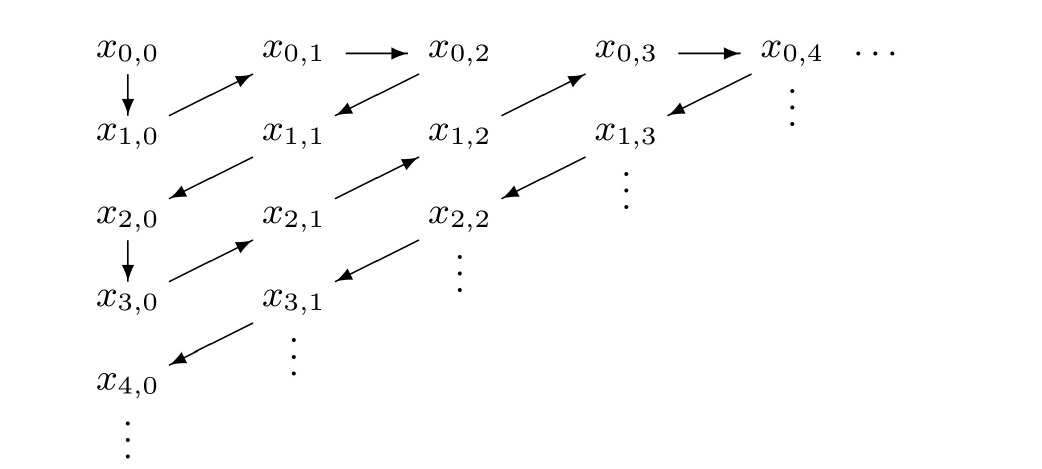
\includegraphics[width=0.78\textwidth]{figures/d1a18a5464e9cd86.jpg}
\end{equation}

我们把明确写出这个双射的任务留给读者。■

\end{proposition}

\begin{proposition}

可数集的有限积是可数的。

\proofhead
设 $X_j, j = 0, 1, \ldots, n$ 是可数集，$X := \prod_{j=0}^{n} X_j$。按定义 $X = (\prod_{j=0}^{n-1} X_j) \times X_n$，故只需考虑 $n = 1$ 的情形。于是设 $X := X_0 \times X_1$，其中 $X_0$ 与 $X_1$ 可数无限。记 $X_0 = \{ y_k : k \in \mathbb{N} \}$，$X_1 = \{ z_k : k \in \mathbb{N} \}$，并对 $j, k \in \mathbb{N}$ 令 $x_{j,k} := (y_j, z_k)$。采用这一记号便有 $X = \{ x_{j,k} : j, k \in \mathbb{N} \}$，因此我们可以再次用 (6.3) 定义从 $X$ 到 $\mathbb{N}$ 的双射。
\end{proposition}

\subsection*{无限积}

若允许可数集的“无限积”，命题 6.9 就不再正确。为使这一说法更精确，我们需要先解释什么是“无限积”。设 $ \{X_\alpha; \alpha \in \mathbb{A}\} $ 是一个固定集合的子集族。则笛卡儿积 $ \prod_{\alpha \in \mathbb{A}} X_\alpha $ 定义为所有这样的函数构成的集合：

$ \varphi: A \to \bigcup_{\alpha \in A} X_\alpha $ 使得对每个 $ \alpha \in A $ 有 $ \varphi(\alpha) \in X_\alpha $。人们常用 $ \{x_\alpha; \alpha \in \mathsf{A}\} $ 代替 $ \varphi $，其中当然 $ x_\alpha := \varphi(\alpha) $。

在特殊情形 $ \mathbf{A} = \{1, \ldots, n\} $（其中 $ n \in \mathbb{N}^\times $）下，$ \prod_{\alpha \in \mathbb{A}} X_\alpha $ 显然与第 2 节引入的积 $ \prod_{k=1}^{n} X_k $ 相同。若对每个 $ \alpha \in \mathbb{A} $ 都有 $ X_\alpha = X $，则记 $ X^{\mathbb{A}} := \prod_{\alpha \in \mathbb{A}} X_\alpha $。

\begin{remark}

显然，若诸 $ X_\alpha $ 中有一个（或更多）是空集，则 $ \prod_{\alpha \in \mathcal{A}} X_\alpha = \emptyset $。另一方面，即使对每个 $ \alpha \in \mathcal{A} $ 都有 $ X_\alpha \neq \emptyset $，用我们迄今所见过的集合论公理也无法证明 $ \prod_{\alpha \in \mathcal{A}} X_\alpha $ 非空。为此需要知道存在函数 $ \varphi: \mathcal{A} \to \bigcup_{\alpha \in \mathcal{A}} X_\alpha $，使得对每个 $ \alpha \in \mathcal{A} $ 有 $ \varphi(\alpha) \in X_\alpha $，即存在一条从每个集合 $ X_\alpha $ 中选出一个元素的规则。为确保这样的函数存在，需要选择公理，我们把它表述如下：对任意集族 $ \{X_\alpha : \alpha \in \mathcal{A}\} $，

\[
\prod_{\alpha\in A}X_{\alpha}\neq\emptyset\Longleftrightarrow(X_{\alpha}\neq\emptyset\;\;\forall\alpha\in\mathsf{A})~.
\]

以下我们将不加说明地使用这一自然出现的公理。对数学基础感兴趣的读者可参阅文献，例如 [Ebb77] 和 [FP85]。■

令人惊讶的是，与命题 6.9 相反，有限集的可数无限积一般不是可数的，如下面的命题所示。

\end{remark}

\begin{proposition}

集合 $ \{0,1\}^{\mathbb{N}} $ 是不可数的。

\proofhead
设 $ A \in \mathcal{P}(\mathbb{N}) $。则特征函数 $ \chi_A $ 是 $ \{0,1\}^{\mathbb{N}} $ 的一个元素。显然函数
\begin{equation}
\mathcal{P}(\mathbb{N})\to\{0,1\}^{\mathbb{N}},\quad A\mapsto\chi_{A}
\end{equation}

是单射。对 $\varphi \in \{0,1\}^{\mathbb{N}}$，令 $A(\varphi):=\varphi^{-1}(1)\in \mathcal{P}(\mathbb{N})$。则 $\chi_{A(\varphi)}=\varphi$。这表明函数 (6.4) 是满射的。（另见习题 3.6。）因此 $\{0,1\}^{\mathbb{N}}$ 与 $\mathcal{P}(\mathbb{N})$ 等势，而结论由推论 6.6 得出。

\end{proposition}

\begin{corollary}

集合 $\{0,1\}^{\mathbb{N}}$ 与 $\mathcal{P}(\mathbb{N})$ 等势。

\end{corollary}

\exerciseshead

\begin{exercises}
\item

设 $ n \in \mathbb{N}^\times $。证明从 $ \{1, \ldots, n\} $ 到自身的任何单射函数都是双射。（提示：对 $ n $ 作归纳。设 $ f: \{1, \ldots, n+1\} \to \{1, \ldots, n+1\} $ 是单射函数，$ k := f(n+1) $。考虑函数

\begin{equation*}
g(j):=\left\{\begin{array}{c l}{n+1\;,}&{\quad j=k\;,}\\ {k\;,}&{\quad j=n+1\;,}\\ {j}&{\quad\text{其他情形},}\\ \end{array}\right.
\end{equation*}

以及 $ h := g \circ f $ 和 $ h | \{1, \ldots, n\} $。）

\item

证明下列各题：

\begin{items}
\item

设 $ m, n \in \mathbb{N}^{\times} $。则存在从 $ \{1, \ldots, m\} $ 到 $ \{1, \ldots, n\} $ 的双射函数当且仅当 $ m = n $。

\item

若 $M$ 是无限系统，则 $\text{Num}(M) = \infty$（提示：习题 1）。

\end{items}

\item

证明 $n$ 元集的 $m$ 元子集的个数是 $\binom{n}{m}$。（提示：设 $N$ 是 $n$ 元集，$M$ 是 $N$ 的 $m$ 元子集。由命题 6.3 推出，有 $m!(n-m)!\; \text{个从} \{1,\ldots,n\} \text{到} N \text{的双射，使得} \{1,\ldots,m\} \text{映到} M.)$

\item

设 M 和 N 是有限集。从 M 到 N 的单射函数有多少个？

\item

设 $ X_0, \ldots, X_m $ 是有限集。证明 $ X := \bigcup_{i=0}^{m} X_j $ 也是有限的，且

\[
Num(X)\leq\sum_{j=0}^{m}Num(X_{j})~.
\]

何时取等号？

\item

设 $ X_0, \ldots, X_m $ 是有限集。证明 $ X := \prod_{i=0}^{m} X_i $ 也是有限的，且

\[
Num(X)=\prod_{j=0}^{m}Num(X_{j})~.
\]
\item

证明非空集合 X 是可数的当且仅当存在从 N 到 X 的满射。

\item

设 $X$ 是可数集。证明 $X$ 的所有有限子集构成的集合是可数的。（提示：考虑函数 $X^n \to \mathcal{E}_n(X)$，$(x_1, \ldots, x_n) \mapsto \{x_1, \ldots, x_n\}$，其中 $\mathcal{E}_n(X)$ 是元素个数至多为 $n$ 的所有子集构成的集合。）

\item

证明有限集的任何子集都是有限的。

\end{exercises}

\section{群与同态}

在定理 5.3 中，当 $ m \leq n $ 时，我们定义了两个自然数 m 与 n 的差 $ n - m $。当 m 是 n 的因子时，我们也定义了两个自然数 m 与 n 的商 n/m。在这两种情形中，对 m 与 n 所加的这些限制都是必需的，以保证差与商仍然是自然数。如果要定义任意自然数 m 与 n 的“差” n - m 或“商” n/m，我们就必须离开自然数的领域。在 9–11 节中，我们将构造新的数，从而把自然数集扩充为更大的数系，在这些数系中这些运算可以（几乎）不受限制地使用。

当然，这些新的数系必须这样构造，使得通常的加法与乘法法则成立。为此，撇开与某一特定数系的联系而考察这些法则本身，是极为有益的。这样的考察也为从定义与公理出发对命题作逻辑推演提供了进一步的练习。

这里以及随后各节所出现问题的深入讨论属于代数而非分析，因此我们的叙述相对简短，只证明少数最重要的定理。我们的目标是能够认出那些以各种伪装反复出现的一般代数结构。从少量公理推导出大量算术法则，将使我们能够为本来庞杂的一堆公式与结果建立秩序，并把注意力保持在本质之处。我们从公理推出的命题，只要公理成立便成立，而与它们成立的具体情境无关。已经证明过一次的东西，无需对每个特殊情形再证明一次。

在本节及随后各节中，我们只给出这些新概念的少数具体例子。我们主要着眼于提供一种语言，并希望读者在后面的各节中能认识到这种语言的用处，同时也能看到形式化背后的数学内容。

\subsection*{群}

群是由一个集合、一个运算和三条公理组成的系统。由于它们具有如此简单的代数结构，因而在数学中处处可见。

由非空集合 G 与一个运算 $ \odot $ 组成的对 $ (G,\odot) $ 称为群，如果下列条件成立：

$ (G_1) $：$ \odot $ 是结合的。

$ (G_{2}) \odot $ 有单位元 e。

$ (G_3) $ 每个 $ g \in G $ 都有一个 $ \mathbf{逆元} $ $ h \in G $，使得 $ g \odot h = h \odot g = e $。

若 $ \odot $ 是 $ G $ 上的交换运算，则群 $ (G, \odot) $ 称为交换群或阿贝尔群。若运算从上下文看是明确的，我们常把 $ (G, \odot) $ 简记为 $ G $。

\begin{remark}

设 $  G = (G, \odot)  $ 是一个群。

\begin{items}
\item

由命题 4.11，单位元 e 是唯一的。

\item

每个 $ g \in G $ 都有唯一的逆元，我们（暂时）把它记为 $ g^b $。特别地 $ e^b = e $。

\proofhead
鉴于 $(G_3)$，只需证明唯一性。设 $h$ 与 $k$ 都是 $g \in G$ 的逆元，即 $g \odot h = h \odot g = e$ 且 $g \odot k = k \odot g = e$。则
\[
h=h\odot e=h\odot(g\odot k)=(h\odot g)\odot k=e\odot k=k,
\]

这就证明了唯一性。
由于 $ e \odot e = e $，第二个断言是显然的。■

\item

对每一对 $a,b\in G$，存在唯一的 $x\in G$ 使 $a\odot x=b$，也存在唯一的 $y\in G$ 使 $y\odot a=b$。也就是说，“方程” $a\odot x=b$ 与 $y\odot a=b$ 有唯一解。

\proofhead
设给定 $a, b \in G$。若令 $x := a^{\flat} \odot b$ 与 $y := b \odot a^{\flat}$，则 $a \odot x = b$ 且 $y \odot a = b$。这证明了存在性。为验证第一个方程解的唯一性，设 $x, z \in G$ 满足 $a \odot x = b$ 且 $a \odot z = b$。则
\[
x=(a^{\flat}\odot a)\odot x=a^{\flat}\odot(a\odot x)=a^{\flat}\odot b=a^{\flat}\odot(a\odot z)=(a^{\flat}\odot a)\odot z=z.
\]

对方程 $ y\odot a=b $ 作类似的论证即完成证明。■

\item

对每个 $ g \in G $，我们有 $ (g^{\flat})^{\flat} = g $。

\proofhead
由逆元的定义直接得到等式
\[
g\odot g^{\flat}=g^{\flat}\odot g=e\;,
\]
\[
\left(g^{\flat}\right)^{\flat}\odot g^{\flat}=g^{\flat}\odot\left(g^{\flat}\right)^{\flat}=e,
\]

它们与 (c) 一起推出 $  g = (g^{\flat})^{\flat}  $。■

\item

设 $H$ 是带有结合运算 $\circledast$ 与单位元 $e$ 的非空集合。若每个元素 $h \in H$ 都有一个 $\text{左} \text{逆} \overline{h}$ 使 $\overline{h} \circledast h = e$，则 $(H, \circledast)$ 是一个群且 $\overline{h} = h^{\flat}$。类似地，若每个元素 $h \in H$ 都有一个 $\text{右} \text{逆} \underline{h}$ 使 $h \circledast \underline{h} = e$，则 $(H, \circledast)$ 是一个群且 $\underline{h} = h^{\flat}$。

\proofhead
设 $h$ 属于 $H$，$\overline{h}$ 是 $h$ 的左逆，且 $\overline{h}$ 是 $\overline{h}$ 的左逆。则 $\overline{\overline{h}} \circledast \overline{h} = e$，于是
\[
h=e\circledast h=\left(\overline{\overline{h}}\circledast\overline{h}\right)\circledast h=\overline{{\overline{{h}}}}~\circledast\left(\overline{{h}}\circledast h\right)=\overline{{\overline{{h}}}}~\circledast e=\overline{{\overline{{h}}}}\;,
\]

由此可得 $ h \circledast \overline{h} = e $。因此 $ \overline{h} $ 也是 $ h $ 的右逆，从而是 $ h $ 的逆。类似地可以证明，若每个元素都有右逆，则每个右逆也是左逆。$ \blacksquare $

\item

对任意的群元素 $ g $ 与 $ h $，$ (g \odot h)^{\flat} = h^{\flat} \odot g^{\flat} $。

\proofhead
由于 $ (h^{\flat}\odot g^{\flat})\odot(g\odot h)=h^{\flat}\odot(g^{\flat}\odot g)\odot h=h^{\flat}\odot e\odot h=h^{\flat}\odot h=e $，该断言由 (e) 推出。■
\end{items}

为了说明一个公理系统是无矛盾的，只需给出某个满足这些公理的数学系统。就群公理 $ (G_{1})-(G_{3}) $ 而言，这相当容易做到，如下面的例子所示。

\end{remark}

\begin{example}

\begin{items}
\item

设 $G := \{e\}$ 是单元素集。则 $\{G, \odot\}$ 是交换群，即\textbf{平凡}群，其（唯一可能的）运算为 $e \odot e = e$。

\item

设 $G := \{a, b\}$ 是带有由右表所定义运算 $\odot$ 的集合。则 $(G, \odot)$ 是交换群。

\item

设 $X$ 是非空集合，$S_X$ 是从 $X$ 到自身的所有双射的集合。当 $\circ$ 表示函数的复合时，$S_X := (S_X, \circ)$ 是一个以 $id_X$ 为单位元的群。此外，反函数 $f^{-1}$ 就是 $f \in S_X$ 在该群中的逆。由习题 4.3，$S_X$ 一般不是交换的。当 $X$ 有限时，$S_X$ 的元素称为置换（见 6 节），$S_X$ 称为 $X$ 的置换群。

\end{items}

\begin{center}
\begin{tabular}{ccc}
\toprule
$ \odot $ & a & b \\
a & a & b \\
b & b & a \\
\bottomrule
\end{tabular}
\end{center}

\begin{items}
\item[（d）]

设 $X$ 是非空集合，$(G, \odot)$ 是一个群。以如例 4.12 中那样的诱导运算 $\odot$，$(G^X, \odot)$ 是一个群。$f \in G^X$ 的逆是函数

\[
f^{\flat}\colon X\to G~,\quad x\mapsto\left(f(x)\right)^{\flat}~.
\]

特别地，当 $ m \geq 2 $ 时，带有运算

\[
(g_{1},\cdots,g_{m})\odot(h_{1},\cdots,h_{m})=(g_{1}\odot h_{1},\cdots,g_{m}\odot h_{m})
\]

的 $ G^m $ 是一个群。

\item[（e）]

设 $ G_1, \ldots, G_m $ 是群。则带有与 (d) 类似地定义的运算的 $ G_1 \times \cdots \times G_m $ 是一个群，称为 $ G_1, \ldots, G_m $ 的直积。■

\end{items}

\end{example}

\subsection*{子群}

设 $ G = (G, \odot) $ 是一个群，$ H $ 是 $ G $ 的非空子集，且对运算 $ \odot $ 封闭，即

$ (\mathrm{SG}_1) $ $ H \odot H \subseteq H $.

若此外还有

(SG$_2$) 对一切 $ h \in H $ 都有 $ h^{\flat} \in H $，

则 $H := (H, \odot)$ 本身也是一个群，称为 $G$ 的子群。这里我们用同一符号 $\odot$ 表示运算在 $H$ 上的限制。由于 $H$ 非空，存在某个 $h \in H$，于是由 $(SG_1)$ 与 $(SG_2)$，$e = h^b \odot h$ 也在 $H$ 中。

\begin{example}

设 $  G = (G, \odot)  $ 是一个群。

\begin{items}
\item

平凡子群 $ \{e\} $ 与 G 本身都是 G 的子群，它们分别是关于包含关系的最小与最大子群（见例 4.4.(b)）。

\item

若 $ H_\alpha $，$ \alpha \in \mathsf{A} $ 是 $ G $ 的子群，则 $ \bigcap_\alpha H_\alpha $ 也是 $ G $ 的子群。■

\end{items}

\end{example}

\subsection*{陪集}

设 $N$ 是 $G$ 的子群，$g \in G$。则 $g \odot N$ 是 $g \in G$ 关于 $N$ 的左陪集，$N \odot g$ 是右陪集。若我们定义

\begin{equation}
g\sim h:\Leftrightarrow g\in h\odot N,
\end{equation}

则 $\sim$ 是 $G$ 上的等价关系：事实上，由于 $e \in N$，$\sim$ 是自反的。若 $g \in h \odot N$ 且 $h \in k \odot N$，则

\[
g\in\left(k\odot N\right)\odot N=k\odot\left(N\odot N\right)=k\odot N~,
\]

因为，当然。

\begin{equation}
N\odot N=N.
\end{equation}

因此 $\sim$ 是传递的。若 $g \in h \odot N$，则存在某个 $n \in N$ 使 $g = h \odot n$。于是由 (SG$_{2}$) 可得 $h = g \odot n^{\flat} \in g \odot N$。因此 $\sim$ 也是对称的，且 (7.1) 定义了 $G$ 上的一个等价关系。对于关于 $\sim$ 的等价类 $[ \cdot ]$，我们有

\begin{equation}
[g]=g\odot N~,\qquad g\in G~.
\end{equation}

因此，我们把 $ G/\sim $ 记为 G/N，并称 G/N 为 G 模 N 的左陪集集合。

特别重要的是满足下式的子群 N：

\begin{equation}
g\odot N=N\odot g~,\qquad g\in G~.
\end{equation}

这样的子群称为 $G$ 的\textbf{正规}子群。此时称 $g\odot N$ 为 $g$ \textbf{模} $N$ 的\textbf{陪集}，因为每个左陪集都是右陪集，反之亦然。

对于 G 的正规子群 N，由 (7.2)、(7.4) 以及运算的结合性可得

\[
(g\odot N)\odot(h\odot N)=g\odot(N\odot h)\odot N=(g\odot h)\odot N~,\qquad g,h,\in G~.
\]

这表明在 $G/N$ 上存在一个由 $\odot$ 诱导的良定义运算，使得

\begin{equation}
(G/N)\times(G/N)\to G/N~,\quad(g\odot N,h\odot N)\mapsto(g\odot h)\odot N~.
\end{equation}

我们将用同一符号 $ \odot $ 表示这个诱导运算。

\begin{proposition}

设 G 是一个群，N 是 G 的正规子群。则带有诱导运算的 G/N 是一个群，称为 G 模 N 的商群。

\proofhead
读者容易验证诱导运算是结合的。由于 $(e\odot N)\odot(g\odot N)=(e\odot g)\odot N=g\odot N$，$G/N$ 的单位元是 $N=e\odot N$。又由于
\[
(g^{\flat}\odot N)\odot(g\odot N)=(g^{\flat}\odot g)\odot N=e\odot N=N
\]

由注 7.1(e) 可得该断言。■

\end{proposition}

\begin{remark}

\begin{items}
\item

在 (7.3) 的记号下，[e] = N 是 $G/N$ 的单位元，$[g]^{\flat}$ = $[g^{\flat}]$ 是 [g] ∈ $G/N$ 的逆元。由 (7.3) 与 (7.5) 我们有

\[
[g]\odot[h]=[g\odot h]~,\qquad g,h\in G~.
\]

换句话说，要用运算 $ \odot $ 合并两个陪集，可以各取每个陪集的一个代表元，用 $ \odot $ 合并这些元素，然后取包含所得元素的陪集。由于 $ G/N $ 上的运算是良定义的，最终结果与代表元的具体选取无关。

\item

阿贝尔群 $G$ 的任何子群 $N$ 都是正规的，因此 $G/N$ 是一个群。当然，$G/N$ 也是阿贝尔群。

\end{items}

\end{remark}

\subsection*{同态}

在群之间的函数中，那些保持群结构的函数特别重要。

设 $ G = (G, \odot) $ 与 $ G' = (G', \circledast) $ 是群。函数 $ \varphi: G \to G' $ 称为（群）同态，如果

\[
\varphi(g\odot h)=\varphi(g)\circledast\varphi(h)~,\qquad g,h\in G~.
\]

从 G 到自身的同态称为（群）自同态。

\begin{remark}

\begin{items}
\item

设 e 与 $ e' $ 分别是 G 与 $ G' $ 的单位元，并设 $ \varphi: G \to G' $ 是一个同态。则

\[
\varphi(e)=e^{\prime}\quad\text{且}\quad\left(\varphi(g)\right)^{\flat}=\varphi(g^{\flat}),\qquad g\in G.
\]

\proofhead
由 $e'\circledast\varphi(e)=\varphi(e)=\varphi(e\odot e)=\varphi(e)\circledast\varphi(e)$ 与注 7.1(c) 可得 $\varphi(e)=e^{\prime}$。设 $g\in G$。则 $e^{\prime}=\varphi(e)=\varphi(g^{\flat}\odot g)=\varphi(g^{\flat})\circledast\varphi(g)$，类似地 $e^{\prime}=\varphi(g)\circledast\varphi(g^{\flat})$。于是由注 7.1(b) 得 $\left(\varphi(g)\right)^{\flat}=\varphi(g^{\flat})$。
\item

设 $ \varphi: G \to G' $ 是一个同态。$ \varphi $ 的核 $ \ker(\varphi) $ 定义为

\[
\ker(\varphi):=\varphi^{-1}(e^{\prime})=\left\{g\in G\;;\;\varphi(g)=e^{\prime}\right\}\;,
\]

是 G 的正规子群。

\proofhead
对一切 $ g, h \in \ker(\varphi) $ 我们有
\[
\varphi(g\odot h)=\varphi(g)\circledast\varphi(h)=e^{\prime}\circledast e^{\prime}=e^{\prime}\;.
\]

因此 (SG$_1$) 满足。由于 $ \varphi(g^{\flat}) = (\varphi(g))^{\flat} = (e')^{\flat} = e' $，(SG$_2$) 也成立，所以 $ \ker(\varphi) $ 是 $ G $ 的子群。设 $ h \in g \odot \ker(\varphi) $。则存在某个 $ n \in G $ 使 $ \varphi(n) = e' $ 且 $ h = g \odot n $。对 $ m := g \odot n \odot g^{\flat} $，我们有

\[
\varphi(m)=\varphi(g)\circledast\varphi(n)\circledast\varphi(g^{\flat})=\varphi(g)\circledast\varphi(g^{\flat})=e^{\prime}~,
\]

从而 $ m \in \ker(\varphi) $。由于 $ m \odot g = g \odot n = h $，这意味着 $ h \in \ker(\varphi) \odot g $。类似地可以证明 $ \ker(\varphi) \odot g \subseteq g \odot \ker(\varphi) $，于是 $ \ker(\varphi) $ 是 $ G $ 的正规子群。$ \blacksquare $

\item

设 $ \varphi: G \to G' $ 是一个同态，$ N := \ker(\varphi) $。则

\[
g\odot N=\varphi^{-1}\bigl(\varphi(g)\bigr),\qquad\quad g\in G,
\]

从而

\[
g\sim h\Longleftrightarrow\varphi(g)=\varphi(h)~,\qquad g,h\in G~,
\]

其中 $ \sim $ 表示等价关系 (7.1)。

\proofhead
对 $ h \in g \odot N $ 我们有
\[
\varphi(h)\in\varphi(g\odot N)=\varphi(g)\circledast\varphi(N)=\varphi(g)\circledast\{e^{\prime}\}=\left\{\varphi(g)\right\},
\]

从而 $ h \in \varphi^{-1}(\varphi(g)) $。反之，若 $ h \in \varphi^{-1}(\varphi(g)) $，即 $ \varphi(h) = \varphi(g) $，则

\[
\varphi(g^{\flat}\odot h)=\varphi(g^{\flat})\circledast\varphi(h)=\left(\varphi(g)\right)^{\flat}\circledast\varphi(g)=e^{\prime}~,
\]

这意味着 $ g^{\flat} \odot h \in N $，从而 $ h \in g \odot N $。■

\item

一个同态是单射当且仅当它的核是平凡的，即 $ \ker(\varphi) = \{e\} $。

\proofhead
这直接由 (c) 推出。
\item

同态 $ \varphi: G \to G' $ 的像 $ \mathrm{im}(\varphi) $ 是 $ G' $ 的子群。■

\end{items}

\end{remark}

\begin{example}

\begin{items}
\item

常值函数 $ G \to G' $，$ g \mapsto e' $ 是同态，即平凡同态。

\item

恒等函数 $ \mathrm{id}_{G}: G \to G $ 是自同态。

\item

同态（自同态）的复合是同态（自同态）。

\item

设 N 是 G 的正规子群。则商函数

\[
p\colon G\to G/N~,\quad g\mapsto g\odot N
\]

是满同态，称为商同态，且 $ \ker(p) = N $。

\proofhead
由于 $N$ 是 $G$ 的正规子群，商群 $G/N$ 是良定义的。由 (7.1) 与命题 4.1，商函数 $p$ 是良定义的，且注 7.5(a) 表明 $p$ 是同态。由于 $N$ 是 $G/N$ 的单位元，$\ker(p)=N$。
\item

若 $ \varphi: G \to G' $ 是双射同态，则 $ \varphi^{-1}: G' \to G $ 也是。■

\end{items}

\end{example}

\subsection*{同构}

若 $\varphi$ 是双射，则同态 $\varphi: G \to G'$ 称为从 $G$ 到 $G'$ 的（群）同构。在此情形下，我们说群 $G$ 与 $G'$ 同构，并记作 $G \cong G'$。从 $G$ 到自身的同构，即双射自同态，称为 $G$ 的（群）自同构。

\begin{example}

\begin{items}
\item

恒等函数 $\mathrm{id}_{G}: G \to G$ 是自同构。若 $\varphi$ 与 $\psi$ 是 $G$ 的自同构，则 $\varphi \circ \psi$ 与 $\varphi^{-1}$ 也是。由此容易推出，群 $G$ 的所有自同构组成的集合以复合为运算构成一个群，称为 $G$ 的自同构群。它是置换群 $S_{G}$ 的子群。

\item

对每个 $ a \in G $，函数 $ g \mapsto a \odot g \odot a^{\flat} $ 是 $ G $ 的自同构。

\item

设 $ \varphi: G \to G' $ 是一个同态。则存在唯一的单射同态 $ \widetilde{\varphi}: G/\ker(\varphi) \to G' $，使得图

\[
\begin{tikzcd}[row sep=2.6em, column sep=3.6em]
G \arrow[r, "\varphi"] \arrow[d, "p"'] & G' \\
G/\ker(\varphi) \arrow[ur, "\widetilde{\varphi}"]
\end{tikzcd}
\]

交换。若 $ \varphi $ 是满射，则 $ \widetilde{\varphi} $ 是同构。

\proofhead
由注 7.6(c) 与例 4.2(c) 可得，存在唯一的单射函数 $ \widetilde{\varphi} $ 使图交换，且 $ \mathrm{im}(\varphi) = \mathrm{im}(\widetilde{\varphi}) $。容易验证 $ \widetilde{\varphi} $ 是同态。
\item

设 $ (G, \odot) $ 是一个群，$ G' $ 是非空集合，$ \varphi: G \to G' $ 是从 $ G $ 到 $ G' $ 的双射。在 $ G' $ 上定义运算 $ \circledast $ 为

\[
g^{\prime}\circledast h^{\prime}:=\varphi^{-1}(g^{\prime})\odot\varphi^{-1}(h^{\prime}),\qquad g^{\prime},h^{\prime}\in G^{\prime}.
\]

则 $ (G', \circledast) $ 是一个群，且 $ \varphi $ 是从 $ G $ 到 $ G' $ 的同构。运算 $ \circledast $ 称为 $ G' $ 上由 $ \varphi $ 从 $ \circledast $ 诱导的运算。

\item

若 $ G = \{e\} $ 与 $ G' = \{e'\} $ 是平凡群，则 G 与 $ G' $ 同构。

\item

设 $G$ 是例 7.2(b) 中的群，$G'$ 是把表中的符号 $a$ 与 $b$ 互换后所得的群。则 $G$ 与 $G'$ 同构。更确切地说，$G'$ 上的运算是由函数 $\varphi: \{a, b\} \to \{a, b\}$（由 $\varphi(a) := b$ 与 $\varphi(b) := a$ 定义）从运算 $G$ 诱导的。

\item

设 X 与 Y 是非空集合，$ \varphi: X \to Y $ 是双射函数。则

\[
\widehat{\varphi}\colon\mathsf{S}_{X}\to\mathsf{S}_{Y}~,\quad f\mapsto\varphi\circ f\circ\varphi^{-1}
\]

是从置换群 $S_X$ 到置换群 $S_Y$ 的同构。■

\end{items}

若 $\varphi$ 是从群 $(G, \odot)$ 到群 $(G', \circ)$ 的同构，那么即使这两个群在元素的记号上可能不同，它们也具有相同的群结构。例如，若 $g$ 与 $h$ 是 $G$ 的两个元素，那么要计算 $g \odot h$，也同样可以在 $G'$ 中计算 $\varphi(g) \otimes \varphi(h)$，然后 $g \odot h$ 就是 $\varphi(g) \otimes \varphi(h)$ 在逆同构 $\varphi^{-1}$ 下的像。实际上，与 $(G', \circ)$ 打交道可能比与 $(G, \odot)$ 容易得多。（特别参见 9 节与 10 节。）

从群论的观点看，同构的群本质上是相同的。事实上，同构 $ \cong $ 是任何群集 $ \mathcal{G} $ 上的等价关系，这容易验证。因此可以用 $ \cong $ 把 $ \mathcal{G} $ 划分为等价类，称为同构类。于是只需研究同构类的集合 $ \mathcal{G}/\cong $，而不必研究 $ \mathcal{G} $ 本身。换句话说，人们把同构的群“等同”（视为相同）。正是在这个意义上，人们谈论平凡群，因为由例 7.8(e)，任何两个平凡群都同构。类似地，阶为\footnote{有限群的阶是其元素的个数。} 2 的群，即恰有两个元素的群，在同构意义下只有一个（见例 7.8(f)）。若 $ n \in \mathbb{N}^\times $，则由例 7.8(g)，只需考虑一个满足 $ \text{Num}(X) = n $ 的置换群 $ S_X $，例如阶为 $ n! $ 的置换群（或对称群），

\[
\mathsf{S}_{n}:=\mathsf{S}_{\{1,\ldots,n\}},
\]

即集合 $ \{1,\ldots,n\} $ 上的置换群。（见命题 6.3。）

约定 在下文中，我们通常把群 $G$ 中的运算记为 $\cdot$，并且对 $x, y \in G$，不写 $x \cdot y$ 而简写为 $xy$。采用这种“乘法”记号时，该运算称为（群）乘法，而 $x^{\flat}$ 写作 $x^{-1}$（“$x$ 的逆”）。若群是阿贝尔群，通常使用“加法记号”，即群运算写作 + 并称为加法，$x$ 的逆 $x^{\flat}$ 写作 $-x$（“负 $x$”）。

再次提醒读者，记号并不重要，重要的是公理。同一符号在不同的

情境中可以具有完全不同的含义，即使适用的公理相同。使用诸如 + 或 $ \cdot $ 这类熟悉的符号，不应使读者以为所指的是熟悉的情境。必须清楚哪些公理在起作用，并只使用由它们推出的规则。

同一个符号可以有各种依赖情境的含义，这在初学者看来也许不合逻辑、令人困惑。尽管如此，它使得复杂思想能够以优雅而简洁的方式得到表述，并避免用大量不同符号使读者不堪重负。

\end{example}

\exerciseshead

\begin{exercises}
\item

设 $N$ 是有限群 $G$ 的子群。证明 $\text{Num}(G) = \text{Num}(N) \cdot \text{Num}(G/N)$，从而特别地，子群的阶整除群的阶。

\item

验证例 7.2(c) 与 (d) 中的断言。

\item

证明例 7.3(b) 中的断言，并证明一组正规子群的交也是正规的。

\item

证明注 7.6(e)。$ \operatorname{im}(\varphi) $ 是 $ G' $ 的正规子群吗？

\item

设 $ \varphi: G \to G' $ 是一个同态，$ N' $ 是 $ G' $ 的正规子群。证明 $ \varphi^{-1}(N') $ 是 G 的正规子群。

\item

设 G 是一个群，X 是非空集合。则称 G（从左）作用在 X 上，若存在一个函数

\[
G\times X\to X~,\quad(g,x)\mapsto g\cdot x
\]

使得下列条件成立：

$ (GA_1)\;e \cdot x = x $ 对一切 $ x \in X $ 成立。

$ (GA_2)\;g\cdot(h\cdot x)=(gh)\cdot x $ 对一切 $ g,h\in G $ 与 $ x\in X $ 成立

\begin{items}
\item

对每个 $g \in G$，证明 $x \mapsto g \cdot x$ 是 $X$ 上的双射，其逆为 $x \mapsto g^{-1} \cdot x$。

\item

对 $ x \in X $，$ G \cdot x $ 称为 $ x $ 的\textbf{轨道}（在 $ G $ 的作用下）。证明关系“$ y $ 在 $ x $ 的轨道中”是 $ X $ 上的等价关系。

\item

证明若 $H$ 是 $G$ 的子群，则 $(h,g) \mapsto h \cdot g$ 与 $(h,g) \mapsto hgh^{-1}$ 定义了 $H$ 在 $G$ 上的作用。

\item

证明

\[
{\sf S}_{m}\times{\mathbb{N}}^{m}\to{\mathbb{N}}^{m},\quad(\sigma,\alpha)\mapsto\sigma\cdot\alpha:=(\alpha_{\sigma(1)},\ldots,\alpha_{\sigma(m)})
\]

定义了 $ S_{m} $ 在 $ N^{m} $ 上的作用。

\end{items}

\item

设 $ G = (G, \odot) $ 是阶为 $ m $、单位元为 $ e $ 的有限群。证明对每个 $ g \in G $，存在最小的自然数 $ k > 0 $ 使得

\[
g^{k}:=\bigodot_{j=1}^{k}g=e.
\]

证明对一切 $ g \in G $ 都有 $ g^m = e $。（提示：习题 1。）

\item

下面的表在集合 $ G = \{e, a, b, c\} $ 上定义了三个运算

\begin{center}
\begin{tabular}{ccccc}
\toprule
$ \odot $ & e & a & b & c \\
e & e & a & b & c \\
a & a & e & c & b \\
b & b & c & e & a \\
c & c & b & a & e \\
\bottomrule
\end{tabular}
\end{center}

\begin{center}
\begin{tabular}{ccccc}
\toprule
$ \circledast $ & e & a & b & c \\
e & e & a & b & c \\
a & a & e & c & b \\
b & b & c & a & e \\
c & c & b & e & a \\
\bottomrule
\end{tabular}
\end{center}

\begin{center}
\begin{tabular}{ccccc}
\toprule
$ \oplus $ & e & a & b & c \\
e & e & a & b & c \\
a & a & b & c & e \\
b & b & c & e & a \\
c & c & e & a & b \\
\bottomrule
\end{tabular}
\end{center}

\begin{items}
\item

验证 $ (G, \circledast) $ 与 $ (G, \oplus) $ 是同构的群。

\item

证明群 $ (G,\odot) $ 与 $ (G,\circledast) $ 不同构。

\item

确定 G 上所有其他可能的群结构。把这些群按同构类分类。

\end{items}

\item

证明 $ S_{3} $ 不是阿贝尔群。

\item

设 G 与 H 是群，并设

\[
p:G\times H\to G~,\quad(g,h)\mapsto g
\]

是到第一个因子的投影。证明 $p$ 是满同态。

令 $H' := \ker(p)$。证明 $(G \times H)/H'$ 与 $G$ 是同构的群。

\item

设 $G$ 是带有运算 $\odot$ 与单位元的集合。对 $g \in G$，定义函数 $Lg: G \to G$，$h \mapsto g \odot h$，称为由 $g$ 给出的左平移。假设

\[
L:=\left\{Lg\;;\;g\in G\right\}\subseteq{\sf S}_{G}~,
\]

即每个 Lg 都是双射。证明

\[
(G,\odot)\text{ 是群 }\Longleftrightarrow L\text{ 是 }\mathsf{S}_{G}\text{ 的子群 }
\]
\end{exercises}

\section{环、域与多项式}

本节我们考虑定义了两种运算的集合。这里我们假定，就其中一种运算而言，该集合构成一个阿贝尔群，并且这两种运算满足适当的“分配律”。由此引出“环”和“域”的概念，它们把算术规则形式化。作为环的特别重要的例子，我们考虑幂级数环以及一个（和多个）未定元的多项式环，并推导它们的一些基本性质。多项式函数相对容易处理，而且在分析中很重要，因为“复杂的函数可以被多项式任意好地逼近”，这一断言我们稍后会说得更精确。

\subsection*{环}

由非空集合  $ R $ 以及两种运算——加法 + 与乘法  $ \cdot $——组成的三元组  $ (R, +, \cdot) $ 称为环，如果：

$ (R_{1}) $  $ (R,+) $ 是阿贝尔群。

(R\_\{2\}) 乘法是结合的。

(R\_\{3\}) 分配律成立：

\[
(a+b)\cdot c=a\cdot c+b\cdot c,\quad c\cdot(a+b)=c\cdot a+c\cdot b,\qquad a,b,c\in R.
\]

这里我们采用通常的约定，即乘法优先于加法。例如， $ a \cdot b + c $ 表示  $ (a \cdot b) + c $（先做乘法  $ d := a \cdot b $，再做加法  $ d + c $），而不是  $ a \cdot (b + c) $。此外，我们通常把  $ a \cdot b $ 写成  $ ab $。

若乘法是交换的，则称一个环为 \textbf{交换环}。此时，分配律  $ (R_{3}) $ 化为

\begin{equation}
(a+b)c=ac+bc~,\qquad a,b,c\in R~.
\end{equation}

若关于乘法存在单位元，则把它记作  $ 1_R $ 或简记为 1，并称为  $ R $ 的单位元（或乘法单位元），此时我们说  $ (R, +, \cdot) $ 是带单位元的环。当加法与乘法运算由上下文清楚可知时，我们只写  $ R $ 而不写  $ (R, +, \cdot) $。

\begin{remark}

设  $ R := (R, +, \cdot) $ 是一个环。

\begin{items}
\item

环  $ R $ 的加法群  $ (R, +) $ 的单位元，如例 5.14 那样记作  $ 0_R $，或简记为 0，并称为环  $ R $ 的零元（或加法单位元）。由命题 4.11， $ 0_R $ 以及  $ 1_R $（若存在）都是唯一的。

\item

由注 7.1(d) 可得，对每个  $ a \in R $ 都有  $ -(-a) = a $。

\item

对每一对 $a, b \in R$，由注 7.1(c)，方程 $a + x = b$ 有唯一解 $x \in R$，即 $x = b + (-a) =: b - a$（“$b$ 减 $a$”），称为 $a$ 与 $b$ 的差。

\item

对一切  $ a \in R $，都有 0a = a0 = 0 与 -0 = 0。若  $ a \neq 0 $ 且存在某个  $ b \neq 0 $ 使 ab = 0 或 ba = 0，则称 a 为 R 的零因子。若 R 是交换环且没有零因子，即由 ab = 0 可推出 a = 0 或 b = 0，则称 R 为整环。

\proofhead
由于 $0=0+0$，我们有 $a0=a(0+0)=a0+a0$。于是由 (c) 与等式 $a0+0=a0$ 可得 $a0=0$。同理可证 $0a=0$。第二个断言也由 (c) 得到。
\item

对一切 $a, b \in R$，都有 $a(-b) = (-a)b = -(ab) =: -ab$ 与 $(-a)(-b) = ab$。

\proofhead
由 $0 = b + (-b)$ 及 (d) 得 $0 = a0 = ab + a(-b)$。因此，正如上面那样，$a(-b) = -ab$。同理可证 $(-a)b = -ab$。两次使用这一事实可得
\[
(-a)(-b)=-\left(a(-b)\right)=-(-ab)=ab,
\]

其中最后一个等号由 (b) 得到。■

\item

若 $R$ 是带单位元的环，则对一切 $a \in R$ 都有 $(-1)a = -a$。

\proofhead
这是 (e) 的特殊情形。■
\item

由例 5.14(a)，对一切  $ n \in \mathbb{N} $ 与  $ a \in R $， $ n \cdot a = na $ 都有定义，且该例中的规则成立。特别地， $ 0_{\mathbb{N}} \cdot a := 0_R $。由 (d) 我们还有  $ 0_R \cdot a := 0_R $，因此略去  $ 0_{\mathbb{N}} $ 与  $ 0_R $ 的下标不会导致歧义。类似地，若  $ R $ 是带单位元的环，则  $ 1_{\mathbb{N}} \cdot a = 1_R \cdot a = a $。

\end{items}

\end{remark}

\begin{example}

\begin{items}
\item

平凡环恰好只有一个元素 0，它本身也记作 0。含有多于一个元素的环称为非平凡的。平凡环显然是交换的，并且有单位元。若 $R$ 是带单位元的环，则由对每个 $a \in R$ 都有 $1_R \cdot a = a$ 可得，$R$ 是平凡的当且仅当 $1_R = 0_R$。

\item

设  $ R := (R, +, \cdot) $ 是环，X 是非空集合。则  $ R^X $ 关于运算

\[
(f+g)(x):=f(x)+g(x)~,\quad(f g)(x):=f(x)g(x)~,\qquad x\in X~,\quad f,g\in R^{X}~.
\]

构成环。若 $R$ 是交换环（带单位元的环），则 $R^X := (R^X, +, \cdot)$ 也是（见例 4.12）。特别地，对 $m \geq 2$，环 $R$ 的直积 $R^m$ 关于运算

\[
(a_{1},\cdots,a_{m})+(b_{1},\cdots,b_{m})=(a_{1}+b_{1},\cdots,a_{m}+b_{m})
\]

以及

\[
(a_{1},\ldots,a_{m})(b_{1},\ldots,b_{m})=(a_{1}b_{1},\ldots,a_{m}b_{m})
\]

构成一个环，称为积环。若 $R$ 是非平凡的带单位元的环，且 $X$ 至少含有两个元素，则 $R^X$ 有零因子。

\proofhead
第一个断言见例 4.12。对第二个断言，设  $ x, y \in X $ 满足  $ x \neq y $，而  $ f, g \in R^X $ 满足  $ f(x) = 1 $ 以及对一切  $ x' \in X \setminus \{x\} $ 有  $ f(x') = 0 $，又满足  $ g(y) = 1 $ 以及对一切  $ y' \in X \setminus \{y\} $ 有  $ g(y') = 0 $。则  $ fg = 0 $。
\item

设 R 是环，S 是 R 的非空子集，且满足以下条件：
 $ (SR_{1}) $ S 是  $ (R, +) $ 的子群。

\[
(\mathrm{S R}_{2})\setminus S\cdot S\subseteq S.
\]

则 $S$ 本身是一个环，即 $R$ 的子环，而 $R$ 称为 $S$ 的扩环。显然，$0 = \{0\}$ 与 $R$ 都是 $R$ 的子环。即使 $R$ 是带单位元的环，$S$ 也未必如此（见 (e)）。即便如此，若 $1_R \in S$，则 $1_R$ 是 $S$ 的单位元。当然，若 $R$ 是交换环，则 $S$ 也是。反之一般不成立。

\item

子环的交是子环。

\item

设  $ R $ 是非平凡的带单位元的环， $ S $ 是所有这样的  $ g \in R^{\mathbb{N}} $ 的集合：对 \textbf{几乎} 所有（即除有限多个之外的一切） $ n \in \mathbb{N} $ 都有  $ g(n) = 0 $。则  $ S $ 是  $ R^{\mathbb{N}} $ 的无单位元的子环。（为什么？）

\item

设 $X$ 是一个集合。对 $X$ 的子集 $A$ 与 $B$，用下式定义它们的对称差 $A \triangle B$：

\[
A\triangle B:=(A\cup B)\backslash(A\cap B)=(A\backslash B)\cup(B\backslash A).
\]

则  $ (\mathcal{P}(X), \triangle, \cap) $ 是带单位元的交换环。■

\end{items}

设 $R$ 与 $R'$ 是环。一个（环）同态是函数 $\varphi: R \to R'$，它与环的运算相容，即

\begin{equation}
\varphi(a+b)=\varphi(a)+\varphi(b)~,\quad\varphi(ab)=\varphi(a)\varphi(b)~,\qquad a,b\in R~.
\end{equation}

此外，若  $ \varphi $ 是双射，则称  $ \varphi $ 为（环）同构，并称 R 与  $ R' $ 同构。

从  $ R $ 到自身的同态  $ \varphi $ 称为（环）自同态。若  $ \varphi $ 是同构，则称它为（环）自同构。\footnote{当上下文清楚地表明所指的是哪一类同态——群、环（以及后来的域、向量空间或代数）——时，我们将使用“同态”“同构”“自同态”等词。}

\end{example}

\begin{remark}

\begin{items}
\item

环同态  $ \varphi: R \to R' $ 特别地是从  $ (R, +) $ 到  $ (R', +) $ 的群同态。 $ \varphi $ 的核  $ \ker(\varphi) $ 定义为这个群同态的核，即

\[
\ker(\varphi)=\left\{a\in R;\;\varphi(a)=0\right\}=\varphi^{-1}(0).
\]
\item

零函数  $ R \to R' $， $ a \mapsto 0_{R'} $ 是同态，且  $ \ker(\varphi) = R $。

\item

设 $R$ 与 $R'$ 是带单位元的环，$\varphi: R \to R'$ 是同态。如 (b) 所示，不能推出 $\varphi(1_R) = 1_{R'}$。这可看作下述事实的结果：就乘法而言，环不是群。

\end{items}

\end{remark}

\subsection*{二项式定理}

下面我们说明，环公理  $ (R_1)-(R_3) $ 除注 8.1 中的规则外还有其他重要的推论。

\begin{theorem}

（二项式定理） 设 $a$ 与 $b$ 是带单位元的环 $R$ 中两个可交换的元素（即 $ab = ba$）。则对一切 $n \in \mathbb{N}$，

\begin{equation}
(a+b)^{n}=\sum_{k=0}^{n}\binom{n}{k}a^{k}b^{n-k}.
\end{equation}

\proofhead
首先我们注意到，由例 5.14、注 8.1(g) 与习题 5.5，(8.3) 的两端都有定义，且该断言对 $n = 0$ 成立。若 (8.3) 对某个 $n \in \mathbb{N}$ 成立，则
\begin{equation*}
\begin{aligned}
(a+b)^{n+1}&=(a+b)^{n}(a+b)=\biggl(\sum_{k=0}^{n}\binom{n}{k}a^{k} b^{n-k}\biggr)(a+b)\\&=\sum_{k=0}^{n}\binom{n}{k}a^{k+1}b^{n-k}+\sum_{k=0}^{n}\binom{n}{k}a^{k} b^{n+1-k}\\&=a^{n+1}+\sum_{k=0}^{n-1}\binom{n}{k}a^{k+1}b^{n-k}+\sum_{k=1}^{n}\binom{n}{k}a^{k} b^{n+1-k}+b^{n+1}\\&=a^{n+1}+\sum_{k=1}^{n}\biggl\{\binom{n}{k-1}+\binom{n}{k}\biggr\}a^{k} b^{n+1-k}+b^{n+1}.
\end{aligned}
\end{equation*}

由习题 5.5 有  $ \binom{n}{k-1}+\binom{n}{k}=\binom{n+1}{k} $，于是

\[
(a+b)^{n+1}=a^{n+1}+\sum_{k=1}^{n}\binom{n+1}{k}a^{k}b^{n+1-k}+b^{n+1}.
\]

于是由命题 5.7 的归纳原理可得该断言。■

\end{theorem}

\subsection*{多项式定理}

我们希望推广二项式定理，使 (8.3) 的左端允许出现多于两项的和。为使这一公式尽可能简单，引入以下记号是有用的：

对满足  $ m \geq 2 $ 的  $ m \in \mathbb{N} $，元素  $ \alpha = (\alpha_1, \ldots, \alpha_m) \in \mathbb{N}^m $ 称为（$ m $ 阶）多重指标。多重指标  $ \alpha \in \mathbb{N}^m $ 的长度  $ |\alpha| $ 由下式定义

\[
|\alpha|:=\sum_{j=1}^{m}\alpha_{j}.
\]

再令

\[
\alpha!:=\prod_{j=1}^{m}(\alpha_{j})!,
\]

并用下式定义  $ \mathbb{N}^{m} $ 上的自然（偏）序

\[
\alpha\leq\beta:\Leftrightarrow(\alpha_{j}\leq\beta_{j},1\leq j\leq m).
\]

最后，设 $R$ 是带单位元的交换环，$m \in \mathbb{N}$ 且 $m \geq 2$。则我们令

\[
a^{\alpha}:=\prod_{j=1}^{m}(a_{j})^{\alpha_{j}}
\]

其中  $ a = (a_1, \ldots, a_m) \in R^m $， $ \alpha = (\alpha_1, \ldots, \alpha_m) \in \mathbb{N}^m $。

\begin{theorem}

（多项式定理） 设 R 是带单位元的交换环。则对一切  $ m \geq 2 $，

\begin{equation}
\Bigl(\sum_{j=1}^{m}a_{j}\Bigr)^{k}=\sum_{|\alpha|=k}\frac{k!}{\alpha!}a^{\alpha}\;,\qquad a=(a_{1},\ldots,a_{m})\in R^{m}\;,\quad k\in\mathbb{N}\;.
\end{equation}

这里  $ \sum_{|\alpha|=k} $ 是对  $ \mathbb{N}^m $ 中一切长度为  $ k $ 的多重指标求和。

\proofhead
我们先对 m 归纳证明
\begin{equation}
k!/\alpha!\in\mathbb{N}^{\times}\qquad\text{对 }k\in\mathbb{N}\text{ 与 }\alpha\in\mathbb{N}^{m}\text{，}|\alpha|=k.
\end{equation}

先考虑  $ m = 2 $ 的情形。设  $ \alpha \in \mathbb{N}^2 $ 是任意一个长度为  $ k $ 的多重指标。则存在某个满足  $ 0 \leq \ell \leq k $ 的  $ \ell \in \mathbb{N} $ 使  $ \alpha = (\ell, k - \ell) $，于是由习题 5.5(b)，

\[
\frac{k!}{\alpha!}=\frac{k!}{\ell!(k-\ell)!}=\binom{k}{\ell}\in\mathbb{N}^{\times}.
\]

现在设 (8.5) 对某个  $ m \geq 2 $ 成立。任取满足  $ |\alpha| = k $ 的  $ \alpha \in \mathbb{N}^{m+1} $。令  $ \alpha' := (\alpha_2, \ldots, \alpha_{m+1}) \in \mathbb{N}^m $。由归纳假设与习题 5.5(a) 可得

\begin{equation}
\frac{k!}{\alpha!}=\frac{(k-\alpha_{1})!}{\alpha^{\prime}!}\binom{k}{\alpha_{1}}\in\mathbb{N}^{\times}.
\end{equation}

这就完成了归纳以及 (8.5) 的证明。

为证明 (8.4)，我们再次对  $ m $ 归纳。 $ m = 2 $ 的情形就是二项式定理。于是我们假设  $ a = (a_1, \ldots, a_m, a_{m+1}) \in R^{m+1} $（对  $ m \geq 2 $）与

 $ k \in \mathbb{N} $ 是给定的。令  $ b := \sum_{j=2}^{m+1} a_j $，并利用定理 8.4 与归纳假设计算如下：

\begin{equation*}
\begin{aligned}
\Big(\sum_{j=1}^{m+1}a_{j}\Big)^{k}=(a_{1}+b)^{k}&=\sum_{\alpha_{1}=0}^{k}\binom{k}{\alpha_{1}}a_{1}^{\alpha_{1}}b^{k-\alpha_{1}}\\&=\sum_{\alpha_{1}=0}^{k}\binom{k}{\alpha_{1}}a_{1}^{\alpha_{1}}\sum_{|\alpha^{\prime}|=k-\alpha_{1}}\frac{(k-\alpha_{1})!}{\alpha^{\prime}!}a_{2}^{\alpha_{2}}\cdot\cdots\cdot a_{m+1}^{\alpha_{m+1}}\\&=\sum_{\alpha_{1}=0}^{k}\sum_{|\alpha^{\prime}|=k-\alpha_{1}}\frac{(k-\alpha_{1})!}{\alpha^{\prime}!}\binom{k}{\alpha_{1}}a_{1}^{\alpha_{1}}\cdot\cdots\cdot a_{m+1}^{\alpha_{m+1}}\\&=\sum_{|\alpha|=k}\frac{k!}{\alpha!}a^{\alpha},
\end{aligned}
\end{equation*}

其中最后一步我们用了 (8.6)。这就完成了归纳以及定理的证明。

\end{theorem}

\begin{remark}

\begin{items}
\item

多项式系数由下式定义\footnote{我们对多项式系数与二项式系数使用同一个符号 $\binom{\cdot}{\cdot}$。这不会引起误解，因为对多项式系数 $\binom{k}{\alpha}$（$k$ 在上、$\alpha$ 在下），有 $\alpha \in \mathbb{N}^m$ 且 $m \geq 2$，而对二项式系数 $\binom{k}{\ell}$（$k$ 在上、$\ell$ 在下），$\ell$ 总是自然数。}

\[
\binom{k}{\alpha}:=\frac{k!}{\alpha!(k-|\alpha|)!}\;,\qquad k\in\mathbb{N}\;,\quad\alpha\in\mathbb{N}^{m}\;,\quad|\alpha|\leq k\;.
\]

则  $ (^k_\alpha) \in \mathbb{N}^\times $，并且若  $ R $ 是带单位元的交换环，则

\[
(1+a_{1}+\cdots+a_{m})^{k}=\sum_{|\alpha|\leq k}{\binom{k}{\alpha}}a^{\alpha}\;,\qquad a=(a_{1},\ldots,a_{m})\in R^{m}\;,\quad k\in\mathbb{N}\;.
\]

\proofhead
若  $ \beta := (\alpha_1, \ldots, \alpha_m, k - |\alpha|) \in \mathbb{N}^{m+1} $，则对一切  $ |\alpha| \leq k $ 都有  $ |\beta| = k $，且  $ \binom{k}{\alpha} = k! / \beta! $。于是由定理 8.5 可得该断言。
\item

显然，若  $ a_1, \ldots, a_m $ 是任意带单位元的环中两两可交换的元素，则定理 8.5 与 (a) 也成立。

\end{items}

\end{remark}

\subsection*{域}

当 $R \setminus \{0\}$ 关于乘法构成群时，环 $R$ 具有特别好的性质。这样的环称为域。具体地说，当下列条件得到满足时，$K$ 是一个域：

(F\_\{1\}) K 是带单位元的交换环。

(F\_\{2\})  $ 0 \neq 1 $。

(F$_3$)  $ K^\times := K \setminus \{0\} $ 关于乘法构成阿贝尔群。

阿贝尔群  $ K^{\times} = (K^{\times}, \cdot) $ 称为 K 的乘法群。

当然，域具有我们已经证明环所具有的一切性质。由于  $ K^{\times} $ 是阿贝尔群，我们同样由注 7.1 得到以下重要规则。

\begin{remark}

设 K 是一个域。

\begin{items}
\item

对一切  $ a \in K^\times $， $ (a^{-1})^{-1} = a $。

\item

域没有零因子。

\proofhead
设  $ ab = 0 $。若  $ a \neq 0 $，则用  $ a^{-1} $ 乘  $ ab = 0 $ 得 b = 0。
\item

设  $ a \in K^\times $ 与  $ b \in K $。则存在唯一的  $ x \in K $ 使  $ ax = b $，即商  $ \frac{b}{a} := b/a := ba^{-1} $（ $ b $ 除以  $ a $）。

\item

对 $a, c \in K$ 与 $b, d \in K^\times$，我们有下列结论：\footnote{用符号 $\pm$ 与 $\mp$ 可以把两个方程写得像一个方程。对其中的一个方程处处用上面的符号（$+$ 或 $-$），对另一个方程则处处用下面的符号。}

\begin{subitems}
\item

$ \frac{a}{b} = \frac{c}{d} \iff ad = bc. $

\item

$ \frac{a}{b} \pm \frac{c}{d} = \frac{ad \pm bc}{bd} $.

\item

$ \frac{a}{b} \cdot \frac{c}{d} = \frac{ac}{bd} $.

\item

$ \frac{a}{b}\bigg/\frac{c}{d} = \frac{ad}{bc},\quad c \neq 0. $

\proofhead
前三个断言可通过把方程两端乘以 bd，再利用由  $ bdx = bdy $ 推出 x = y 这一规则来证明。规则 (iv) 是 (i) 的简单推论。
\end{subitems}

\item

由 (c)，对 $a, b \in K^\times$，方程 $ax = b$ 有唯一解。另一方面，由注 8.1(d)，任何 $x \in K$ 都是方程 $0x = 0$ 的解。这是因为 0 没有乘法逆元。事实上，若 $0^{-1}$ 存在，则会推出 $0 \cdot 0^{-1} = 1$，而由于 $0 \cdot 0^{-1} = 0$，我们就会有 0 = 1，这与 $(F_2)$ 矛盾。这说明零关于乘法所起的特殊作用，它体现在 $K^\times$ 的定义以及“不允许除以零”这一熟悉的观念之中。

\item

设  $ K' $ 是域， $ \varphi: K \to K' $ 是满足  $ \varphi \neq 0 $ 的同态。则

\[
\varphi(1_{K})=1_{K^{\prime}}\quad\text{且}\quad\varphi(a^{-1})=\varphi(a)^{-1}~,\qquad a\in K^{\times}~.
\]

\proofhead
由于  $ \varphi $ 是从  $ K^{\times} $ 到  $ K^{\prime \times} $ 的群同态，这由注 7.6(a) 得到。 $ \blacksquare $
\end{items}

当我们在域的情形使用“同态”“同构”等词时，我们指的当然是“环同态”“环同构”等，而不是群同态。

下面的例子表明域确实存在，因而公理  $ (F_{1})-(\mathrm{F}_{3}) $ 不会导致矛盾。

\end{remark}

\begin{example}

用下表在 \{0,1\} 上定义加法 + 与乘法 ·。

\begin{center}
\begin{tabular}{ccc}
\toprule
+ & 0 & 1 \\
0 & 0 & 1 \\
1 & 1 & 0 \\
\bottomrule
\end{tabular}
\end{center}

\begin{center}
\begin{tabular}{ccc}
\toprule
. & 0 & 1 \\
0 & 0 & 0 \\
1 & 0 & 1 \\
\bottomrule
\end{tabular}
\end{center}

则可以验证  $ \mathbb{F}_2 := (\{0,1\}, +, \cdot) $ 是一个域。事实上，在同构意义下， $ \mathbb{F}_2 $ 是唯一含两个元素的域。 $ \blacksquare $

\end{example}

\subsection*{有序域}

在分析中重要的环与域，通常除代数结构之外还具有序结构。当然，为了证明有趣的定理，人们期望这两种结构以某种方式相容。于是，若带序  $ \leq $ 的环  $ R $ 满足以下条件，则称它为 \textbf{有序环}：\footnote{这里以及下文中，我们写 $a, b, \ldots, w > 0$ 表示 $a > 0, b > 0, \ldots, w > 0$。}

$ (OR_{0}) $  $ (R,\leq) $ 是全序的。

\[
(\mathrm{O R}_{1})~x<y\Rightarrow x+z<y+z,~z\in R.
\]
\[
(\mathrm{OR}_{2})x,y>0\Rightarrow x y>0.
\]

当然，若 x > 0 则称元素  $ x \in R $ 为正的，若 x < 0 则称为负的。我们在下一个命题中汇集有序域的一些简单性质。

\begin{proposition}

设 $ K $ 是有序域，$ x, y, a, b \in K $。

\begin{subitems}
\item

x > y  $ \Leftrightarrow $ x - y > 0.

\item

若 x > y 且 a > b，则  $ x + a > y + b $。

\item

若 a > 0 且 x > y，则 ax > ay。

\item

若 x > 0，则 -x < 0。若 x < 0，则 -x > 0。

\item

设 x > 0。若 y > 0，则 xy > 0。若 y < 0，则 xy < 0。

\item

若 a < 0 且 x > y，则 ax < ay。

\item

对一切  $ x \in K^\times $ 都有  $ x^2 > 0 $。特别地，1 > 0。

\item

若 x > 0，则  $ x^{-1} > 0 $。

\item

若 x > y > 0，则  $ 0 < x^{-1} < y^{-1} $ 且  $ xy^{-1} > 1 $。

\proofhead
所有这些断言都是公理  $ (OR_{1}) $ 与  $ (OR_{2}) $ 的简单推论。我们只验证 (ix) 由 (i)、(viii) 与  $ (OR_{2}) $ 得到，其余证明留给读者。
若 x > y > 0，则 x - y > 0， $ x^{-1} > 0 $ 且  $ y^{-1} > 0 $。由 (OR $ _{2} $) 得
\[
0<(x-y)x^{-1}y^{-1}=y^{-1}-x^{-1},
\]

这蕴含  $ x^{-1} < y^{-1} $，以及

\[
0<(x-y)y^{-1}=x y^{-1}-1,
\]

这蕴含  $ xy^{-1} > 1 $。■

\end{subitems}

\end{proposition}

命题 8.9 的断言 (ii) 与 (vii) 蕴含：例 8.8 中的域 $\mathbb{F}_2$ 不能是有序的，因为否则我们就会有 $0 = 1 + 1 > 0$。在下一节中我们将说明有序域确实存在。

对有序域 $K$，绝对值函数 $|\cdot|: K \to K$ 与符号函数 $\mathrm{sign}(\cdot): K \to K$ 由下式定义

\begin{equation*}
\left|x\right|:=\left\{\begin{array}{r l}{x\quad,\quad}&{x>0\quad,}\\ {0\quad,\quad}&{x=0\quad,}\\ {-x\quad,\quad}&{x<0\quad,}\end{array}\right.\qquad\mathrm{s i g n}x:=\left\{\begin{array}{r l}{1\quad,\quad}&{x>0\quad,}\\ {0\quad,\quad}&{x=0\quad,}\\ {-1\quad,\quad}&{x<0\quad.}\end{array}\right.
\end{equation*}

\begin{proposition}

设 K 是有序域， $ x, y, a, \varepsilon \in K $ 且  $ \varepsilon > 0 $。

\begin{subitems}
\item

$ x = |x| $ sign( $ x $)， $ |x| = x $ sign( $ x $)。

\item

$ |x| = |-x| $， $ x \leq |x| $。

\item

$ |xy| = |x| |y| $.

\item

$ |x| \geq 0 $ 且  $ (|x| = 0 \Leftrightarrow x = 0) $。

\item

$ |x - a| < \varepsilon \Leftrightarrow a - \varepsilon < x < a + \varepsilon $.

\item

$ |x + y| \leq |x| + |y| $（三角不等式）。

\proofhead
前四个断言由定义立即得到。由命题 8.9 的 (vi) 与 (ii) 我们有
\[
|x-a|<\varepsilon\Longleftrightarrow-\varepsilon<x-a<\varepsilon\Longleftrightarrow a-\varepsilon<x<a+\varepsilon,
\]

这就证明了 (v)。为验证 (vi)，先设 $x + y \geq 0$。则由 (ii) 可得 $|x + y| = x + y \leq |x| + |y|$。若 $x + y < 0$，则 $-(x + y) > 0$，因此

\[
|x+y|=|-(x+y)|=|(-x)+(-y)|\leq|-x|+|-y|=|x|+|y|,
\]

这就完成了证明。■

\end{subitems}

\end{proposition}

\begin{corollary}

（反向三角不等式） 在任何有序域 K 中都有

\[
\left|x-y\right|\geq\left|\left|x\right|-\left|y\right|\right|,\qquad x,y\in K.
\]

\proofhead
把三角不等式用于等式  $ x = (x - y) + y $ 得  $ |x| \leq |x - y| + |y| $，即  $ |x| - |y| \leq |x - y| $。在此不等式中交换 x 与 y 得  $ |y| - |x| \leq |y - x| = |x - y| $。■
\end{corollary}

\subsection*{形式幂级数}

设 $R$ 是非平凡的带单位元的环。在集合 $R^{\mathbb{N}} = \mathrm{Funct}(\mathbb{N}, R)$ 上定义加法为

\begin{equation}
(p+q)_{n}:=p_{n}+q_{n}~,\qquad n\in\mathbb{N}~,
\end{equation}

而乘法由卷积定义为

\begin{equation}
(pq)_{n}:=(p\cdot q)_{n}:=\sum_{j=0}^{n} p_{j} q_{n-j}=p_{0}q_{n}+p_{1}q_{n-1}+\cdots+p_{n} q_{0}
\end{equation}

其中 $n \in \mathbb{N}$。这里 $p_n$ 表示 $p \in R^{\mathbb{N}}$ 在 $n \in \mathbb{N}$ 处的值，称为 $p$ 的 $n$ 系数。在这种情形下，元素 $p \in R^{\mathbb{N}}$ 称为 $R$ 上的形式幂级数，并令 $R[[X]] := (R^{\mathbb{N}}, +, \cdot)$。下面的命题表明 $R[[X]]$ 是一个环。注意这个环与例 8.2(b) 中引入的函数环 $R^{\mathbb{N}}$ 不同。

\begin{proposition}

$ R[X] $ 是带单位元的环，即 $ R $ 上的形式幂级数环。若 $ R $ 是交换环，则 $ R[X] $ 也是。

\proofhead
由 (8.7) 与例 7.2(d)， $ (R[X], +) $ 是阿贝尔群。

下面我们证明  $ (R_2) $ 成立。若  $ p, q, r \in R[X] $，则
\begin{equation}
\left((pq)r\right)_{n}=\sum_{j=0}^{n}(pq)_{j}r_{n-j}=\sum_{j=0}^{n}\sum_{k=0}^{j}p_{k}q_{j-k}r_{n-j}
\end{equation}

对一切  $ n \in \mathbb{N} $ 成立。(8.9) 中的二重和是对右图中圆点所对应的所有数对  $ (j, k) $ 求和。由于加法是结合且交换的运算，求和可按任意顺序进行。特别地，求和可以从“先列”改为“先行”，此时 (8.9) 的右端变为

\bookfigure[0.20]{figures/ba38ea330e98fb4a.jpg}
\[
\sum_{k=0}^{n}\sum_{j=k}^{n}p_{k}q_{j-k}r_{n-j}=\sum_{k=0}^{n}p_{k}\sum_{\ell=0}^{n-k}q_{\ell}r_{n-k-\ell}=\sum_{k=0}^{n}p_{k}(qr)_{n-k}=\left(p(qr)\right)_{n},
\]

其中我们令  $ \ell := j - k $。

$(R_3)$ 的成立是清楚的，形式幂级数 $p$（满足 $p_0 = 1$ 且对 $n \in \mathbb{N}^\times$ 有 $p_n = 0$）是 $R[[X]]$ 的单位元这一事实也是清楚的。最后一个断言是平凡的。

我们用 X 表示幂级数

\begin{equation*}
X_{n}:=\left\{\begin{array}{l l}{1,}&{\quad n=1,}\\ {0}&{\quad\text{其他情形}.}\end{array}\right.
\end{equation*}

则对 $X^{m}$ 我们有（见例 5.14(a)）

\begin{equation}
X_{n}^{m}:=\left\{\begin{array}{l l}{1,}&{\quad n=m,}\\ {0,}&{\quad n\neq m,}\\ \end{array}\right.\qquad m,n\in\mathbb{N}.
\end{equation}

特别地， $ X^{0} $ 是 $ R[X] $ 的单位元。

对  $ a \in R $，我们用 $ aX^0 $ 表示常幂级数，

\begin{equation*}
a X_{n}^{0}:=\left\{\begin{array}{l l}{a,}&{\quad n=0,}\\ {0,}&{\quad n>0,}\\ \end{array}\right.
\end{equation*}

而用  $ RX^{0} $ 表示所有常幂级数的集合。由 (8.7) 与 (8.8) 可见， $ RX^{0} $ 是 $ R[X] $ 的包含单位元的子环，且函数

\begin{equation}
R\to R X^{0}~,\quad a\mapsto a X^{0}
\end{equation}

是同构。下面我们通常把 $R$ 与 $RX^0$ 等同，即把常幂级数 $aX^0$ 写成 $a$，并把 $R$ 看作 $R[[X]]$ 的子环。注意 (8.8) 还蕴含

\begin{equation}
(a p)_{n}=a p_{n}~,\qquad n\in\mathbb{N}~,\quad a\in R~,\qquad p\in R[[X]]~.
\end{equation}
\end{proposition}

\subsection*{多项式}

$R$ 上的多项式是形式幂级数 $p \in R[[X]]$，使得 $\{n; p_n \neq 0\}$ 是有限的，换言之，$p_n = 0$ “几乎处处”成立。容易看出，$R[[X]]$ 中所有多项式的集合是 $R[[X]]$ 的包含单位元的子环。这个子环记作 $R[X]$，称为 $R$ 上的多项式环。

若 $p$ 是多项式，则存在某个 $n \in \mathbb{N}$ 使当 $k > n$ 时 $p_k = 0$。由 (8.10) 与 (8.12) 可得 $p$ 可写成形式

\begin{equation}
p=\sum_{k}p_{k}X^{k}=\sum_{k=0}^{n}p_{k}X^{k}=p_{0}+p_{1}X+p_{2}X^{2}+\cdots+p_{n}X^{n}
\end{equation}

其中  $ p_0, \ldots, p_n \in \mathbb{R} $。当然，可能对某些（或全部） $ k \leq n $ 有  $ p_k = 0 $。当多项式按 (8.13) 那样写出时，规则 (8.7) 与 (8.8) 具有形式

\begin{equation}
\sum_{k}p_{k}X^{k}+\sum_{k}q_{k}X^{k}=\sum_{k}(p_{k}+q_{k})X^{k}
\end{equation}

以及

\begin{equation}
\Big(\sum_{k}p_{k}X^{k}\Big)\Big(\sum_{j}q_{j}X^{j}\Big)=\sum_{n}\Big(\sum_{j=0}^{n}p_{j}q_{n-j}\Big)X^{n}.
\end{equation}

注意 (8.15) 可通过把分配律与规则

\[
(a X^{j})(b X^{k})=a b X^{j+k}~,\qquad a,b\in R~,\quad j,k\in\mathbb{N}~,
\]

用于等式左端而得到。

作为  $ R[X] $ 是环这一事实的一个简单应用，我们证明下面的二项式系数加法定理，它推广了习题 5.5 的公式 (ii)。

\qyxffntextdef{1}{这里我们用了这样的事实：两个多项式，即两个从 $\mathbb{N}$ 到 $R$ 的函数，相等当且仅当它们的系数相同。}
\begin{proposition}

对一切  $ \ell, m, n \in \mathbb{N} $，

\[
{\binom{m+n}{\ell}}=\sum_{k=0}^{\ell}{\binom{m}{k}}{\binom{n}{\ell-k}}=\sum_{k=0}^{\ell}{\binom{m}{\ell-k}}{\binom{n}{k}}.
\]

\proofhead
对 $1 + X \in R[X]$，由 (5.15) 可得
\begin{equation}
(1+X)^{m}(1+X)^{n}=(1+X)^{m+n}.
\end{equation}

由于 $X$ 与 $1=1X^{0}=X^{0}$ 可交换，即 $X1=1X$，二项式定理 (8.4) 蕴含

\begin{equation}
(1+X)^{j}=\sum_{i=0}^{j}\binom{j}{i}X^{i}\;,\qquad j\in\mathbb{N}\;.
\end{equation}

于是由 (8.15) 得

\begin{equation*}
\begin{aligned}
(1+X)^{m}(1+X)^{n}=\Big(\sum_{k=0}^{m}\binom{m}{k}X^{k}\Big)\Big(\sum_{j=0}^{n}\binom{n}{j}X^{j}\Big)\\=\sum_{\ell}\Big(\sum_{k=0}^{\ell}\binom{m}{k}\binom{n}{\ell-k}\Big)X^{\ell},
\end{aligned}
\end{equation*}

再由 (8.16) 与 (8.17) 可得

\[
\sum_{\ell}\Bigl(\sum_{k=0}^{\ell}\Bigl(\overset{m}{k}\Bigr)\Bigl(\overset{n}{\ell-k}\Bigr)\Bigr)X^{\ell}=\sum_{\ell}\Bigl(\overset{m+n}{\ell}\Bigr)X^{\ell}~,
\]

这里考虑到了当  $ k > \ell $ 时  $ \binom{\ell}{k} = 0 $。现在通过比较等号两端  $ X^{\ell} $ 的系数即可得到该断言。\qyxffnmark{1} ■

\end{proposition}

若 $p = \sum_k p_k X^k \neq 0$ 是多项式，则由命题 5.5，存在最小的 $m \in \mathbb{N}$ 使当 $k > m$ 时 $p_k = 0$。数 $m$ 称为 $p$ 的 $\text{次数}$，记作 $\text{deg}(p)$，而 $p_m$ 称为 $p$ 的 $\text{首项}\ \text{系数}$。按约定，$\text{零}\ \text{多项式}$ $p = 0$ 的次数为 $-\infty$（$\text{负}\ \text{无穷}$），对此下列关系成立：\footnote{(8.18) 中的约定是为了使 (8.19) 这类法则对零多项式也成立。当然，$-\infty$ 不是自然数，它也不能是某个包含自然数的阿贝尔群的元素。（为什么不能？）}

\begin{equation}
-\infty<k~,\quad k\in\mathbb{N}~,\qquad-\infty+k=k+(-\infty)=-\infty~,\quad k\in\mathbb{N}\cup\{-\infty\}~.
\end{equation}

对  $ k + (-\infty) $ 我们也写作  $ k - \infty $。

显然

\begin{equation}
\deg(p+q)\leq\max\bigl(\deg(p),\deg(q)\bigr),\quad\deg(pq)\leq\deg(p)+\deg(q)
\end{equation}

对一切 $p, q \in R[X]$ 成立。若 $R$ 没有零因子，特别地，若 $R$ 是域，则我们有

\begin{equation}
\deg(pq)=\deg(p)+\deg(q).
\end{equation}

把任意元素  $ p \in R[X] $ 写成如下形式也是方便的

\begin{equation}
p=\sum_{k}p_{k}X^{k}~,
\end{equation}

这解释了“形式幂级数”这一名称。由于“无限和”在  $ R[[X]] $ 中没有意义，这只能看作书写函数  $ p \in R^{\mathbb{N}} $ 的另一种方式。也就是说， $ X^k $ 只是一个占位符，用来表示函数  $ p $ 在  $ k \in \mathbb{N} $ 处取值  $ p_k \in R $。即便如此，关系 (8.14)–(8.15) 仍可用于对这样的无限和进行计算。

\subsection*{多项式函数}

设  $ p = \sum_{k=0}^{n} p_k X^k $ 是 $ R $ 上的多项式。则我们定义 $ p $ 在 $ x \in R $ 处的 \textbf{值} 为

\[
p(x):=\sum_{k=0}^{n}p_{k}x^{k}\in R.
\]

这定义了一个函数

\begin{equation}
\underline{{p}}\colon R\to R~,\quad x\mapsto p(x)~,
\end{equation}

即对应于 $ p \in R[X] $ 的多项式函数 $ \underline{p} \in R^R $。

\begin{remark}

\begin{items}
\item

对应于常多项式 $a$ 的多项式函数是常函数 $(x \mapsto a) \in R^R$。对应于 $X$ 的多项式函数是恒等函数 $\mathrm{id}_R \in R^R$。

\item

设 $R$ 是交换环。则对一切 $p, q \in R[X]$，

\[
(p+q)(x)=p(x)+q(x)~,\quad(p q)(x)=p(x)q(x)~,\qquad x\in R~,
\]

也就是说，函数

\[
R[X]\to R^{R}~,\quad p\mapsto\underline{p}
\]

在  $ R^R $ 具有例 8.2(b) 的环结构时是同态。此外，这个同态把 1 映到 1。

\proofhead
简单的验证留给读者。
\item

若 R 是非平凡的有限环，则函数 (8.22) 不是单射。分析中重要的环是无限的，而对这样的环函数 (8.22) 是单射。

\proofhead
对第一个断言，我们注意到，由于 $R$ 至少有两个元素，由命题 6.7 与 6.11，集合 $R[X] = R^N$ 是不可数的。由于 $R^R$ 是有限集，不可能存在从 $R[X]$ 到 $R^R$ 的单射。第二个断言在注 8.19(d) 中证明。
\item

设 $M$ 是带单位元的环。假设存在函数 $R \times M \to M$，我们把它记作 $(a, m) \mapsto am$。则我们可以定义 $p = \sum_{k=0}^{n} p_k X^k$ 在 $m \in M$ 处的值为

\[
p(m):=\sum_{k=0}^{n} p_{k} m^{k}.
\]

一个平凡但重要的情形是 $R$ 为 $M$ 的子环。此时任何 $p \in R[X]$ 也可看作 $M[X]$ 的元素，因此 $R[X] \subseteq M[X]$。在注 12.12 中我们将回到这一一般情形。

\item

设  $ p = \sum_kp_k X^k \in R[X] $ 是形式幂级数。则对 $ x \in R $ 作形如  $ p(x) := \sum_kp_kx^k $ 的定义是没有意义的，因为“无限和”在  $ R $ 中一般没有定义。即便如此，在 II.9 节中我们将遇到某些形式幂级数，它们具有这样的性质：对某些  $ x \in R $，$ p $ 在 $ x $ 处的值  $ p(x) := \sum_kp_kx^k \in R $ 有意义。

\item

为有效计算 $p(x)$，注意 $p$ 可写成形式

\[
p=\Big(\big(\cdots\big((p_{n}X+p_{n-1})X+p_{n-2}\big)\cdots\big)X+p_{1}\Big)X+p_{0}
\]

（这可用归纳法容易地证明）。这提示了求 $p(x)$ 的一种“迭代过程”：用下式计算 $x_n, x_{n-1}, \ldots, x_0$：

\[
x_{n}:=x~,\quad x_{k-1}:=p_{k}x_{k}+p_{k-1}~,\qquad k=n,n-1,\ldots,1~,
\]

然后令 $p(x)=x_0$。这个“算法”易于编程，且只需 $n$ 次乘法与 $n$ 次加法。另一方面，“直接”计算需要 $2n-1$ 次乘法与 $n$ 次加法。

\end{items}

\end{remark}

\subsection*{多项式的除法}

对域 K 上的多项式，我们现在证明命题 5.4 的带余除法的一个重要版本。

\begin{proposition}

设 $K$ 是域，$p, q \in K[X]$ 且 $q \neq 0$。则存在唯一的多项式 $r$ 与 $s$ 使得

\begin{equation}
p=s q+r\quad\text{ 且 }\quad\deg(r)<\deg(q).
\end{equation}

证明

\begin{items}
\item

存在性：若  $ \deg(p) < \deg(q) $，则  $ s := 0 $ 与  $ r := p $ 满足 (8.23)。于是可设  $ n := \deg(p) \geq \deg(q) =: m $。这样我们有

\[
p=\sum_{k=0}^{n}p_{k}X^{k},\quad q=\sum_{j=0}^{m}q_{j}X^{j},\qquad p_{n}\neq0,\quad q_{m}\neq0.
\]

令 $s_{(1)} := p_n q_m^{-1} X^{n-m} \in K[X]$。则 $p_{(1)} := p - s_{(1)} q$ 是满足 $\deg(p_{(1)}) < \deg(p)$ 的多项式。若 $\deg(p_{(1)}) < m$，则 $s := s_{(1)}$ 与 $r := p_{(1)}$ 满足 (8.23)。否则我们把上述论证用于 $p_{(1)}$ 以代替 $p$。按需重复，经有限多步后我们得到满足 (8.23) 的多项式 $r$ 与 $s$。

\item

唯一性：设 $s_{(1)}$ 与 $r_{(1)}$ 是另外的多项式，具有性质 $p = s_{(1)}q + r_{(1)}$ 与 $\deg(r_{(1)}) < \deg(q)$。则 $(s_{(1)} - s)q = r - r_{(1)}$。若 $s_{(1)} - s \neq 0$，则由 (8.20) 我们会得到

\[
\deg(r-r_{(1)})=\deg\bigl((s_{(1)}-s)q\bigr)=\deg(s_{(1)}-s)+\deg(q)>\deg(q),
\]

而由于  $ \deg(r - r_{(1)}) \leq \max(\deg(r), \deg(r_{(1)})) < \deg(q) $，这是不可能的。因此  $ s_{(1)} = s $，同样  $ r_{(1)} = r $。■

\end{items}

\end{proposition}

注意上述证明是“构造性的”，即多项式 r 与 s 可用 (a) 中描述的方法计算出来。

作为命题 8.15 的第一个应用，我们证明多项式可以按任意  $ a \in K $ “展开”。

\begin{proposition}

设 $K$ 是域，$p \in K[X]$ 是次数为 $n \in \mathbb{N}$ 的多项式，$a \in K$。则存在唯一的 $b_0, b_1, \ldots, b_n \in K$ 使得

\begin{equation}
p=\sum_{k=0}^{n}b_{k}(X-a)^{k}=b_{0}+b_{1}(X-a)+b_{2}(X-a)^{2}+\cdots+b_{n}(X-a)^{n}.
\end{equation}

特别地， $ b_{n} \neq 0 $。

\proofhead
由于  $ \deg(X - a) = 1 $，由命题 8.15 可得存在唯一的  $ p_{(1)} \in K[X] $ 与  $ b_0 \in K $ 使  $ p = (X - a)p_{(1)} + b_0 $。由 (8.20) 我们有  $ \deg(p_{(1)}) = \deg(p) - 1 $，因此该断言可用归纳法证明。
\end{proposition}

\subsection*{一次因式}

命题 (8.16) 的一个直接推论是下面的因式分解定理。

\begin{theorem}

设 $K$ 是域，$p \in K[X]$ 且 $\deg(p) \geq 1$。若 $a \in K$ 是 $p$ 的零点，即 $p(a) = 0$，则 $X - a \in K[X]$ 整除 $p$，即存在唯一的 $q \in K[X]$ 使 $p = (X - a)q$，且 $\deg(q) = \deg(p) - 1$。

\proofhead
把 (8.24) 的两端在 a 处取值得  $ 0 = p(a) = b_{0} $，于是
\[
p=\sum_{k=1}^{n}b_{k}(X-a)^{k}=\Big(\sum_{j=0}^{n-1}b_{j+1}(X-a)^{j}\Big)(X-a),
\]

这就证明了该断言。■

\end{theorem}

\begin{corollary}

域上次数为 m 的非常数多项式至多有 m 个零点。

\end{corollary}

\begin{remark}

设 K 是一个域。

\begin{items}
\item

一般来说，非常数多项式可能没有零点。例如，若 K 是有序域，则由命题 8.9(ii) 与 (vii)，多项式  $ X^{2} + 1 $ 没有零点。

\item

设  $ p \in K[X] $ 且  $ \deg(p) = m \geq 1 $。若  $ a_1, \ldots, a_n \in K $ 是  $ p $ 的全部零点，则  $ p $ 可唯一地写成形式

\[
p=q\prod_{j=1}^{n}(X-a_{j})^{m(j)}
\]

其中  $ q \in K[X] $ 没有零点， $ m(j) \in \mathbb{N}^\times $。这里  $ m(j) $ 称为  $ p $ 的零点  $ a_j $ 的重数。若  $ m(j) = 1 $，则零点  $ a_j $ 是单重的。此外， $ \sum_{j=1}^{n} m(j) \leq m $。

\proofhead
由定理 8.17 用归纳法可得。
\item

若 $p$ 与 $q$ 是 $K$ 上次数 $\leq n$ 的多项式，且对某组互不相同的 $a_1, a_2, \ldots, a_{n+1} \in K$ 有 $p(a_i) = q(a_i)$，则 $p = q$（多项式的恒等定理）。

\proofhead
由 (8.19) 我们有 $\deg(p - q) \leq n$。由于 $p - q$ 有 $n + 1$ 个零点，该断言由推论 8.18 得到。
\item

若 K 是无限域，即集合 K 是无限的，则同态 (8.22) 是单射。\footnote{对有限域，这个论断不成立。见注 8.14(c) 与习题 16。}

\proofhead
若 $p, q \in K[X]$ 满足 $\underline{p} = \underline{q}$，则对一切 $x \in K$ 有 $p(x) = q(x)$。由于 $K$ 是无限的，由 (c) 可得 $p = q$。■
\end{items}

\end{remark}

\subsection*{多元不定元的多项式}

为结束本节，我们把上述结果推广到 $m$ 个未定元的形式幂级数与多项式的情形。与 $m=1$ 的情形（即 $R[[X]]$ 与 $R[X]$）类似，对 $m\in\mathbb{N}^\times$，我们在集合 $R^{(\mathbb{N}^m)}=\mathrm{Funct}(\mathbb{N}^m,R)$ 上定义加法与乘法为

\begin{equation}
(p+q)_{\alpha}:=p_{\alpha}+q_{\alpha}~,\qquad\alpha\in\mathbb{N}^{m}~,
\end{equation}

以及

\begin{equation}
(p q)_{\alpha}:=\sum_{\beta\leq\alpha}p_{\beta}q_{\alpha-\beta}~,\qquad\alpha\in\mathbb{N}^{m}~.
\end{equation}

在 (8.26) 中，求和遍及一切满足  $ \beta \leq \alpha $ 的多重指标  $ \beta \in \mathbb{N}^m $。在这种情形下， $ p \in R^{(\mathbb{N}^m)} $ 称为 $ R $ 上 $ m $ 个未定元的形式幂级数。我们令

\[
R[\left[X_{1},\ldots,X_{m}\right]]:=\left(R^{(\mathbb{N}^{m})},+,\cdot\right),
\]

其中 + 与 · 如 (8.25) 与 (8.26) 中那样。

若形式幂级数  $ p \in R[X_1, \ldots, X_m] $ 对几乎所有的  $ \alpha \in \mathbb{N}^m $ 都有  $ p_\alpha = 0 $，则称它为 $ R $ 上 $ m $ 个未定元的多项式。所有这种多项式的集合记作  $ R[X_1, \ldots, X_m] $。

令  $ X := (X_1, \ldots, X_m) $，并对  $ \alpha \in \mathbb{N}^m $，用  $ X^\alpha $ 表示满足下式的形式幂级数（即函数  $ \mathbb{N}^m \to R $）

\begin{equation*}
X_{\beta}^{\alpha}:=\left\{\begin{array}{l l}{1,}&{\quad\beta=\alpha,}\\ {0,}&{\quad\beta\neq\alpha,}\\ \end{array}\right.\qquad\beta\in\mathbb{N}^{m}.
\end{equation*}

则每个 $p \in R[[X_1,\ldots,X_m]]$ 都可唯一地写成形式

\[
p=\sum_{\alpha\in\mathbb{N}^{m}}p_{\alpha}X^{\alpha}.
\]

规则 (8.25) 与 (8.26) 变为

\begin{equation}
\sum_{\alpha\in\mathbb{N}^{m}}p_{\alpha}X^{\alpha}+\sum_{\alpha\in\mathbb{N}^{m}}q_{\alpha}X^{\alpha}=\sum_{\alpha\in\mathbb{N}^{m}}(p_{\alpha}+q_{\alpha})X^{\alpha}
\end{equation}

以及

\begin{equation}
\Big(\sum_{\alpha\in\mathbb{N}^{m}}p_{\alpha}X^{\alpha}\Big)\Big(\sum_{\beta\in\mathbb{N}^{m}}q_{\beta}X^{\beta}\Big)=\sum_{\alpha\in\mathbb{N}^{m}}\Big(\sum_{\beta\leq\alpha}p_{\beta}q_{\alpha-\beta}\Big)X^{\alpha}\;.
\end{equation}

同样，(8.27) 与 (8.28) 可通过使用分配律与规则

\[
a X^{\alpha}b X^{\beta}=a b X^{\alpha+\beta},\qquad a,b\in R,\quad\alpha,\beta\in\mathbb{N}^{m}.
\]

多项式

\begin{equation}
p=\sum_{\alpha\in\mathbb{N}^{m}}p_{\alpha}X^{\alpha}\in R[X_{1},\ldots,X_{m}]
\end{equation}

的次数由下式定义\footnote{我们约定 $\max(\emptyset) = -\infty$ 与 $\min(\emptyset) = \infty$。}

\[
\mathrm{d e g}(p):=\max\{|\alpha|\in\mathbb{N}\;;\;p_{\alpha}\neq0\}.
\]

形如  $ p_{\alpha}X^{\alpha} $（其中  $ \alpha \in \mathbb{N}^m $）的多项式称为单项式。若只要  $ |\alpha| \neq k $ 就有  $ p_{\alpha} = 0 $，则称多项式 (8.29) 是 $ k $ 次齐次的。每个次数为  $ k \in \mathbb{N} $ 的齐次多项式都具有形式

\[
\sum_{|\alpha|=k}p_{\alpha}X^{\alpha}\;,\qquad p_{\alpha}\in R\;.
\]

次数  $ \leq 0 $ 的多项式称为 $ \text{常数多项式} $，次数为 1 的多项式称为 $ \text{线性多项式} $，次数为 2 的多项式称为 $ \text{二次多项式} $。

\begin{remark}

\begin{items}
\item

$ R[[X_1, \ldots, X_m]] $ 是带单位元  $ X^0 = X^{(0,0,\ldots,0)} $ 的环，即  $ X^0 $ 是函数  $ \mathbb{N}^m \to R $，它在  $ (0, 0, \ldots, 0) $ 处取值 1，在其他处取值为零。若  $ R $ 是交换环，则  $ R[[X_1, \ldots, X_m]] $ 也是。未定元  $ X_1, \ldots, X_n $ 的多项式环，即  $ R[X_1, \ldots, X_n] $，是  $ R[[X_1, \ldots, X_m]] $ 的子环。 $ R $ 同构于  $ R[[X_1, \ldots, X_n]] $ 的子环  $ RX^0 := \{a X^0 : a \in R\} $。借助这个同构我们把  $ R $ 与  $ RX^0 $ 等同，从而把  $ R $ 看作  $ R[X_1, \ldots, X_n] $ 的子环，并把  $ a X^0 $ 写成  $ a $。

\item

设 $R$ 是交换环，$p \in R[X_1, \ldots, X_m]$。则我们定义 $p$ 在 $x := (x_1, \ldots, x_m) \in R^m$ 处的值为

\[
p(x):=\sum_{\alpha\in\mathbb{N}^{m}}p_{\alpha}x^{\alpha}\in R,
\]

并定义相应的（m 元）多项式函数为

\[
\underline{p}:R^{m}\to R~,\quad x\mapsto p(x)~.
\]

函数

\begin{equation}
R[X_{1},\ldots,X_{m}]\to R^{(R^{m})}~,\quad p\mapsto\underline{p}
\end{equation}

在  $ R^{(R^{m})} $ 被赋予例 8.2(b) 的环结构时是同态。

\item

设 K 是无限域。则同态 (8.30) 是单射。

\proofhead
设 $p \in K[X_1, \ldots, X_m]$。则由注 7.6(d)，只需证明：若对一切 $x = (x_1, \ldots, x_m) \in K^m$ 都有 $\underline{p}(x) = 0$，则 $\underline{p}$ 为零。显然 $p = \sum_\alpha p_\alpha X^\alpha$ 可写成形式
\begin{equation}
p=\sum_{j=0}^{n}q_{j} X_{m}^{j}
\end{equation}

其中  $ n \in \mathbb{N} $ 与  $ q_j \in K[X_1, \ldots, X_{m-1}] $ 适当选取。这提示了对未定元个数作归纳的证明：对  $ m = 1 $，由注 8.19(d) 该断言成立。下面设该断言对  $ 1 \leq k \leq m-1 $ 成立。利用 (8.31)，令

\[
p_{(x^{\prime})}:=\sum_{j=0}^{n}\underline{{q}}_{j}(x_{1},\ldots,x_{m-1})X^{j}\in K[X]~,\qquad x^{\prime}:=(x_{1},\ldots,x_{m-1})\in K^{m-1}~.
\]

由于对  $ x \in K^{m} $ 有  $ \underline{p}(x) = 0 $，故对每个  $ \xi \in K $ 与固定的  $ x^{\prime} \in K^{m-1} $ 都有  $ p_{(x^{\prime})}(\xi) = 0 $。
注 8.19(d) 蕴含  $ p_{(x^{\prime})} = 0 $，即对一切  $ 0 \leq j \leq n $ 都有  $ \underline{q}_{j}(x_{1}, \ldots, x_{m-1}) = 0 $。由于  $ x^{\prime} \in K^{m-1} $ 是任意的，由归纳法可得对一切  $ j = 0, \ldots, n $ 都有  $ q_{j}(X_{1}, \ldots, X_{m-1}) = 0 $。这当然蕴含  $ p = 0 $。■

\end{items}

约定 设 $K$ 是无限域，$m \in \mathbb{N}^\times$。则我们把多项式环 $K[X_1, \ldots, X_m]$ 与它在 $K^{(K^m)}$ 中在同态 (8.30) 下的像等同。换句话说，我们把多项式 $p \in K[X_1, \ldots, X_m]$ 与多项式函数

\[
K^{m}\to K~,\quad x\mapsto p(x)~.
\]

等同。因此  $ K[X_1, \ldots, X_m] $ 是  $ K^{(K^m)} $ 的子环，我们称它为 $ R $ 上 $ m $ 个未定元的多项式环。

\end{remark}

\exerciseshead

\begin{exercises}
\item

设 $a$ 与 $b$ 是带单位元的环中可交换的元素，$n \in \mathbb{N}$。

证明以下结论：

\begin{items}
\item

$ a^{n+1} - b^{n+1} = (a - b) \sum_{j=0}^{n} a^j b^{n-j} $.

\item

$ a^{n+1} - 1 = (a - 1) \sum_{j=0}^{n} a^j $.
注  $ \sum_{j=0}^{n} a^{j} $ 称为 $ R $ 中的有限几何级数。

\end{items}

\item

对带单位元的环  $ R $，证明在  $ R[X] $ 中  $ (1 - X) \sum_k X^k = (\sum_k X^k)(1 - X) = 1 $。

注  $ \sum_k X^k $ 称为几何级数。

\item

证明域上一个未定元的多项式环没有零因子。

\item

证明有限域不能是有序的。

\item

证明注 8.20(a) 与 (b)。

\item

设 R 是带单位元的环。若 RI = IR = I，则称子环 I 为 R 的理想。若理想是 R 的真子集，则称它为真理想。证明以下结论：

\begin{items}
\item

理想 $I$ 是真理想当且仅当 $1 \notin I$。

\item

域 K 恰好有两个理想： $ \{0\} $ 与 K。

\item

若  $ \varphi: R \to R' $ 是环同态，则  $ \ker(\varphi) $ 是 R 的理想。

\item

一族理想的交是理想。

\item

设 I 是 R 的理想，并设 R/I 是商群  $ (R, +)/I $。在 R/I 上定义运算

\[
R/I\times R/I\to R/I~,\quad(a+I,b+I)\mapsto a b+I~.
\]

证明以这个运算作为乘法时， $ R/I $ 是一个环，且商同态  $ p: R \to R/I $ 是环同态。
注 $R/I$ 称为 $R$ 模 $I$ 的商环，而对 $a \in R$，$a + I$ 是 $a$ 模 $I$ 的陪集。我们常把 $a \in b + I$ 写成 $a \equiv b$ (mod $I$)（‘$a$ 同余于 $b$ 模 $I$’）。

\end{items}

\item

设 $R$ 是带单位元的交换环，$m \in \mathbb{N}$ 且 $m \geq 2$。设

\[
\mathsf{S}_{m}\times\mathbb{N}^{m}\to\mathbb{N}^{m},\quad(\sigma,\alpha)\mapsto\sigma\cdot\alpha
\]

是如习题 7.6(d) 中那样的对称群  $ S_m $ 在  $ N^m $ 上的作用。证明以下结论：

\begin{items}
\item

等式

\[
\sigma\cdot\textstyle\sum_{\alpha}a_{\alpha}X^{\alpha}:=\sum_{\alpha}a_{\alpha}X^{\sigma\cdot\alpha}
\]

定义了一个作用

\[
\mathsf{S}_{m}\times R[X_{1},\ldots,X_{m}]\to R[X_{1},\ldots,X_{m}]~,\quad(\sigma,p)\mapsto\sigma\cdot p
\]

f Sm 在多项式环  $ R[X_1,\ldots,X_m] $ 上。

\item

对每个  $ \sigma \in \mathcal{S}_m $， $ p \mapsto \sigma \cdot p $ 是  $ R[X_1, \ldots, X_m] $ 的自同构。

\item

确定下列情形中的轨道  $ S_{3} \cdot p $：

\begin{subitems}
\item

p := X\_\{1\}.

\item

p :=  $ X_{1}^{2} $.

\item

$ p := X_1^2 X_2 X_3^3 $.

\end{subitems}

\item

若  $ \mathbf{S}_m \cdot p = \{p\} $，即它被所有置换固定，则称多项式  $ p \in R[X_1, \ldots, X_m] $ 为 \textbf{对称的}。证明  $ p $ 是对称的当且仅当它具有形式

\[
p=\sum_{[\alpha]\in\mathbb{N}^{m}/\mathbb{S}_{m}}a_{[\alpha]}\left(\sum_{\beta\in[\alpha]}X^{\beta}\right)
\]

其中对一切  $ [\alpha] \in \mathbb{N}^{m} / \mathbb{S}_{m} $ 都有  $ a_{[\alpha]} \in R $。

\item

确定 3 个未定元中一切次数  $ \leq 3 $ 的对称多项式。

\item

证明初等对称函数

\begin{equation*}
\begin{aligned}
s_{1}&:=\sum_{1\leq j\leq m}X_{j}\\s_{2}&:=\sum_{1\leq j<k\leq m}X_{j}\cdot X_{k}\\&\vdots\\s_{k}&:=\sum_{1\leq j_{1}<j_{2}<\cdots<j_{k}\leq m}X_{j_{1}}\cdot X_{j_{2}}\cdot\cdots\cdot X_{j_{k}}\\&\vdots\\s_{m}&:=X_{1}X_{2}\cdots X_{m}
\end{aligned}
\end{equation*}

是对称多项式。

\item

证明多项式

\[
(X-X_{1})(X-X_{2})\cdots(X-X_{m})\in R[X_{1},\ldots,X_{m}][X]
\]

即环  $ R[X_1,\ldots,X_m] $ 上一个未定元 X 的多项式，满足

\[
(X-X_{1})(X-X_{2})\cdots(X-X_{m})=\sum_{k=0}^{m}(-1)^{k}s_{k}X^{m-k}
\]

其中  $ s_0 := 1 \in \mathbb{R} $。

\end{items}

\item

设 $R$ 是带单位元的交换环。对 $r \in R$，用 $p[r] := \sum_k r^k X^k$ 定义幂级数 $p[r] \in R[[X]]$。证明以下结论：

\begin{items}
\item

$ (p[1])^m = \sum_k \binom{m+k-1}{k} X^k $,  $ m \in \mathbb{N}^\times $.

\[
\prod_{j=1}^{m}p[a_{j}]=\sum_{k}\big(\sum_{|\alpha|=k}a^{\alpha}\big)X^{k},~a:=(a_{1},\ldots,a_{m})\in R^{m},~m\in\mathbb{N}\text{ 满足 }m\geq2.
\]
\end{items}

\begin{items}
\item[（c）]

$ \sum_{\substack{\alpha \in \mathbb{N}^m \\ |\alpha| = k}} 1 = \binom{m + k - 1}{k} $.

\item[（d）]

$ \sum_{\substack{\alpha \in \mathbb{N}^m \\ |\alpha| \leq k}} 1 = \binom{m + k}{k} $.

\end{items}

\item

验证对任意集合 $X$，$(\mathcal{P}(X), \triangle, \cap)$ 是带单位元的交换环（见例 8.2(f)）。

\item

设 K 是有序域， $ a, b, c, d \in K $。

\begin{items}
\item

证明不等式  $ \frac{|a+b|}{1+|a+b|} \leq \frac{|a|}{1+|a|} + \frac{|b|}{1+|b|} $。

\item

证明：若 $b > 0$，$d > 0$ 且 $\frac{a}{b} < \frac{c}{d}$，则 $\frac{a}{b} < \frac{a+c}{b+d} < \frac{c}{d}$。

\item

证明：若 $a, b \in K^\times$，则 $\left|\frac{a}{b} + \frac{b}{a}\right| \geq 2$。

\end{items}

\item

证明在任何有序域 K 中都有

\begin{equation*}
\sup\{a,b\}=\max\{a,b\}=\frac{a+b+\left|a-b\right|}{2}\ ,\qquad\begin{array}{l}a,b\in K.\end{array}
\end{equation*}
\[
\inf\{a,b\}=\min\{a,b\}=\frac{a+b-|a-b|}{2},
\]
\item

设  $ R $ 是有序环， $ a, b \in R $ 满足  $ a \geq 0 $ 与  $ b \geq 0 $。假设存在某个  $ n \in \mathbb{N}^\times $ 使  $ a^n = b^n $。证明  $ a = b $。

\item

证明例 8.2(d) 与 (e) 中的断言。

\item

设  $ K $ 是域。对  $ p = \sum_{k=0}^{n} p_k X^k \in K[X] $，令

\[
D p:=\sum_{k=1}^{n}k p_{k}X^{k-1}\in K[X],
\]

若  $ n \in \mathbb{N}^\times $；若  $ p $ 是常数，则  $ Dp = 0 $。证明

\[
D(p q)=p D q+q D p~,\qquad p,q\in K[X]~.
\]
\item

求满足  $ \deg(r) < 3 $ 的  $ r, s \in K[X] $，使得

\[
X^{5}-3X^{4}+4X^{3}=s(X^{3}-X^{2}+X-1)+r.
\]
\item

设 K 是有限域。证明同态

\[
K[X]\to K^{K}~,\quad p\mapsto\underline{p}
\]

由注 8.14(b) 给出，它一般不是单射。（提示： $ p := X^2 - X \in \mathbb{F}_2[X] $。）

\end{exercises}

\section{有理数}

在前两节的代数考察之后，我们回到最初关于把自然数扩充为更大数系的问题。我们希望这样的扩充保持自然数通常的交换律、结合律与分配律。此外，元素的任意差与（几乎任意的）商都应当存在。鉴于注 8.1 与 8.7，这些所期望的性质刻画了域，因此更精确的目标是把 $ \mathbb{N} $“嵌入”一个域中，使得域运算限制到 $ \mathbb{N} $ 上时与定理 5.3 中所见的自然数的通常加法与乘法一致。由于 N 具有一个与运算 + 和 - 相容的全序，我们期待这种序结构也应当扩展到整个域。定理 5.3 表明，至少用自然数进行计算的法则与有序域中出现的法则并不矛盾。我们将在本节看到，我们的问题本质上只有唯一的答案。为此，我们首先把 N 嵌入整数环，然后再把这个环扩展为有理数域。

\subsection*{整数}

由定理 5.3 可见，$ \mathbb{N} = (\mathbb{N}, +, \cdot) $ “几乎”是一个有单位元的交换环。唯一缺少的性质是每个 $ n \in \mathbb{N} $ 都存在加法逆元 $ -n $。

设 $Z$ 是一个包含 $\mathbb{N}$ 的环，且 $Z$ 上的环运算限制到 $\mathbb{N}$ 上就是通常的运算。则对所有 $(m, n) \in \mathbb{N}^2$，差 $m - n$ 是 $Z$ 中一个定义明确的元素，并且

\begin{equation}
m-n=m^{\prime}-n^{\prime}\Longleftrightarrow m+n^{\prime}=m^{\prime}+n~,\qquad(m^{\prime},n^{\prime})\in\mathbb{N}^{2}~.
\end{equation}

对于两个这样的元素之和，我们有

\begin{equation}
(m-n)+(m^{\prime}-n^{\prime})=(m+m^{\prime})-(n+n^{\prime})~,
\end{equation}

而它们的积为

\begin{equation}
(m-n)\cdot(m^{\prime}-n^{\prime})=(mm^{\prime}+nn^{\prime})-(mn^{\prime}+m^{\prime}n).
\end{equation}

注意到每个方程右端括号中的加法与乘法可以完全在 $ \mathbb{N} $ 内进行。这一观察提示我们用 $ (9.2) $ 与 $ (9.3) $ 在 $ (m, n) \in \mathbb{N}^2 $ 上定义加法与乘法。这样做时我们不应忽视 $ (9.1) $，它表明两对不同的自然数可能对应于我们正在构造的环中的同一个元素。下面的定理表明这一策略是成功的。

\begin{theorem}

存在一个有单位元的最小整环（无零因子的交换环）$\mathbb{Z}$，使得 $\mathbb{N} \subseteq \mathbb{Z}$ 且 $\mathbb{Z}$ 上的环运算限制到 $\mathbb{N}$ 上就是通常的运算。这个环在同构意义下唯一，称为整数环。

\proofhead
我们只概述证明中最重要的步骤，而把运算定义明确以及环公理 $ (R_1)-(R_3) $ 得到满足这些容易的验证留给读者。

在 $ \mathbb{N}^{2} $ 上由下式定义等价关系
\[
(m,n)\sim(m^{\prime},n^{\prime}):\Longleftrightarrow m+n^{\prime}=m^{\prime}+n,
\]

并令 $ \mathbb{Z} := \mathbb{N}^2 / \sim $。由下式在 $ \mathbb{Z} $ 上定义加法与乘法

\[
[(m,n)]+[(m^{\prime},n^{\prime})]:=[(m+m^{\prime},n+n^{\prime})]
\]

以及

\[
[(m,n)]\cdot[(m^{\prime},n^{\prime})]:=[(m m^{\prime}+n n^{\prime},m n^{\prime}+m^{\prime}n)]~.
\]

定理 5.3 中 $ \mathbb{N} $ 的算术法则蕴含 $ \mathbb{Z} := (\mathbb{Z}, +, \cdot) $ 是一个无零因子的交换环。$ \mathbb{Z} $ 的零元与单位元分别是等价类 $ [(0, 0)] $ 与 $ [(1, 0)] $。

函数

\begin{equation}
\mathbb{N}\to\mathbb{Z}~,\quad m\mapsto\left[(m,0)\right]
\end{equation}

是单射，且与 $ \mathbb{N} $ 和 $ \mathbb{Z} $ 中的加法与乘法运算相容。因此，我们可以把 $ \mathbb{N} $ 与它在 (9.4) 下的像等同起来。于是 $ \mathbb{N} \subseteq \mathbb{Z} $，且 $ \mathbb{Z} $ 上的运算限制到 $ \mathbb{N} $ 上就是通常的运算。

现在设 $ R \supseteq \mathbb{N} $ 是某个有单位元且无零因子的交换环，使得 $ R $ 上的运算限制到 $ \mathbb{N} $ 上就是通常的运算。由于按构造 $ \mathbb{Z} $ 显然是最小的，故存在唯一的单射同态 $ \varphi: \mathbb{Z} \to R $，满足 $ \varphi | \mathbb{N} = (\mathbb{N} \text{ 到 } R \text{ 的包含映射}) $。这蕴含了所说的同构意义下的唯一性。

下文我们不再区分 $ \mathbb{Z} $ 的不同同构副本，而说（唯一的）$ \mathbf{整数环} $。（另一种做法：一次性固定 $ \mathbb{Z} $ 的同构类的一个特定代表，并称之为 $ \mathbf{整数环} $。）$ \mathbb{Z} $ 的元素是 $ \mathbf{整数} $，而 $ -\mathbb{N}^\times := \{-n; n \in \mathbb{N}^\times\} $ 是 $ \mathbf{负整数} $ 的集合。显然 $ \mathbb{Z} = \mathbb{N}^\times \cup \{0\} \cup (-\mathbb{N}^\times) = \mathbb{N} \cup (-\mathbb{N}^\times) $ 是不交并。

\end{theorem}

\subsection*{有理数}

在环 $ \mathbb{Z} $ 中，我们现在可以作任意的差 $ m - n $，但一般来说，两个整数的商 $ m/n $ 仍未定义，即使 $ n \neq 0 $。例如，方程 $ 2x = 1 $ 在 $ \mathbb{Z} $ 中无解，因为若 $ 2(m - n) = 1 $ 且 $ m, n \in \mathbb{N} $，则 $ 2m = 2n + 1 $，这与命题 5.4 矛盾。为克服这一“缺陷”，我们将构造一个包含 $ \mathbb{Z} $ 作为子环的域 $ K $。当然，我们取 $ K $ “尽可能小”。

按照把 $ \mathbb{N} $ 扩充到 $ \mathbb{Z} $ 时确立的模式，我们首先假设 $ K $ 是这样一个域。于是，对于 $ a, c \in \mathbb{Z} $ 与 $ b, d \in \mathbb{Z}^\times := \mathbb{Z} \setminus \{0\} $，我们有注 8.7(d) 中的关系 (i)。这提示我们先把“分数”引入为整数对，并在这些整数对上定义运算，使得注 8.7(d) 的法则成立。下面的定理表明这一想法是可行的。

\begin{theorem}

在同构意义下存在唯一的最小域 $ \mathbb{Q} $，它包含 $ \mathbb{Z} $ 作为子环。

\proofhead
我们再次只给出证明中最重要的步骤，而把验证留给读者。

在 $ \mathbb{Z} \times \mathbb{Z}^\times $ 上由下式定义等价关系
\[
(a,b)\sim(a^{\prime},b^{\prime}):\Longleftrightarrow a b^{\prime}=a^{\prime}b~,
\]

并令 $ \mathbb{Q} := (\mathbb{Z} \times \mathbb{Z}^\times) / \sim $。由下式在 $ \mathbb{Q} $ 上定义加法与乘法

\[
[(a,b)]+\big[(a^{\prime},b^{\prime})\big]:=\big[(a b^{\prime}+a^{\prime}b,b b^{\prime})\big]
\]

以及

\[
\left[(a,b)\right]\cdot\left[(a^{\prime},b^{\prime})\right]:=\left[(aa^{\prime},bb^{\prime})\right].
\]

在这些运算下，$ \mathbb{Q} := (\mathbb{Q}, +, \cdot) $ 是一个域。

函数

\begin{equation}
\mathbb{Z}\to\mathbb{Q},\quad z\mapsto\left[(z,1)\right]
\end{equation}

是单射环同态，因此我们可以把 $ \mathbb{Z} $ 与它在 $ \mathbb{Q} $ 中 (9.5) 下的像等同起来。于是 $ \mathbb{Z} $ 是 $ \mathbb{Q} $ 的子环。

设 $ Q $ 是一个包含 $ \mathbb{Z} $ 作为子环的域。由构造，$ \mathbb{Q} $ 是最小的，因此存在唯一的单射同态 $ \varphi: \mathbb{Q} \to Q $，使得 $ \varphi | \mathbb{Z} = (\mathbb{Z} \text{ 到 } Q \text{ 的包含映射}) $。这蕴含了所说的 $ \mathbb{Q} $ 在同构意义下的唯一性。

$ \mathbb{Q} $ 的元素称为有理数。（同样，我们不区分 $ \mathbb{Q} $ 的同构副本。）

\end{theorem}

\begin{remark}

\begin{items}
\item

不难看出

\[
r\in\mathbb{Q}\Longleftrightarrow\exists\left(p,q\right)\in\mathbb{Z}\times\mathbb{N}^{\times}\text{ 使得 }r=p/q\;.
\]

由命题 5.5，$ \mathbb{N} $ 是良序的，因此对于固定的 $ r \in \mathbb{Q} $，集合

\[
\left\{q\in\mathbb{N}^{\times}\;;\;\exists p\in\mathbb{Z}\text{ 使得 }\frac{p}{q}=r\right\}
\]

有唯一的最小元 $ q_0 := q_0(r) $。令 $ p_0 := p_0(r) := r q_0(r) $，我们得到 $ r $ 的唯一最简表示 $ r = p_0/q_0 $。

\item

在定理 9.2 中把 $ \mathbb{Q} $ 构造为 $ \mathbb{Z} $ 的“扩域”时，并没有用到 $ \mathbb{Z} $ 的元素是“数”这一事实。所需要的只是 $ \mathbb{Z} $ 是一个整环。因此这个证明表明，任何整环 R 都是唯一（同构意义下）最小域 Q 的子环。这个域称为 R 的商域。

\item

设 $K$ 是一个域。则多项式环 $K[X]$ 是整环（见习题 8.3）。相应的商域 $K(X)$ 称为 $K$ 上有理函数域。因此 $K$ 上的有理函数是 $K$ 上两个多项式的商，

\[
r=p/q~,\qquad p,q\in K[X]~,\quad q\neq0~,
\]

其条件是：若 $ p', q' \in K[X] $，则当 $ pq' = p'q $ 时 $ p'/q' = p/q = r $。■

\end{items}

\end{remark}

\begin{proposition}

$ \mathbb{Z} $ 与 $ \mathbb{Q} $ 都是可数无限的。

\proofhead
由于 $ \mathbb{N} \subseteq \mathbb{Z} \subseteq \mathbb{Q} $，例 6.1(a) 表明 $ \mathbb{Z} $ 与 $ \mathbb{Q} $ 都是无限的。不难看出
\begin{equation*}
\varphi\colon\mathbb{N}\to\mathbb{Z}\;,\quad\varphi(n):=\left\{\begin{array}{r l}{n/2\;,}&{\quad n\text{ 为偶}\;,}\\ {-(n+1)/2\;,}&{\quad n\text{ 为奇}\;,}\end{array}\right.
\end{equation*}

是双射，因此 $\mathbb{Z}$ 是可数的。鉴于命题 6.9，$\mathbb{Z} \times \mathbb{N}^\times$ 也是可数的。像注 9.3(a) 那样把 $\mathbb{Q}$ 的每个元素表示为最简形式，可以看出存在从 $\mathbb{Q}$ 到 $\mathbb{Z} \times \mathbb{N}^\times$ 的某个子集的双射。于是由命题 6.7 可得 $\mathbb{Q}$ 是可数的。

我们用下式在 $ \mathbb{Q} $ 上定义一个序

\[
\frac{m}{n}\leq\frac{m^{\prime}}{n^{\prime}}:\Leftrightarrow m^{\prime}n-m n^{\prime}\in\mathbb{N},\qquad m,m^{\prime}\in\mathbb{Z},\quad n,n^{\prime}\in\mathbb{N}^{\times}.
\]

容易验证 $ \leq $ 是定义明确的。

\end{proposition}

\begin{theorem}

$\mathbb{Q}:=(\mathbb{Q},\leq)$ 是有序域，且 $\mathbb{Q}$ 上的序限制到 $\mathbb{N}$ 上就是通常的序。

\proofhead
简单的验证留作习题。■
\end{theorem}

尽管 $\mathbb{Z}$ 不是域，$\mathbb{Q}$ 上的序仍限制为 $\mathbb{Z}$ 上的一个全序，命题 8.9(i)–(vii) 对此成立。与 $\mathbb{N}$ 不同，$\mathbb{Z}$ 与 $\mathbb{Q}$ 关于 $\leq$ 都不是良序的。\footnote{然而，可以在 $\mathbb Q$ 上构造另一个序 $\prec$，使得 $(\mathbb Q,\prec)$ 是良序的。见习题 9。}例如，$\mathbb{Z}$、偶数集

\[
2\mathbb{Z}=\left\{2n\;;\;n\in\mathbb{Z}\right\}\;,
\]

以及奇数集

\[
2\mathbb{Z}+1=\left\{2n+1;n\in\mathbb{Z}\right\}
\]

都没有最小元——皮亚诺公理、定理 5.3(vii) 与命题 8.9(iv) 清楚地说明了这一事实。

\subsection*{多项式的有理零点}

通过域 $ \mathbb{Q} $ 的构造，我们找到了一个可以无限制地使用熟悉的中学算术的数系。特别地，在 $ \mathbb{Q} $ 中我们现在可以（唯一地）解任何形如 $ ax = b $ 的方程，其中 $ a, b \in \mathbb{Q} $ 任意且 $ a \neq 0 $。

那么形如 $ x^n = b $ 的方程的解又如何呢，其中 $ b \in \mathbb{Q} $ 且 $ n \in \mathbb{N}^\times $？这里我们可以证明一个一般性结果，它在某种意义上表明这类方程的解很少。

\begin{proposition}

形如

\[
f=X^{n}+a_{n-1}X^{n-1}+\cdots+a_{1}X+a_{0}\in\mathbb{Z}[X]
\]

的多项式的任何有理零点都是整数。

\proofhead
设 $ x \in \mathbb{Q} \setminus \mathbb{Z} $ 是上述多项式的零点。把 $ x = p/q $ 写成最简形式。因为 $ x \notin \mathbb{Z} $，所以 $ p \in \mathbb{Z}^\times $ 且 $ q > 1 $。陈述 $ f(p/q) = 0 $ 等价于
\[
p^{n}=-q\sum_{j=0}^{n-1}a_{j} p^{j} q^{n-1-j}.
\]

因为 $q>1$，所以存在素数 $r$ 使 $r|q$。于是 $r$ 也整除 $p^n$，从而也整除 $p$（见习题 5.7）。因此，$p':=p/r$ 与 $q':=q/r$ 都是整数，且 $p'/q'=p/q=x$。由于 $p' \neq 0$ 且 $q'<q$，这与 $x=p/q$ 是最简形式的假设矛盾。■

\end{proposition}

\begin{corollary}

设 $ n \in \mathbb{N}^\times $ 且 $ a \in \mathbb{Z} $。若方程 $ x^n = a $ 在 $ \mathbb{Q} $ 中有解，则所有这些解都是整数。

\end{corollary}

\subsection*{平方根}

现在我们考虑二次方程 $ x^2 = a $ 的特殊情形，不只是在 $ \mathbb{Q} $ 中，而是在任意有序域 K 中。

\begin{lemma}

设 $K$ 是有序域且 $a \in K^\times$。若方程 $x^2 = a$ 有解，则 $a > 0$。若 $b \in K$ 是解，则该方程恰有两个解，即 $b$ 与 $-b$。

\proofhead
第一个断言是清楚的，因为任何解 $b$ 都非零，从而由命题 8.9(vii) 得 $a = b^2 > 0$。由于 $(-b)^2 = b^2$，若 $b$ 是解，则 $-b$ 也是解。由命题 8.9(iv)，$b = -b$ 将蕴含 $b = a = 0$，所以 $b$ 与 $-b$ 是两个不同的解。由推论 8.18，不可能存在更多的解。■
\end{lemma}

设 $K$ 是有序域，且 $a \in K$ 满足 $a > 0$。若方程 $x^2 = a$ 在 $K$ 中有解，则由引理 9.8，它恰有一个正解。这个解称为 $a$ 的 \textbf{平方根}，记作 $\sqrt{a}$。此时我们说：“$a$ 的平方根在 $K’$ 中存在。”此外我们规定 $\sqrt{0} := 0$。

\begin{remark}

\begin{items}
\item

若对某些 $ a, b \geq 0 $，$ \sqrt{a} $ 与 $ \sqrt{b} $ 存在，则 $ \sqrt{ab} $ 也存在，且 $ \sqrt{ab} = \sqrt{a}\sqrt{b} $。

\proofhead
由 $x^2 = a$ 与 $y^2 = b$ 可得 $(xy)^2 = x^2y^2 = ab$。这既表明了 $\sqrt{ab}$ 的存在性，也给出了等式 $\sqrt{ab} = \sqrt{a}\sqrt{b}$。
\item

对所有 $ x \in K $，都有 $ |x| = \sqrt{x^2} $。

\proofhead
若 $ x \geq 0 $，则 $ \sqrt{x^2} = x $。否则，若 $ x < 0 $，则 $ \sqrt{x^2} = -x $。■
\item

对 $ a \in \mathbb{Z} $，$ \sqrt{a} $ 在 $ \mathbb{Q} $ 中存在当且仅当 $ a $ 是某个自然数的平方。

\end{items}

\end{remark}

\exerciseshead

\begin{exercises}
\item

设 $ K $ 是一个域且 $ a \in K^\times $。对 $ m \in \mathbb{N} $，定义 $ a^{-m} := (a^{-1})^m $。

\begin{items}
\item

证明对所有 $ m, n \in \mathbb{N} $，有 $ a^{-m} = 1/a^m $ 与 $ a^{m-n} = a^m/a^n $。

\item

由 (a)，$ a^k $ 对所有 $ k \in \mathbb{Z} $ 都有定义。验证以下法则：

\[
a^{k}a^{\ell}=a^{k+\ell},\quad a^{k}b^{k}=(a b)^{k},\quad(a^{k})^{\ell}=a^{k\ell}
\]

其中 $ a, b \in K^\times $ 且 $ k, \ell \in \mathbb{Z} $。

\end{items}

\item

对 $ n \in \mathbb{Z} $，$ n\mathbb{Z} $ 是 $ \mathbb{Z} $ 的理想，因此商环 $ \mathbb{Z}_n := \mathbb{Z}/n\mathbb{Z} $，即 $ \mathbb{Z} $ 模 $ n $，是定义明确的（见习题 8.6）。证明以下各条：

\begin{items}
\item

对 $ n \in \mathbb{N}^\times $，$ \mathbb{Z}_n $ 恰有 $ n $ 个元素。$ \mathbb{Z}_0 $ 是什么？

\item

若 $ n \geq 2 $ 且 $ n \in \mathbb{N} $ 不是素数，则 $ \mathbb{Z}_n $ 有零因子。

\item

若 $ p \in \mathbb{N} $ 是素数，则 $ \mathbb{Z}_p $ 是一个域。
（提示：(b) 命题 5.6。(c) 对满足 $ 0 < a < p $ 的 $ a \in \mathbb{N} $，需要找到某个 $ x \in \mathbb{Z} $ 使得 $ ax \in 1 + p\mathbb{Z} $。通过反复使用带余除法（命题 5.4），找到正数 $ r_0, \ldots, r_k $ 与 $ q, q_0, \ldots, q_k $，使得 $ a > r_0 > r_1 > \cdots > r_k $ 且

\[
p=q a+r_{0},\qquad a=q_{0}r_{0}+r_{1},\quad r_{0}=q_{1}r_{1}+r_{2},\ldots,r_{k-2}=q_{k-1}r_{k-1}+r_{k},\quad r_{k-1}=q_{k}r_{k}
\]

由此可得 $ r_j = m_ja + n_jp $，其中 $ j = 0, \ldots, k $ 且 $ m_j, n_j \in \mathbb{Z} $。证明：由于 $ p $ 是素数，$ r_k = 1 $。）
注 我们通常把 $ a \equiv b $ (mod $ n\mathbb{Z} $)（见习题 8.6）写成 $ a \equiv b $ (mod $ n $)，其中 $ n \in \mathbb{Z} $。因此 $ a \equiv b $ (mod $ n $) 意即 $ a - b \in n\mathbb{Z} $。

\end{items}

\item

设 X 是一个 n 元集。证明以下各条：

\begin{items}
\item

$ \mathrm{Num}\left(\mathcal{P}(X)\right)=2^{n} $

\item

$ \mathrm{Num}\left(\mathcal{P}_{\text{偶}}(X)\right) = \mathrm{Num}\left(\mathcal{P}_{\text{奇}}(X)\right) $ 对 $ n > 0 $ 成立。这里 $ \mathcal{P}_{\text{偶}}(X) $ 与 $ \mathcal{P}_{\text{奇}}(X) $ 由下式定义

\[
\mathcal{P}_{\text{偶}}(X):=\left\{A\subseteq X\;;\;\operatorname{N u m}(A)\equiv0\;(\bmod\;2)\right\}\;,
\]
\[
{\mathcal P}_{\text{奇}}(X):=\left\{A\subseteq X\;;\;\mathrm{N u m}(A)\equiv1\ (\mathrm{m o d}\ 2)\right\}\;.
\]

（提示：习题 6.3 与定理 8.4。）

\end{items}

\item

若对所有满足 $ a > 0 $ 的 $ a, b \in K $，都存在某个 $ n \in \mathbb{N} $ 使得 $ b < na $，则称有序域 $ K $ 为 $ \text{阿基米德的} $。验证 $ \mathbb{Q} := (\mathbb{Q}, \leq) $ 是阿基米德的。

\item

证明次数 $ n \geq 1 $ 的多项式 $ p = \sum_{k=0}^{n} a_k X^k \in \mathbb{Z}[X] $ 的任何有理零点都属于 $ a_n^{-1} \mathbb{Z} $。（提示：考虑 $ a_n^{n-1} p $。）

\item

在对称群 $ S_{n} $ 上由下式定义符号函数

\[
\mathrm{s i g n}\sigma:=\prod_{1\leq j<k\leq n}\frac{\sigma(j)-\sigma(k)}{j-k}\;,\qquad\sigma\in\mathsf{S}_{n}\;.
\]

证明以下各条：

\begin{items}
\item

sign( $ \mathsf{S}_n $) $ \subseteq $ $ \{\pm1\} $。

\item

对 $ \sigma, \tau \in \mathsf{S}_n $，$ \text{sign}(\sigma \circ \tau) = (\text{sign} \sigma)(\text{sign} \tau) $。也就是说，sign 是从 $ \mathsf{S}_n $ 到乘法群 $ \left(\{\pm1\}, \cdot\right) $ 的同态。这个同态的核称为 \textbf{交错群} $ \mathsf{A}_n $，即 $ \mathsf{A}_n := \{\sigma \in \mathsf{S}_n\;; \text{sign} \sigma = 1\} $。$ \mathsf{A}_n $ 中的置换称为 \textbf{偶}置换，$ \mathsf{S}_n \setminus \mathsf{A}_n $ 中的置换称为 \textbf{奇}置换。

\item

对 $ n \geq 2 $，$ \mathsf{A}_n $ 的阶为 $ n!/2 $，而对 $ n = 1 $ 其阶为 1。

\item

对 $ n \geq 2 $，sign 是满射。

\item

对换是交换两个数而保持其余数不动的置换。对 $ n \geq 2 $，任何置换 $ \sigma \in \mathsf{S}_n $ 都可以表示为对换的复合：$ \sigma = \sigma_1 \circ \sigma_2 \circ \cdots \circ \sigma_N $，并且此时 sign $ \sigma = (-1)^N $，与这一表示无关。因此，表示中对换的个数对偶置换为偶数，对奇置换为奇数。

\end{items}

\item

给出定理 9.5 的完整证明。

\item

对 $ k \in \mathbb{N} $ 与 $ q_0, \ldots, q_k \in \mathbb{N}^\times $，有理数

\[
q_{0}+\cfrac{1}{q_{1}+\cfrac{1}{q_{2}+\cfrac{1}{q_{3}+\cfrac{1}{\ddots+\cfrac{1}{q_{k-1}+\cfrac{1}{q_{k}}}}}}}
\]

称为 \textbf{连分数}。证明每个满足 $ x \geq 0 $ 的 $ x \in \mathbb{Q} $ 都可以表示为连分数，并且当 $ q_k \neq 1 $ 时这一表示是唯一的。（提示：设 $ x = r/r_0 $ 为最简形式。由带余除法，存在唯一的 $ q_0 \in \mathbb{N} $ 与 $ r_1 \in \mathbb{N} $ 使得 $ r_1 < r_0 $ 且 $ r = q_0 r_0 + r_1 $。如有必要，对 $ (r_0, r_1) $ 使用带余除法。按需重复，构造出 $ q_0, \ldots, q_k $。）

\item

在 $ \mathbb{Q} $ 上构造一个序 $ \prec $，使得 $ (\mathbb{Q},\prec) $ 是良序的。（提示：考虑命题 9.4 与 (6.3)。）

\end{exercises}

\section{实数}

我们已经看到，对正的 $ a $，方程 $ x^2 = a $ 在 $ \mathbb{Q} $ 中一般不可解。由于 $ x^2 $ 是边长为 $ x $ 的正方形的面积，这意味着，例如，不存在面积为 2 的正方形——只要我们还停留在有理数域之中。正如中学所熟知的，为了补救这一不尽如人意的情况，我们必须允许边长是‘无理数’的正方形。这意味着我们的域 $ \mathbb{Q} $ 太小了，我们需要一个更大的域，它包含 $ \mathbb{Q} $ 作为子域，并且在其中对 $ a > 0 $ 方程 $ x^2 = a $ 总有解。换言之，我们寻求 $ \mathbb{Q} $ 的一个有序扩域，在其中对每个 $ a > 0 $ 方程 $ x^2 = a $ 都可解。

\subsection*{序完备性}

所求的扩域由它的完备性性质所刻画。我们说一个全序集 X 是序完备的（或 X 满足完备性公理），如果 X 的每个上有界的非空子集都有上确界。

\begin{proposition}

设 X 是一个全序集。则下列各条等价：

\begin{subitems}
\item

X 是序完备的。

\item

X 的每个下有界的非空子集都有下确界。

\item

对所有 $ X $ 的非空子集 $ A $、$ B $，使得对一切 $ (a,b) \in A \times B $ 有 $ a \leq b $，存在某个 $ c \in X $ 使得对一切 $ (a,b) \in A \times B $ 有 $ a \leq c \leq b $。

\proofhead
‘(i)⇒(ii)’ 设 $ A $ 是 $ X $ 的一个下有界的非空子集。则 $ B := \{x \in X; x \leq a $ 对所有 $ a \in A\}$ 非空，且以任一 $ a \in A $ 为上界。由假设，$ m := \sup(B) $ 存在。由于 $ A $ 的任一元素都是 $ B $ 的上界，而 $ m $ 是 $ B $ 的最小上界，故对所有 $ a \in A $ 有 $ m \leq a $。于是 $ m $ 在 $ B $ 中，且由注 4.5(c)，$ m = \max(B) $。由定义，这意味着 $ m = \inf(A) $。
‘ (ii)⇒(iii)’ 设 $ A $ 与 $ B $ 是 $ X $ 的非空子集，使得对 $ (a, b) \in A \times B $ 有 $ a \leq b $。每个 $ a \in A $ 都是 $ B $ 的下界，故由假设，$ c := \inf(B) $ 存在。由于 $ c $ 是最大下界，故对 $ a \in A $ 有 $ c \geq a $。当然，$ c $ 是 $ B $ 的下界意味着对所有 $ b \in B $ 有 $ c \leq b $。
‘ (iii)⇒(i)’ 设 $ A $ 是 $ X $ 的一个上有界的非空子集。令 $ B := \{ b \in X \, ; \, b \geq a $ 对所有 $ a \in A \}$。则 $ B $ 非空，且对所有 $ a \in A $ 与所有 $ b \in B $ 有 $ a \leq b $。由假设，存在某个 $ c \in X $ 使得对所有 $ a \in A $ 与 $ b \in B $ 有 $ a \leq c \leq b $。由此可得 $ c = \min(B) $，即 $ c = \sup(A) $。■
\end{subitems}

\end{proposition}

命题 10.1 的第 (iii) 条称为戴德金分割性质。

\begin{corollary}

一个全序集是序完备的，当且仅当每个非空有界子集都有上确界和下确界。

下面的例子表明，有序域不一定是序完备的。

\end{corollary}

\begin{example}

$ \mathbb{Q} $ 不是序完备的。

\proofhead
我们考虑集合
\[
A:=\left\{x\in\mathbb{Q}\;;\;x>0\text{ 且 }x^{2}<2\right\},\quad B:=\left\{x\in\mathbb{Q}\;;\;x>0\text{ 且 }x^{2}>2\right\}.
\]

显然 $ 1 \in A $ 且 $ 2 \in B $。由对 $ (a, b) \in A \times B $ 成立的 $ b - a = (b^2 - a^2)/(b + a) > 0 $ 可得，对 $ (a, b) \in A \times B $ 有 $ a < b $。现在假设存在某个 $ c \in \mathbb{Q} $ 使得

\begin{equation}
a\leq c\leq b~,\qquad(a,b)\in A\times B~.
\end{equation}

则对 $ \xi := (2c + 2)/(c + 2) $，我们有

\begin{equation}
\xi>0,\quad\xi=c-\frac{c^{2}-2}{c+2},\quad\xi^{2}-2=\frac{2(c^{2}-2)}{(c+2)^{2}}.
\end{equation}

由推论 9.7 与注 4.3(b)，要么 $ c^2 < 2 $ 为真，要么 $ c^2 > 2 $ 为真。在第一种情形，由 (10.2) 可得 $ \xi > c $ 且 $ \xi^2 < 2 $，即 $ \xi > c $ 且 $ \xi \in A $，这与 (10.1) 矛盾。在第二种情形，(10.2) 蕴含不等式 $ \xi < c $ 与 $ \xi^2 > 2 $，即 $ \xi < c $ 且 $ \xi \in B $，这再次与 (10.1) 矛盾。因而不存在满足 (10.1) 的 $ c \in \mathbb{Q} $，结论由命题 10.1 得证。 $ \blacksquare $

\end{example}

\subsection*{戴德金对实数的构造}

下面的定理表明 $ \mathbb{Q} $ 只有一个序完备扩域，它是分析学最基本的结论，也是一切关于‘极限过程’研究的出发点，而极限过程处于全部分析研究的中心。

\begin{theorem}

在相差同构的意义下，存在唯一的 $ \mathbb{Q} $ 的序完备扩域 $ \mathbb{R} $。这个扩域称为实数域。

\proofhead
对于这个基本定理，有若干种证明。我们这里给出的证明使用戴德金分割，这个概念最初出自 R. 戴德金。我们仍然只概述其基本思想。至于（枯燥的）技术细节，见 [Lan30]。另一种由 G. 康托尔给出的证明将在 II.6 节中给出。

受命题 10.1(iii) 的启发，其思想是把 $ \mathbb{Q} $ 的两个子集 $ A $ 与 $ B $ 之间缺失的数 $ c $‘补上’，办法是简单地把 $ c $ 等同于有序对 $ (A,B) $。也就是说，我们所构造的新数是 $ \mathbb{Q} $ 的子集的有序对 $ (A,B) $。然后需要给所有这些有序对组成的集合赋以有序域的结构，并证明这个域是序完备的，且包含 $ \mathbb{Q} $ 的一个同构副本。

只需考虑满足对 $ (a,b) \in A \times B $ 有 $ a \leq b $ 且 $ A \cup B = \mathbb{Q} $ 的有序对 $ (A,B) $。这样的有序对由集合 $ A $ 或 $ B $ 之一确定。选取 $ B $ 就得到下面的形式化定义。设 $ \mathbb{R} \subseteq \mathcal{P}(\mathbb{Q}) $ 是所有具有下列性质的 $ R \subseteq \mathbb{Q} $ 组成的集合：

\begin{items}
\item[（d）]

(D$_1$)  $ R \neq \emptyset $,  $ R^c = \mathbb{Q} \setminus R \neq \emptyset $.

\end{items}

(D$_2$)  $ R^c = \{ x \in \mathbb{Q} ; \, x < r \text{ 对所有 } r \in R \} $.

(D$_3$) R 没有最小元。

函数

\begin{equation}
\mathbb{Q}\to\mathbb{R}~,\quad r\mapsto\left\{x\in\mathbb{Q}~;~x>r\right\}
\end{equation}

是单射，所以我们把 $ \mathbb{Q} $ 等同于它在 $ \mathbb{R} $ 中的像，也就是说，我们把 $ \mathbb{Q} $ 看成 $ \mathbb{R} $ 的子集。

对 $ R, R' \in \mathbb{R} $，我们定义

\begin{equation}
R\leq R^{^{\prime}}:\Longleftrightarrow R\supseteq R^{^{\prime}}.
\end{equation}

例 4.4(a) 与 (b) 表明 $ \leq $ 是 $ \mathbb{R} $ 上的偏序。若 $ R $ 与 $ R' $ 不同，则存在某个 $ r \in R $ 使得 $ r \in (R')^c $，或存在某个 $ r' \in R' $ 使得 $ r' \in R^c $。在第一种情形，对每个 $ r' \in R' $ 有 $ r < r' $，因而对 $ r' \in R' $ 有 $ r' \in R $。于是 $ R' \subseteq R $，即 $ R' \geq R $。在第二种情形，类似地有 $ R' \leq R $。因此 ($ \mathbb{R}, \leq $) 是一个全序集。

设 $ \mathcal{R} $ 是 $ \mathbb{R} $ 的一个下有界的非空子集，即存在某个 $ A \in \mathbb{R} $ 使得对所有 $ R \in \mathcal{R} $ 有 $ R \subseteq A $。令 $ S := \bigcup \mathcal{R} $。则 $ S $ 非空，且由于 $ S \subseteq A $，我们有 $ \emptyset \neq A^c \subseteq S^c $，这蕴含 $ S^c $ 非空。于是 $ S $ 满足 (D$_1$)。显然 $ S $ 也满足 (D$_2$) 与 (D$_3$)，故 $ S $ 在 $ \mathbb{R} $ 中。由于 $ S $ 本身就是 $ \mathcal{R} $ 的下界，事实上还是最大下界，故如例 4.6(a) 中一样，有 $ S = \inf(\mathcal{R}) $。由命题 10.1 我们断定 $ \mathbb{R} $ 是序完备的。

在 $ \mathbb{R} $ 上按如下方式定义加法：

\[
\mathbb{R}\times\mathbb{R}\to\mathbb{R}~,\quad(R,S)\mapsto R+S=\left\{r+s~;~r\in R,~s\in S\right\}~.
\]

容易验证这个运算是良定义的、结合的与交换的，且以 $ O := \{x \in \mathbb{Q} ; x > 0\} $ 为单位元。进一步，$ R \in \mathbb{R} $ 的加法逆元是 $ -R := \{x \in \mathbb{Q} ; x + r > 0 \text{ 对所有 } r \in R\} $。于是 $ (\mathbb{R}, +) $ 是阿贝尔群，且 $ R > O \Leftrightarrow -R < O $。

在 $ \mathbb{R} $ 上按如下方式定义乘法：

\[
R\cdot R^{\prime}:=\left\{r r^{\prime}\in\mathbb{Q}\;;\;r\in R,\;r^{\prime}\in R^{\prime}\right\}\qquad\text{ 对 }R,R^{\prime}\geq O
\]

以及

\begin{equation*}
R\cdot R^{\prime}:=\left\{\begin{array}{l l}-{\left(\left(-R\right)\cdot R^{\prime}\right)\;,}&\quad R<O\;,\;R^{\prime}\geq O\;,\\ -{\left(R\cdot\left(-R^{\prime}\right)\right)\;,}&\quad R\geq O\;,\;R^{\prime}<O\;,\\ {\left(-R\right)\cdot\left(-R^{\prime}\right)\;,}&\quad R<O\;,\;R^{\prime}<O\;.\\ \end{array}\right.
\end{equation*}

然后可以证明 $ \mathbb{R} := (\mathbb{R}, +, \cdot, \leq) $ 是一个有序域，它包含 $ \mathbb{Q} $ 作为子域，且 $ \mathbb{R} $ 上的序限制到 $ \mathbb{Q} $ 上就是通常的序。

现在设 $ \mathbb{S} $ 是 $ \mathbb{Q} $ 的某个序完备扩域。按如下方式定义一个函数：

\[
\mathbb{S}\to\mathbb{R}~,\quad r\mapsto\left\{x\in\mathbb{Q}~;~x>r\right\}~.
\]

可以证明这是一个递增同构。因此，$ \mathbb{R} $ 在相差同构的意义下是唯一的。 $ \blacksquare $

\end{theorem}

例 10.3 的证明表明集合

\[
R:=\left\{x\in\mathbb{Q}\;;\;x>0\text{ 且 }x^{2}>2\right\}
\]

在 $ \mathbb{R} $ 中，但不在 $ \mathbb{Q} $ 中。事实上，可以证明在 $ \mathbb{R} $ 中有 $ R = \sqrt{2} $。

\subsection*{R 上的自然序}

$ \mathbb{R} $ 的元素称为实数，$ \mathbb{R} $ 上的序称为实数上的自然序。这个序到下列子集的限制

\[
\mathbb{N}\subset\mathbb{Z}\subset\mathbb{Q}\subset\mathbb{R}
\]

当然就是每个子集上的‘通常序’。若 $ x > 0 $（或 $ x < 0 $），则称实数 $ x $ 为正的（或负的）。于是

\[
\mathbb{R}^{+}:=\left\{x\in\mathbb{R};x\geq0\right\}
\]

是非负实数组成的集合。

由于 $ \mathbb{R} $ 是全序的，我们可以把实数看成数 $\text{轴}$\footnote{这里我们当然使用了点与线的通常直观观念。若要纯公理化地建立这些概念，推荐 P. Gabriel 那本非常易读的书 [Gab96]（尤其是其中有趣的历史评注）。}上的‘点’。这里我们约定，当 $ x < y $ 时 $ x $ 在 $ y $ 的‘左侧’，且整数 $ \mathbb{Z} $ 是‘等距的’。箭头给出数轴的‘定向’，也就是‘数增大’的方向。

\bookfigure[0.50]{figures/edba157e7bd238a8.jpg}

$ \mathbb{R} $ 的这幅图像基于如下直观想法：实数‘在双向都无界’，且它们构成一个连续统，也就是说，数轴‘没有洞’。第一个断言将在命题 10.6 中得到论证。第二个断言正是戴德金连续性性质。

\subsection*{扩展数轴}

为了把符号 $ \pm\infty $ 的使用推广到实数，我们令 $ \bar{\mathbb{R}} := \mathbb{R} \cup \{\pm\infty\} $，即扩充实数轴，并作如下约定：

\[
-\infty<x<\infty\;,\qquad x\in\mathbb{R}\;,
\]

从而 $ \bar{\mathbb{R}} $ 是全序集。我们再次强调，$ \pm\infty $ 不是实数。

除序结构外，我们还把运算 $ \cdot $ 与 +（部分地）推广到 $ \bar{\mathbb{R}} $ 如下：对 $ x \in \bar{\mathbb{R}} $，我们定义

\[
x+\infty:=\infty\quad\text{ 对 }x>-\infty\ ,\qquad x-\infty:=-\infty\quad\text{ 对 }x<\infty~,
\]

以及

\begin{equation*}
x\cdot\infty:=\left\{\begin{array}{r r}{\infty\;,}&{\quad x>0\;,}\\ {-\infty\;,}&{\quad x<0\;,}\\ \end{array}\right.\qquad x\cdot(-\infty):=\left\{\begin{array}{r r}{-\infty\;,}&{\quad x>0\;,}\\ {\infty\;,}&{\quad x<0\;,}\\ \end{array}\right.
\end{equation*}

且对 $ x \in \mathbb{R} $，定义

\begin{equation*}
\frac{x}{\infty}:=\frac{x}{-\infty}:=0,\quad\frac{x}{0}:=\left\{\begin{array}{r r}{\infty,}&{\quad x>0,}\\ {-\infty,}&{\quad x<0.}\end{array}\right.
\end{equation*}

当然，我们还假设这些运算是交换的。\footnote{参见第 I.6 节中关于 $\infty$ 的脚注。}特别地，下列各条成立：

\[
\infty+\infty=\infty,\quad-\infty-\infty=-\infty,\quad\infty\cdot\infty=\infty,
\]
\[
(-\infty)\cdot\infty=\infty\cdot(-\infty)=-\infty,\quad(-\infty)\cdot(-\infty)=\infty.
\]

注意到

\[
\infty-\infty,\quad0\cdot(\pm\infty),\quad\frac{\pm\infty}{+\infty},\quad\frac{\pm\infty}{-\infty},\quad\frac{0}{0},\quad\frac{\pm\infty}{0}
\]

没有定义，且 $ \bar{\mathbb{R}} $ 不是域。（为什么不是？）

\subsection*{上确界与下确界的一个刻画}

利用扩充实数轴，我们可以为那些原本没有上确界或下确界的实数集定义上确界与下确界：若 $ M $ 是 $ \mathbb{R} $ 的一个非空子集且在 $ \mathbb{R} $ 中不是上有界的，则 $ \infty $ 是 $ M $ 在 $ \bar{\mathbb{R}} $ 中的最小上界，故我们令 $ \sup(M) := \infty $。类似地，若 $ M $ 是 $ \mathbb{R} $ 的一个非空子集且不是下有界的，则 $ \inf(M) := -\infty $。我们还定义 $ \sup(\emptyset) = -\infty $ 与 $ \inf(\emptyset) = \infty $。这些约定的使用由下面关于实数集上确界与下确界的刻画所论证。

\begin{proposition}

\begin{subitems}
\item

若 $ A \subseteq \mathbb{R} $ 且 $ x \in \mathbb{R} $，则
$ (\alpha) \; x < \sup(A) \Leftrightarrow \exists a \in A \text{ 使得 } x < a. $
$ (\beta) \; x > \inf(A) \Longleftrightarrow \exists a \in A \text{ 使得 } x > a. $

\item

$ \mathbb{R} $ 的每个子集 $ A $ 在 $ \bar{\mathbb{R}} $ 中都有上确界与下确界。

\proofhead
(i) 若 $ A = \emptyset $，则结论直接由我们的约定可得。于是假设 $ A \neq \emptyset $。我们只证明 $ (\alpha) $，因为 $ (\beta) $ 可类似地证明。
$ \Rightarrow $ 若反之，存在某个 $ x < \sup(A) $ 使得对所有 $ a \in A $ 有 $ a \leq x $，则 $ x $ 是 $ A $ 的上界，而由 $ \sup(A) $ 的定义，这是不可能的。
‘⇐’ 设 $ a \in A $ 使得 $ x < a $。则显然 $ x < a \leq \sup(A) $。
\end{subitems}

(ii) 若 $ A $ 是 $ \mathbb{R} $ 的一个上有界的非空子集，则定理 10.4 保证 $ \operatorname{sup}(A) $ 在 $ \mathbb{R} $ 中存在，从而也在 $ \bar{\mathbb{R}} $ 中存在。另一方面，若 $ A = \emptyset $ 或 $ A $ 不是上有界的，则分别有 $ \operatorname{sup}(A) = -\infty $ 或 $ \operatorname{sup}(A) = \infty $。关于下确界的结论类似可得。

\end{proposition}

\subsection*{阿基米德性质}

\begin{proposition}

（阿基米德） $ \mathbb{N} $ 在 $ \mathbb{R} $ 中不是上有界的，也就是说，对每个 $ x \in \mathbb{R} $，存在某个 $ n \in \mathbb{N} $ 使得 $ n > x $。

\proofhead
设 $ x \in \mathbb{R} $。对 $ x < 0 $，结论显然为真。假设 $ x \geq 0 $，于是集合 $ A := \{n \in \mathbb{N} : n \leq x\} $ 非空且以 $ x $ 为上界。则 $ s := \sup(A) $ 在 $ \mathbb{R} $ 中存在。由命题 10.5，存在某个 $ a \in A $ 使得 $ s - 1/2 < a $。现在令 $ n := a + 1 $，从而 $ n > s $。则 $ n $ 不在 $ A $ 中，故 $ n > x $。
\end{proposition}

\begin{corollary}

\begin{subitems}
\item

设 $ a \in \mathbb{R} $。若对所有 $ n \in \mathbb{N}^\times $ 都有 $ 0 \leq a \leq 1/n $，则 $ a = 0 $。

\item

对每个满足 a > 0 的 $ a \in \mathbb{R} $，存在某个 $ n \in \mathbb{N}^\times $ 使得 $ 1/n < a $。

\proofhead
若对所有 $ n \in \mathbb{N}^\times $ 都有 $ 0 < a \leq 1/n $，则由此可得对所有 $ n \in \mathbb{N}^\times $ 都有 $ n \leq 1/a $。于是 $ \mathbb{N} $ 在 $ \mathbb{R} $ 中会是上有界的，这与命题 10.6 矛盾。
\end{subitems}

(ii) 是 (i) 的等价改述。■

\end{corollary}

\subsection*{有理数在 $ \mathbb{R} $ 中的稠密性}

下一个命题表明 $ \mathbb{Q} $ 在 $ \mathbb{R} $ 中是‘稠密的’，也就是说，实数可以被有理数‘逼近’。我们将在下一章中以更大的普遍性来考虑这个想法。特别地，我们将看到，实数恰好由这个逼近性质所唯一刻画。

\begin{proposition}

对所有满足 $ a < b $ 的 $ a, b \in \mathbb{R} $，存在某个 $ r \in \mathbb{Q} $ 使得 $ a < r < b $。

证明

\begin{items}
\item

由假设我们有 $ b - a > 0 $。于是由命题 10.6，存在某个 $ n \in \mathbb{N} $ 使得 $ n > 1/(b - a) > 0 $。这蕴含 $ nb > na + 1 $。

\item

再次由命题 10.6，存在 $ m_1, m_2 \in \mathbb{N} $ 使得 $ m_1 > na $ 且 $ m_2 > -na $，即 $ -m_2 < na < m_1 $。因此存在某个 $ m \in \mathbb{Z} $ 使得 $ m - 1 \leq na < m $（证明？）。结合 (a)，这蕴含

\[
n a<m\leq1+n a<n b.
\]

于是令 $ r := m/n \in \mathbb{Q} $，结论随之得证。■

\end{items}

\end{proposition}

\subsection*{n 次方根}

在本节开头，我们以对任意正有理数开平方根的愿望来引出 $ \mathbb{R} $ 的构造。下面的命题表明，我们已经达到了这个目标，而且远不止于此。

\begin{proposition}

对所有 $ a \in \mathbb{R}^+ $ 与 $ n \in \mathbb{N}^\times $，存在唯一的 $ x \in \mathbb{R}^+ $ 使得 $ x^n = a $。

证明

\begin{items}
\item

我们先证明唯一性断言。只需证明：若 $ 0 < x < y $ 且 $ n \geq 2 $，则 $ x^n < y^n $。这由下式可得

\begin{equation}
y^{n}-x^{n}=\left(y-x\right)\sum_{j=0}^{n-1}y^{j}x^{n-j}>0
\end{equation}

（见习题 8.1）。

\item

为证明解的存在性，我们不失一般性地假设 $ n \geq 2 $ 且 $ a \notin \{0,1\} $。
我们从情形 a > 1 开始。则由命题 8.9(iii)，我们有

\begin{equation}
x^{n}>a^{n}>a>0\qquad\text{ 对所有 }x>a.
\end{equation}

现在令 $ A := \{ x \in \mathbb{R}^+ : x^n \leq a \} $。则 $ 0 \in A $，且由 (10.6)，对所有 $ x \in A $ 有 $ x \leq a $。于是 $ s := \sup(A) $ 是一个良定义的实数，满足 $ s \geq 0 $。我们将通过证明 $ s^n \neq a $ 导致矛盾来证明 $ s^n = a $ 成立。
首先假设 $ s^{n} < a $，从而 $ a - s^{n} > 0 $。由推论 10.7 与命题 10.8，不等式

\[
b:=\sum_{k=0}^{n-1}{n\choose k}s^{k}>0
\]

蕴含存在某个 $ \varepsilon \in \mathbb{R} $ 使得 $ 0 < \varepsilon < (a - s^n)/b $。如有必要把 $ \varepsilon $ 取得更小，我们可以进一步假设 $ \varepsilon \leq 1 $。则对所有 $ k \in \mathbb{N}^\times $ 有 $ \varepsilon^k \leq \varepsilon $，且利用二项式定理，我们有

\[
(s+\varepsilon)^{n}=s^{n}+\sum_{k=0}^{n-1}\binom{n}{k}s^{k}\varepsilon^{n-k}\leq s^{n}+\Big(\sum_{k=0}^{n-1}\binom{n}{k}s^{k}\Big)\varepsilon<a.
\]

这表明 $ s + \varepsilon \in A $，这与 $ \sup(A) = s < s + \varepsilon $ 矛盾。因此 $ s^n < a $ 不可能为真。
现在假设 $ s^{n} > a $。则特别地，s > 0，且

\[
b:=\sum^{*}\binom{n}{2j-1}s^{2j-1}>0~,
\]

其中符号 $ \sum^* $ 表示我们对所有满足 $ 2j \leq n $ 的指标 $ j \in \mathbb{N}^\times $ 求和。命题 10.8 蕴含存在某个 $ \varepsilon \in \mathbb{R} $ 使得 $ 0 < \varepsilon < (s^n - a)/b $ 且 $ \varepsilon \leq 1 \wedge s $。于是我们有

\begin{equation}
\begin{aligned}
(s-\varepsilon)^{n}&=s^{n}+\sum_{k=0}^{n-1}(-1)^{n-k}\binom{n}{k}s^{k}\varepsilon^{n-k}\\&\geq s^{n}-\sum^{*}\binom{n}{2j-1}s^{2j-1}\varepsilon^{n-2j+1}\geq s^{n}-\varepsilon\sum^{*}\binom{n}{2j-1}s^{2j-1}\\&>a.
\end{aligned}
\end{equation}

现在设 $ x \in \mathbb{R}^+ $ 满足 $ x \geq s - \varepsilon $。则由 (10.7) 可得 $ x^n \geq (s - \varepsilon)^n > a $，即 $ x \notin A $。这表明 $ s - \varepsilon $ 是 $ A $ 的上界，而这是不可能的，因为 $ s - \varepsilon < s $ 且 $ s = \sup(A) $。于是假设 $ s^n > a $ 不可能为真。
由于 $ \mathbb{R} $ 是全序的，唯一剩下的可能便是 $ s^{n}=a $。
最后我们考虑满足 $ 0 < a < 1 $ 的 $ a \in \mathbb{R}^+ $ 的情形。令 $ b := 1/a > 1 $。则由上可知，存在唯一的 $ y > 0 $ 使得 $ y^n = b $，从而 $ x := 1/y $ 是 $ x^n = a $ 的唯一解。 $ \blacksquare $

\end{items}

\end{proposition}

\begin{remark}

\begin{items}
\item

若 $ n \in \mathbb{N}^\times $ 是奇数，则对每个 $ a \in \mathbb{R} $，方程 $ x^n = a $ 有唯一解 $ x \in \mathbb{R} $。

\proofhead
若 $ a \geq 0 $，则结论由命题 10.9 以及如下事实可得：对 $ n \in 2\mathbb{N} + 1 $，$ y < 0 $ 蕴含 $ y^n < 0 $。若 $ a < 0 $，则结论由我们刚证明的结果以及如下事实可得：$ x \mapsto -x $ 是 $ x^n = a $ 的解集与 $ x^n = -a $ 的解集之间的双射：若 $ x^n = a $，则由于 $ n $ 是奇数，
\[
\left(-x\right)^{n}=\left(-1\right)^{n}x^{n}=(-1)a=-a.
\]

类似地，$ x^{n} = -a $ 蕴含 $ (-x)^{n} = a $。■

\item

假设要么 $ n \in \mathbb{N} $ 为奇数且 $ a \in \mathbb{R} $，要么 $ n \in \mathbb{N} $ 为偶数且 $ a \in \mathbb{R}^+ $。用 $ \sqrt[n]{a} $ 表示方程 $ x^n = a $ 的唯一解（若 $ n $ 为奇数则在 $ \mathbb{R} $ 中，若 $ n $ 为偶数则在 $ \mathbb{R}^+ $ 中）。我们称 $ \sqrt[n]{a} $ 为 $ a $ 的 $ n $ 次方根。
若 $ n $ 为偶数且 $ a>0 $，则方程 $ x^n=a $ 在 $ \mathbb{R} $ 中除 $ \sqrt[n]{a} $ 外还有解 $ -\sqrt[n]{a} $，即‘$ a $ 的负 $ n $ 次方根’。

\proofhead
由于 n 为偶数，我们有 $ (-1)^{n}=1 $，从而
\[
\left(-\sqrt[n]{a}\right)^{n}=\left(-1\right)^{n}\left(\sqrt[n]{a}\right)^{n}=a,
\]

这证明了该结论。■

\item

函数

\[
\mathbb{R}^{+}\to\mathbb{R}^{+}~,\quad x\mapsto\sqrt[n]{x}~,\qquad n\in2\mathbb{N}~,
\]

与

\[
\mathbb{R}\to\mathbb{R}~,\quad{~x\mapsto\sqrt[n]{x}~},\qquad n\in2\mathbb{N}+1~,
\]

是严格递增的。

\proofhead
由 (10.5) 可得，对所有 $ 0 < x < y $ 有 $ 0 < \sqrt[n]{x} < \sqrt[n]{y} $。若 $ x < y < 0 $ 且 $ n \in 2\mathbb{N} + 1 $，则由 (b) 中的定义以及我们刚证明的结果，可得 $ \sqrt[n]{x} < \sqrt[n]{y} $。其余情形是平凡的。
\item

设 $ a \in \mathbb{R}^+ $，且 $ r = p/q \in \mathbb{Q} $ 为既约形式。按如下方式定义 a 的 $ r $ 次幂：

\[
a^{r}:=\left(\sqrt[q]{a}\right)^{p}.
\]

注意到，由于 r 的既约表示的唯一性，$ a^{r} $ 是良定义的。

\item

推论 9.7 与命题 10.9 特别表明 $ \sqrt{2} \in \mathbb{R} \backslash \mathbb{Q} $，也就是说，$ \sqrt{2} $ 是一个非有理的实数。$ \mathbb{R} \backslash \mathbb{Q} $ 的元素称为无理数。

\end{items}

\end{remark}

\subsection*{无理数在 $ \mathbb{R} $ 中的稠密性}

在命题 10.8 中我们看到，有理数 $ \mathbb{Q} $ 在 $ \mathbb{R} $ 中是稠密的。下一个命题表明，无理数 $ \mathbb{R} \setminus \mathbb{Q} $ 具有同样的性质。

\begin{proposition}

对任意满足 $ a < b $ 的 $ a, b \in \mathbb{R} $，存在某个 $ \xi \in \mathbb{R} \setminus \mathbb{Q} $ 使得 $ a < \xi < b $。

\proofhead
设 $ a, b \in \mathbb{R} $ 满足 $ a < b $。由命题 10.8，存在有理数 $ r_1, r_2 \in \mathbb{Q} $ 使得 $ a < r_1 < b $ 且 $ r_1 < r_2 < b $。令 $ \xi := r_1 + (r_2 - r_1) / \sqrt{2} $，我们有 $ r_1 < \xi $，且
\[
r_{2}-\xi=(r_{2}-r_{1})\big(1-1/\sqrt{2}\big)>0~,
\]

从而 $ \xi < r_2 $。于是 $ r_1 < \xi < r_2 $，并且也有 $ a < \xi < b $。最后，$ \xi $ 不可能是有理数，因为否则 $ \sqrt{2} = (r_2 - r_1)/(\xi - r_1) $ 也会是有理数。■

\end{proposition}

由推论 9.7，任何一个不是自然数的平方的自然数的平方根都是无理数。特别地，存在‘许多’无理数。我们将在 II.7 节中证明 $ \mathbb{R} $ 是不可数的。由于 $ \mathbb{Q} $ 是可数的，命题 6.8 蕴含事实上存在不可数多个无理数。

\subsection*{区间}

区间是 $ \mathbb{R} $ 的这样一个子集 $ J $，使得

\[
(x,y\in J,x<y)\Rightarrow(z\in J\text{ 对 }x<z<y).
\]

显然 $ \emptyset $、$ \mathbb{R} $、$ \mathbb{R}^+ $、$ -\mathbb{R}^+ $ 都是区间，但 $ \mathbb{R}^× $ 不是。若 $ J $ 是一个非空区间，则 $ \inf(J) \in \mathbb{R} $ 是 $ J $ 的 $ \text{左}\ \text{端点} $，而 $ \sup(J) \in \mathbb{R} $ 是 $ J $ 的 $ \text{右}\ \text{端点} $。容易作为练习证明：一个非空区间 $ J $ 由它的端点以及这些端点是否属于 $ J $ 所确定。于是，若 $ a := \inf(J) $ 属于 $ J $，则 $ J $ 在左侧是闭的，否则它在左侧是 $ \text{开} $ 的。类似地，若 $ b := \sup(J) $ 属于 $ J $，则 $ J $ 在右侧是闭的，否则它在右侧是 $ \text{开} $ 的。若区间 $ J $ 为空，或在左侧与右侧都是开的，则称 $ J $ 为 $ \text{开} $ 的。此时我们把 $ J $ 记为 $ (a, b) $，即

\[
(a,b)=\left\{x\in\mathbb{R};\;a<x<b\right\}\;,\qquad-\infty\leq a\leq b\leq\infty\;,
\]

并约定 $ (a,a):=\emptyset $。若 $ J $ 在左侧与右侧都是闭的，或者为空，则称 $ J $ 为闭区间，我们把它记为

\[
[a,b]=\{x\in\mathbb{R}\;;\;a\leq x\leq b\}\;,\qquad-\infty<a\leq b<\infty\;.
\]

进一步，若 $ J $ 在左侧开、在右侧闭（或在左侧闭、在右侧开），我们把它记为 $ (a,b] $（或 $ [a,b) $）。$ \mathbb{R} $ 的每个单元素子集 $ \{a\} $ 都是闭区间。若一个区间至少含有两个点，则称它为 $ \text{完全} $ 的。若两个端点都在 $ \mathbb{R} $ 中，则它是 $ \text{有界} $ 的，否则它是 $ \text{无界} $ 的。$ \mathbb{R} $ 的每个无界区间，除 $ \mathbb{R} $ 本身外，都具有 $ [a,\infty) $、$ (a,\infty) $、$ (-\infty,a] $ 或 $ (-\infty,a) $ 的形式，其中 $ a\in\mathbb{R} $。若 $ J $ 是有界区间，则非负数 $ |J|:=\sup(J)-\inf(J) $ 称为 $ J $ 的 $ \text{长度} $。

\exerciseshead

\begin{exercises}
\item

确定 $ \mathbb{R}^{2} $ 的下列子集：

\[
A:=\left\{(x,y)\in\mathbb{R}^{2}\;;\;|x-1|+|y+1|\leq1\right\}\;,
\]
\[
B:=\left\{(x,y)\in\mathbb{R}^{2};2x^{2}+y^{2}>1,|x|\leq|y|\right\},
\]
\[
C:=\left\{(x,y)\in\mathbb{R}^{2};\;x^{2}-y^{2}>1,\;x-2y<1,\;y-2x<1\right\}.
\]
\item

\begin{items}
\item

证明

\[
\mathbb{Q}\bigl(\sqrt{2}\bigr):=\left\{a+b\sqrt{2}\;;\;a,b\in\mathbb{Q}\right\}
\]

是 $ \mathbb{R} $ 的一个子域，它包含 $ \mathbb{Q} $，但不是序完备的。$ \sqrt{3} $ 是否在 $ \mathbb{Q}(\sqrt{2}) $ 中？

\item

\proofhead
$ \mathbb{Q} $ 是 $ \mathbb{R} $ 的最小子域。
\end{items}

\item

对 $ a, b \in \mathbb{R}^+ $ 与 $ r, s \in \mathbb{Q} $，证明下列各条：

\begin{items}
\item

$ a^{r+s} = a^ra^s $；(b)  $ (a^r)^s = a^{rs} $；(c)  $ a^rb^r = (ab)^r $。

\end{items}

\item

对 $ m, n \in \mathbb{N}^\times $ 与 $ a, b \in \mathbb{R}^+ $，证明下列各条：

\begin{items}
\item

$ a^{1/m} < a^{1/n} $，若 m < n 且 0 < a < 1。

\item

$ a^{1/m} > a^{1/n} $，若 m < n 且 a > 1。

\end{items}

\item

设 $ f: \mathbb{R} \to \mathbb{R} $ 是一个递增函数。假设 $ a, b \in \mathbb{R} $ 满足 $ a < b $、$ f(a) > a $ 且 $ f(b) < b $。证明 $ f $ 至少有一个不动点，也就是说，存在某个 $ x \in \mathbb{R} $ 使得 $ f(x) = x $。（提示：考虑 $ z := \sup\{y \in \mathbb{R} : a \leq y \leq b $，$ y \leq f(y)\} $ 与 $ f(z) $。）

\item

证明伯努利不等式：若 $ x \in \mathbb{R} $ 满足 $ x > -1 $ 且 $ n \in \mathbb{N} $，则

\[
(1+x)^{n}\geq1+nx.
\]
\item

设 $ M \subseteq \mathbb{R} $ 非空，且 $ \inf(M) > 0 $。证明集合 $ M' := \{1/x; x \in M\} $ 是上有界的，且 $ \sup(M') = 1/\inf(M) $。

\item

对 $ \mathbb{R} $ 的非空子集 A 与 B，证明下列各条：

\[
\sup(A+B)=\sup(A)+\sup(B),\quad\inf(A+B)=\inf(A)+\inf(B).
\]
\item

\begin{items}
\item

对 $ (0,\infty) $ 的非空子集 A 与 B，证明下列各条：

\[
\sup(A\cdot B)=\sup(A)\cdot\sup(B),\quad\inf(A\cdot B)=\inf(A)\cdot\inf(B).
\]
\item

求 $ \mathbb{R} $ 的非空子集 A 与 B，使得

\[
\sup(A)\cdot\sup(B)<\sup(A\cdot B)\quad\text{ 且 }\quad\inf(A)\cdot\inf(B)>\inf(A\cdot B).
\]
\end{items}

\item

设 $ n \in \mathbb{N}^\times $ 且 $ x = (x_1, \ldots, x_n) \in [\mathbb{R}^+]^n $。则 $ x_1, \ldots, x_n $ 的几何平均与算术平均分别定义为 $ g(x) := \sqrt[n]{\prod_{j=1}^{n} x_j} $ 与 $ a(x) := (1/n) \sum_{j=1}^{n} x_j $。证明 $ g(x) \leq a(x) $（几何平均与算术平均不等式）。

\item

对 $ \mathbb{R}^n $ 中的 $ x = (x_1, \ldots, x_n) $ 与 $ y = (y_1, \ldots, y_n) $，定义 $ x \cdot y := \sum_{j=1}^n x_j y_j $。证明

\[
\sqrt[|\alpha|]{x^{\alpha}}\leq(x\cdot\alpha)/|\alpha|.
\]

对所有 $ x \in [\mathbb{R}^+]^n $ 与 $ \alpha \in \mathbb{N}^n $ 成立（加权几何平均与加权算术平均不等式）。

\item

验证 $ \mathbb{R} $ 是一个阿基米德有序域。见习题 9.4。

\item

设 $ (K, \leq) $ 是 $ (\mathbb{Q}, \leq) $ 的一个有序扩域，具有如下性质：对每个满足 $ a > 0 $ 的 $ a \in K $，存在某个 $ r \in \mathbb{Q} $ 使得 $ 0 < r < a $。证明 $ K $ 是一个阿基米德有序域。见习题 9.4。

\item

证明有序域 $ K $ 是阿基米德的，当且仅当 $ \{n \cdot 1; n \in \mathbb{N}\} $ 在 $ K $ 中不是上有界的。见习题 9.4。

\item

设 $ K $ 是以 $ \mathbb{R} $ 为系数的有理函数域（见注 9.3(c)）。则对每个 $ f \in K $，存在唯一的多项式 $ p = \sum_{k=0}^{n} p_k X^k $ 与 $ q = \sum_{k=0}^{m} q_k X^k $，使得 $ q_m = 1 $ 且 $ f = p/q $ 为既约形式（也就是说，$ p $ 与 $ q $ 没有公共的非常数因式）。采用这些记号，令

\[
\mathcal{P}:=\left\{f\in K\;;\;p_{n}\geq0\right\}.
\]

最后令

\[
f\prec g:\Leftrightarrow g-f\in\mathcal{P}.
\]
\end{exercises}

\begin{proof}

$ (K,\prec) $ 是一个有序域，但不是阿基米德有序域。

\end{proof}

\begin{exercises}
\item[16.]

对每个 $ n \in \mathbb{N} $，设 $ I_n $ 是 $ \mathbb{R} $ 中的一个非空闭区间。若下列条件成立，则称族 $ \{I_n; n \in \mathbb{N}\} $ 为区间\textbf{套}：

\begin{subitems}
\item

对所有 $ n \in \mathbb{N} $，$ I_{n+1} \subseteq I_n $。

\item

对每个 $ \varepsilon > 0 $，存在某个 $ n \in \mathbb{N} $ 使得 $ |I_n| < \varepsilon $。

\end{subitems}

\begin{items}
\item

证明对每个区间套 $ \{I_n;\, n \in \mathbb{N}\} $，存在唯一的 $ x \in \mathbb{R} $ 使得 $ x \in \bigcap_n I_n $。

\item

对每个 $ x \in \mathbb{R} $，证明存在一个具有有理端点的区间套 $ \{I_n; n \in \mathbb{N}\} $，使得 $ \{x\} = \bigcap_n I_n $。

\end{items}

\end{exercises}

\section{复数}

在第 9 节中我们看到，在有序域 $K$ 中，一切平方都是非负的，即对 $x \in K$ 有 $x^2 \geq 0$。因此，方程 $x^2 = -1$ 在实数域中乃至在任何其他有序域中都是不可解的。在本节中，我们构造 $\mathbb{R}$ 的一个扩域，即复数域 $\mathbb{C}$，在其中一切二次方程（事实上，正如我们以后将看到的，一切代数方程）都至少有一个解。令人惊讶的是，与用戴德金分割把 $\mathbb{Q}$ 扩张到 $\mathbb{R}$ 相反，把 $\mathbb{R}$ 扩张到 $\mathbb{C}$ 是简单的。

\subsection*{复数的构造}

仿照把 $ \mathbb{N} $ 扩张到 $ \mathbb{Z} $、把 $ \mathbb{Z} $ 扩张到 $ \mathbb{Q} $ 时确立的模式，我们首先假设存在 $ \mathbb{R} $ 的一个扩域 $ K $ 以及某个 $ i \in K $ 使得 $ i^2 = -1 $。当然，$ i \notin \mathbb{R} $。由这一假设我们导出 $ K $ 的性质，这些性质将引导出 $ K $ 的显式构造。

由于 $K$ 是一个域，若 $x, y \in \mathbb{R}$，则 $z := x + iy$ 是 $K$ 的元素。此外，$z = x + iy$ 在 $K$ 中的表示是唯一的，即若还有 $z = a + ib$，其中 $a, b \in \mathbb{R}$，则 $x = a$ 且 $y = b$。为证明这一点，假设 $y \neq b$ 且 $x + iy = a + ib$。则由此可得 $i = (x - a)/(b - y) \in \mathbb{R}$，这是不可能的。

受这些观察的启发，我们令 $C := \{ x + iy \in K ; x, y \in \mathbb{R} \}$。对 $C$ 中的 $z = x + iy$ 与 $w = a + ib$，我们有（在 $K$ 中）

\begin{equation}
\begin{aligned}
z+w&=x+a+i(y+b)\in C,\\-z&=-x+i(-y)\in C,\\zw&=xa+ixb+iya+i^{2}yb=xa-yb+i(xb+ya)\in C,
\end{aligned}
\end{equation}

其中我们用了 $ i^2 = -1 $。最后，若 $ z = x + iy \neq 0 $，从而 $ x \in \mathbb{R}^\times $ 或 $ y \in \mathbb{R}^\times $。则我们有（在 $ K $ 中）

\begin{equation}
\frac{1}{z}=\frac{1}{x+iy}=\frac{x-iy}{(x+iy)(x-iy)}=\frac{x}{x^{2}+y^{2}}+i\frac{-y}{x^{2}+y^{2}}\in C.
\end{equation}

因此，$C$ 是 $K$ 的子域，也是 $\mathbb{R}$ 的扩域。

这一讨论表明，若这样的扩域存在，则 $C$ 是 $\mathbb{R}$ 的使方程 $x^{2} = -1$ 可解的最小扩域。剩下的存在问题我们通过一个构造来回答。

\begin{theorem}

存在 $ \mathbb{R} $ 的一个最小扩域 $ \mathbb{C} $，即复数域，在其中方程 $ z^2 = -1 $ 可解。它在同构意义下是唯一的。

\proofhead
与从 $\mathbb{N}$ 构造 $\mathbb{Z}$ 以及从 $\mathbb{Z}$ 构造 $\mathbb{Q}$ 一样，上述讨论提示我们考虑数对 $(x, y) \in \mathbb{R}^2$，并按照 (11.1) 与 (11.2) 在 $\mathbb{R}^2$ 上定义运算。具体地，我们如下定义 $\mathbb{R}^2$ 上的加法与乘法：
\[
\mathbb{R}^{2}\times\mathbb{R}^{2}\to\mathbb{R}^{2},\quad\big((x,y),(a,b)\big)\mapsto(x+a,y+b)
\]

以及

\[
\mathbb{R}^{2}\times\mathbb{R}^{2}\to\mathbb{R}^{2},\quad\big((x,y),(a,b)\big)\mapsto(x a-y b,x b+y a)
\]

并令 $\mathbb{C} := (\mathbb{R}^2, +, \cdot)$。容易验证，$\mathbb{C}$ 是一个域，其加法单位元为 $(0,0)$，乘法单位元为 $(1,0)$，加法逆元为 $-(x,y) = (-x, -y)$，且当 $(x, y) \neq (0,0)$ 时乘法逆元为 $(x, y)^{-1} = \left(x/(x^2 + y^2), -y/(x^2 + y^2)\right)$。

容易验证

\begin{equation}
\mathbb{R}\to\mathbb{C}\ ,\quad x\mapsto(x,0)
\end{equation}

是一个单射同态。因此我们可以把 $ \mathbb{R} $ 与其在 $ \mathbb{C} $ 中的像等同起来，从而把 $ \mathbb{R} $ 视为 $ \mathbb{C} $ 的子域。

方程 $(0,1)^2 = (0,1)(0,1) = (-1,0) = -(1,0)$ 表明 $(0,1) \in \mathbb{C}$ 是 $z^2 = -1_{\mathbb{C}}$ 的一个解。

上述讨论表明，C 在同构意义下是 $ \mathbb{R} $ 的使方程 $ z^2 = -1 $ 可解的最小扩域。$ \blacksquare $

\end{theorem}

\subsection*{基本性质}

$ \mathbb{C} $ 的元素称为复数。由于对一切 $ y \in \mathbb{R} $ 有 $ (0,1)(y,0)=(0,y) $，我们有

\[
(x,y)=(x,0)+(0,1)(y,0)~,\qquad(x,y)\in\mathbb{R}^{2}~.
\]

令 $ i := (0,1) \in \mathbb{C} $ 并利用等同 (11.3)，每个 $ z = (x,y) \in \mathbb{C} $ 都有如下形式的唯一表示：

\begin{equation}
z=x+i y~,\qquad x,y\in\mathbb{R}~,
\end{equation}

其中当然有 $ i^2 = -1 $。则 $ x = \text{Re } z $ 是 $ z $ 的 \textbf{实部}，$ y = \text{Im } z $ 是 $ z $ 的 \textbf{虚部}。$ z $ 的 \textbf{复共轭}定义为

\[
\overline{{z}}:=x-i y=\operatorname{R e}z-i\operatorname{I m}z.
\]

任何满足 $ \mathrm{Re} z = 0 $ 的 $ z \in \mathbb{C}^\times $ 都称为（纯）虚数。

对任意的 $ x, y \in \mathbb{C} $，我们当然有 $ z = x + iy \in \mathbb{C} $。当我们想明确表示表达式 $ z = x + iy $ 是 $ z $ 分解成其实部与虚部的形式，即 $ x = \text{Re}z $ 且 $ y = \text{Im}z $ 时，我们写作

\[
z=x+i y\in\mathbb{R}+i\mathbb{R}.
\]

\begin{remark}

\begin{items}
\item

若 $ z = x + iy \in \mathbb{R} + i\mathbb{R} $ 且 $ w = a + ib \in \mathbb{R} + i\mathbb{R} $，则 $ z + w $、$ -z $ 与 $ zw $ 由 (11.1) 中的公式给出，且若 $ z \neq 0 $，则 $ z^{-1} = 1/z $ 由 (11.2) 给出。

\item

函数 $\mathbb{C} \to \mathbb{R}$，$z \mapsto \mathrm{Re}z$ 与 $\mathbb{C} \to \mathbb{R}$，$z \mapsto \mathrm{Im}z$ 都是良定义的、满射的，且 $z = \mathrm{Re}z + i \mathrm{Im}z$。

\item

设 $X$ 是一个集合，$f: X \to \mathbb{C}$ 是一个‘复值函数’。则

\[
\operatorname{R e}f\colon X\to\mathbb{R}~,\quad x\mapsto\operatorname{R e}\bigl(f(x)\bigr)
\]

与

\[
\operatorname{Im}f\colon X\to\mathbb{R},\quad x\mapsto\operatorname{Im}\big(f(x)\big)
\]

定义了两个‘实值函数’，即 f 的实部与虚部。显然

\[
f=\operatorname{R e}f+i\operatorname{I m}f.
\]
\item

由构造，($ \mathbb{C} $,+) 是加法群 ( $ \mathbb{R}^2 $,+)（见例 7.2(d)）。因此，只要我们只考虑 $ \mathbb{C} $ 的加法结构，就可以把 $ \mathbb{C} $ 与 ( $ \mathbb{R}^2 $,+) 等同起来。这意味着我们可以把复数表示为坐标平面中的向量。\footnote{关于这些概念的公理化处理，我们再次请读者参见 [Gab96]（亦见第 12 节）。}复数的加法于是与向量加法相同，并可用‘平行四边形法则’几何地完成。同往常一样，当我们使用这种图形表示时，我们把向量 z 与其箭头的尖端等同起来，从而把 z 视为集合 $ \mathbb{R}^2 $ 的一个‘点’。

\end{items}

\bookfigure[0.50]{figures/a569a8990adc82c2.jpg}
\bookfigure[0.50]{figures/e7717ed45488c742.jpg}

在 III.6 节我们将看到，C 中的乘法在坐标平面中也有一个简单的解释。

\begin{items}
\item[（e）]

由于 $ (-i)^{2}=(-1)^{2}i^{2}=-1 $，方程 $ z^{2}=-1 $ 有两个解 $ z=\pm i $。由推论 8.18，没有其他解。

\item[（f）]

对 $ d \in \mathbb{R}^+ $ 我们有

\[
X^{2}-d=\left(X+\sqrt{d}\right)\left(X-\sqrt{d}\right)\quad\text{ 且 }\quad X^{2}+d=\left(X+i\sqrt{d}\right)\left(X-i\sqrt{d}\right)\;.
\]

通过‘配方’，我们可以把满足 $a \ne 0$ 的 $aX^2 + bX + c \in \mathbb{R}[X]$ 写成如下形式：

\[
a X^{2}+b X+c=a\Big[\Big(X+\frac{b}{2a}\Big)^{2}-\frac{D}{4a^{2}}\Big]
\]

在 C[X] 中，其中

\[
D:=b^{2}-4a c
\]

是判别式。这意味着二次方程 $ az^{2} + bz + c = 0 $ 有解

\begin{equation*}
z_{1},z_{2}=\left\{\begin{array}{lll}\displaystyle\frac{-b\pm\sqrt{D}}{2a}&\in\mathbb{R},&D\geq0,\\ \displaystyle\frac{-b\pm i\sqrt{-D}}{2a}&\in\mathbb{C}\backslash\mathbb{R},&D<0.\end{array}\right.
\end{equation*}

此外

\[
z_{1}+z_{2}=-b/a,\quad z_{1}z_{2}=c/a
\]

（见习题 8.7(g)）。若 $D<0$，则 $z_2=\overline{z}_1$。

\item[（g）]

由于 $ i^{2} = -1 < 0 $，域 $ \mathbb{C} $ 不能有序。

\end{items}

\end{remark}

\subsection*{复数的运算}

在本节中，我们给出复数计算的几条重要法则。其证明都是初等的，留给读者。在坐标平面中几何地解释这些法则是很有启发性的。

\qyxffntextdef{1}{这一事实说明两个绝对值可以使用同一个符号 $|\cdot|$。当需要区分符号时，我们用 $|\cdot|_{\mathbb C}$ 表示 $\mathbb C$ 中的绝对值，用 $|\cdot|_{\mathbb R}$ 表示 $\mathbb R$ 中的绝对值（例如见命题 11.4(ii)）。}
\begin{proposition}

对所有 $ z, w \in \mathbb{C} $，

\begin{subitems}
\item

$ \mathrm{Re}(z) = (z + \overline{z})/2 $，$ \mathrm{Im}(z) = (z - \overline{z})/(2i) $

\item

$ z \in \mathbb{R} \Leftrightarrow z = \overline{z} $

\item

$ \overline{\overline{z}}=z $

\item

$ \overline{z + w} = \overline{z} + \overline{w} $，$ \overline{z w} = \overline{z} \overline{w} $

\item

$ z\overline{z} = x^2 + y^2 $，其中 $ x := \text{Re } z $，$ y := \text{Im } z $。
正如我们已经注意到的，$ \mathbb{C} $ 不能有序。尽管如此，$\mathbb{R}$ 上由其序诱导的绝对值函数可以延拓为 $ \mathbb{C} $ 上的一个非负函数 $ |\cdot| $，它也称为绝对值函数，\qyxffnmark{1}其定义为

\[
\mid\cdot\mid:\mathbb{C}\to\mathbb{R}^{+},\quad z\mapsto|z|:=\sqrt{z\;\overline{{z}}}.
\]

因此，对 $ z = x + iy \in \mathbb{R} + i\mathbb{R} $，我们有 $ |z| = \sqrt{x^2 + y^2} $，于是 $ |z| $ 是坐标平面中向量 $ z $ 的长度。

\end{subitems}

\bookfigure[0.50]{figures/83f32232de2d729b.jpg}
\bookfigure[0.27]{figures/885732227c4f9f79.jpg}

我们在下一个命题中汇集绝对值函数的一些法则。

\end{proposition}

\begin{proposition}

设 $ z, w \in \mathbb{C} $。

\begin{subitems}
\item

$ |zw| = |z| |w| $。

\item

对所有 $ z \in \mathbb{R} $，$ |z|_{\mathbb{C}} = |z|_{\mathbb{R}} $。

\item

$ |\operatorname{Re}(z)| \leq |z| $，$ |\operatorname{Im}(z)| \leq |z| $，$ |z| = |\overline{z}| $。

\item

$ |z| = 0 \Leftrightarrow z = 0 $。

\item

$ |z + w| \leq |z| + |w| $（三角不等式）。

\item

对所有 $ z \in \mathbb{C}^\times $，$ z^{-1} = 1/z = \overline{z}/|z|^2 $。

\proofhead
设 $ z, w \in \mathbb{C} $，其中 $ z = x + iy \in \mathbb{R} + i\mathbb{R} $。
\end{subitems}

(i) 由命题 11.3(iv) 与注 9.9(a)，我们有

\[
|z w|=\sqrt{z w\cdot\overline{{z w}}}=\sqrt{z\overline{{z}}\cdot w\overline{{w}}}=\sqrt{z\overline{{z}}}\cdot\sqrt{w\overline{{w}}}=\left|z\right|\left|w\right|.
\]

\begin{subitems}
\item[（ii）]

对 $ z \in \mathbb{R} $，我们有 $ \overline{z} = z $，于是由注 9.9(b)，

\[
|z|_{\mathbb{C}}=\sqrt{z\overline{{z}}}=\sqrt{z^{2}}=|z|_{\mathbb{R}}.
\]
\item[（iii）]

由注 10.10(c) 我们有 $ |\operatorname{Re}(z)| = |x| = \sqrt{x^2} \leq \sqrt{x^2 + y^2} = |z| $。类似地 $ |\operatorname{Im}(z)| \leq |z| $。由方程 $ \overline{\overline{z}} = z $ 我们得到 $ |z| = \sqrt{z\overline{z}} = \sqrt{\overline{z}\overline{\overline{z}}} = |\overline{z}| $。

\item[（iv）]

由命题 8.10 我们有

\[
|z|=0\Longleftrightarrow|z|^{2}=|x|^{2}+|y|^{2}=0\Longleftrightarrow|x|=|y|=0\Longleftrightarrow x=y=0.
\]
\item[（v）]

我们有

\begin{equation*}
\begin{aligned}
\left|z+w\right|^{2}&=(z+w)\overline{(z+w)}=(z+w)(\overline{z}+\overline{w})\\&=z\overline{z}+z\overline{w}+w\overline{z}+w\overline{w}=\left|z\right|^{2}+z\overline{w}+\overline{z\overline{w}}+\left|w\right|^{2}\\&=\left|z\right|^{2}+2\operatorname{Re}(z\overline{w})+\left|w\right|^{2}\leq\left|z\right|^{2}+2\left|z\overline{w}\right|+\left|w\right|^{2}\\&=\left|z\right|^{2}+2\left|z\right|\left|w\right|+\left|w\right|^{2}=(|z|+|w|)^{2},
\end{aligned}
\end{equation*}

其中我们用了 (iii) 与命题 11.3。

\item[（vi）]

若 $ z \in \mathbb{C}^\times $，则 $ 1/z = \overline{z}/(z\overline{z}) = \overline{z}/|z|^2 $。■

\end{subitems}

\end{proposition}

\begin{corollary}

（反向三角不等式）对所有 $ z, w \in \mathbb{C} $，

\[
|z-w|\geq\left|\left|z\right|-\left|w\right|\right|.
\]

\proofhead
这由 C 中的三角不等式推出，正如推论 8.11 那样。

经验表明，在分析中，与数学的其他领域相反，真正重要的域只有 $ \mathbb{R} $ 和 $ \mathbb{C} $。此外，许多定义与定理对这两个域中的任意一个都同样适用。因此我们作如下约定：

约定 $ \mathbb{K} $ 表示域 ℝ 与 $ \mathbb{C} $ 中的任意一个。
\end{corollary}

\subsection*{球}

对 $ a \in \mathbb{K} $ 和 $ r > 0 $，我们称

\[
\mathbb{B}(a,r):=\mathbb{B}_{\mathbb{K}}(a,r):=\left\{x\in\mathbb{K}\;;\ |x-a|<r\right\}
\]

为 $\mathbb{K}$ 中以 $ a $ 为中心、以 $ r $ 为半径的开球。若 $ \mathbb{K} = \mathbb{C} $，则 $ \mathbb{B}_{\mathbb{C}}(a, r) $ 是坐标平面中以 $ a $ 为中心、以 $ r $ 为半径的‘开圆盘’。若 $ \mathbb{K} $ 是域 $ \mathbb{R} $，则 $ \mathbb{B}_{\mathbb{R}}(a, r) $ 是 $\mathbb{R}$ 中以 $ a $ 为中心、长度为 $ 2r $ 的开区间 $ (a - r, a + r) $。

\bookfigure[0.58]{figures/236da683d6c46a45.jpg}

K 中以 a 为中心、以 r 为半径的闭球定义为

\[
\bar{\mathbb{B}}(a,r):=\bar{\mathbb{B}}_{\mathbb{K}}(a,r):=\left\{x\in\mathbb{K}\;;\;|x-a|\leq r\right\}.
\]

于是 $ \bar{\mathbb{B}}_{\mathbb{R}}(a,r) $ 是闭区间 $ [a-r,a+r] $。我们常常分别用 $ \mathbb{D}(a,r) $ 与 $ \bar{\mathbb{D}}(a,r) $ 代替 $ \mathbb{B}_{\mathbb{C}}(a,r) $ 与 $ \bar{\mathbb{B}}_{\mathbb{C}}(a,r) $。$\mathbb{C}$ 中的开单位圆盘与闭单位圆盘分别是 $ \mathbb{D}:=\mathbb{D}(0,1) $ 与 $ \bar{\mathbb{D}}:=\bar{\mathbb{D}}(0,1) $。

\exerciseshead

\begin{exercises}
\item

\begin{items}
\item

证明：对每个 $ z \in \mathbb{C}\backslash(-\infty,0] $，存在唯一的 $ w \in \mathbb{C} $ 使得 $ w^2 = z $ 且 $ \mathrm{Re}(w) > 0 $。元素 $ w $ 称为 $ z $ 的主平方根，记为 $ \sqrt{z} $。

\item

证明：对所有 $ z \in \mathbb{C} \setminus (-\infty, 0] $，

\[
\sqrt{z}=\sqrt{(|z|+\operatorname{Re}z)/2}+i\operatorname{sign}(\operatorname{Im}z)\sqrt{(|z|-\operatorname{Re}z)/2}\;.
\]
\item

计算 $ \sqrt{i} $。
方程 $ w^{2}=i $ 的其他解是什么？

\end{items}

\item

对 $ z \in \left\{\frac{12+5i}{2+3i}, \sqrt{i}\right\} $ 计算 $ \overline{z} $、$ |z| $、Re $ z $、Im $ z $、Re $ (1/z) $ 与 Im $ (1/z) $。

\item

在坐标平面中画出下列集合：

\[
A:=\left\{z\in\mathbb{C}\;;\;|z-1|\leq|z+1|\right\}
\]
\[
B:=\left\{z\in\mathbb{C}\;;\;|z+1|\leq|z-i|\leq|z-1|\right\}
\]
\[
C:=\left\{z\in\mathbb{C}\;;\;3z\overline{z}-6z-6\overline{z}+9=0\right\}
\]
\item

求方程 $ z^{4}=1 $ 与 $ z^{3}=1 $ 在 C 中的所有解。

\item

给出命题 11.3 的证明。

\item

设 $ m \in \mathbb{N}^\times $，且对 $ 0 \leq j \leq m $ 有 $ U_j \subseteq \mathbb{C} $。假设 $ a \in \mathbb{C} $ 具有如下性质：对每个 $ j $，存在某个 $ r_j > 0 $ 使得 $ \mathbb{B}(a, r_j) \subseteq U_j $。证明：对某个 $ r > 0 $，有 $ \mathbb{B}(a, r) \subseteq \bigcap_{j=0}^{m} U_j $。

\item

对 $ a \in \mathbb{K} $ 与 $ r > 0 $，描述集合 $ \bar{\mathbb{B}}_{\mathbb{K}}(a, r) \setminus \mathbb{B}_{\mathbb{K}}(a, r) $。

\item

证明：恒等函数与 $ z \mapsto \overline{z} $ 是 $\mathbb{C}$ 的仅有的使 $\mathbb{R}$ 的元素保持不动的域自同构。（提示：对自同构 $ \varphi $，考虑 $ \varphi(i) $。）

\item

证明：$ S^1 := \{ z \in \mathbb{C} ; \, |z| = 1 \} $ 是乘法群 $ (\mathbb{C}^\times, \cdot) $ 的子群，即圆周群。

\item

设 $ \mathbb{R}^{2\times2} $ 是实 $ 2\times2 $ 矩阵的非交换环。证明：形如

\begin{equation*}
\left[\begin{array}{cc}a&-b\\ b&a\end{array}\right]
\end{equation*}

的矩阵所成的集合 $ C $ 是 $ \mathbb{R}^{2\times2} $ 的子域，且函数

\begin{equation*}
\mathbb{R}+i\mathbb{R}\to\mathbb{R}^{2\times2},\quad a+i b\mapsto\left[\begin{array}{c c}a&-b\\ b&a\end{array}\right]
\end{equation*}

是从 C 到 C 的同构。（矩阵的必要性质可在任何一本线性代数书中找到。）

\item

对 $ p = X^n + a_{n-1}X^{n-1} + \cdots + a_1X + a_0 \in \mathbb{C}[X] $，定义 $ R := 1 + \sum_{k=0}^{n-1} |a_k| $。证明：对所有满足 $ |z| > R $ 的 $ z \in \mathbb{C} $，有 $ |p(z)| > R $。

\item

证明 C 中的平行四边形恒等式：

\[
|z+w|^{2}+|z-w|^{2}=2(|z|^{2}+|w|^{2})~,\qquad z,w\in\mathbb{C}~.
\]
\item

几何地描述函数 $ \mathbb{C}^\times \to \mathbb{C}^\times $，$ z \mapsto 1/z $。

\item

求多项式 $ X^4 - 2X^3 - X^2 + 2X + 1 \in \mathbb{C}[X] $ 的所有零点。

（提示：把多项式乘以 $ 1/X^{2} $，并作代换 Y = X - 1/X。）

\item

三次方程 设 k 是 C 中首项系数为 1 的三次多项式，即

\[
k=X^{3}+a X^{2}+b X+c.
\]

为求 k 的零点，我们首先作代换 $ Y = X + a/3 $ 以得到

\[
Y^{3}+p Y+q\in\mathbb{C}[X].
\]

用 $a$、$b$ 与 $c$ 表示系数 $p$ 与 $q$。假设存在\footnote{在第 III.6 节中我们将证明这些复数存在。} $d$、$u$、$v \in \mathbb{C}$ 使得

\begin{equation}
d^{2}=\left(\frac{q}{2}\right)^{2}+\left(\frac{p}{3}\right)^{3},\quad u^{3}=-\frac{q}{2}+d,\quad v^{3}=-\frac{q}{2}-d.
\end{equation}
\end{exercises}

\begin{proof}

$-3uv/p$ 是三次单位根，即 $(-3uv/p)^3 = 1$，于是我们可以选择 $u$ 和 $v$ 使得 $3uv = -p$。现在设 $\xi \neq 1$ 满足 $\xi^3 = 1$（见习题 4）。证明：

\[
y_{1}:=u+v~,\quad y_{2}:=\xi u+\xi^{2}v~,\quad y_{3}:=\xi^{2}u+\xi v
\]

是方程 $ y^{3} + py + q = 0 $ 的解。

\end{proof}

\section{向量空间、仿射空间与代数}

线性代数无疑是所有数学研究领域中最富成果的领域之一，并为数学各个部分中许多影响深远的理论奠定了基础。特别地，线性代数是分析学的主要工具之一，因此本节我们介绍基本概念并用例子加以说明。目标仍然是能够辨认出在后面各章中以不同形式频繁出现的简单代数结构。若要更深入地研究，我们请读者参阅线性代数的大量文献，例如 [Art91]、[Gab96]、[Koe83]、[Wal82] 和 [Wal85]。

以下设 K 是任意域。

\subsection*{向量空间}

域 K 上的向量空间（或简称 K-向量空间）是一个三元组  $ (V,+,\cdot) $，它由一个非空集合 V、V 上一个称为加法的“内”运算 +，以及一个“外”运算

\[
K\times V\to V~,\quad(\lambda,v)\mapsto\lambda\cdot v~,
\]

组成，后者称为标量乘法，它们满足以下公理：

$ (VS_{1}) $  $ (V,+) $ 是交换群。

(VS $ _{2} $) 分配律成立：

\[
\lambda\cdot(v+w)=\lambda\cdot v+\lambda\cdot w~,\quad(\lambda+\mu)\cdot v=\lambda\cdot v+\mu\cdot v~,\qquad\lambda,\mu\in K~,\quad v,w\in V~.
\]
\[
\left(\mathrm{V S}_{3}\right)\lambda\cdot(\mu v)=(\lambda\mu)\cdot v,\quad1\cdot v=v,\qquad\lambda,\mu\in K,\quad v\in V.
\]

若  $ K = \mathbb{R} $，则称向量空间为  $ \text{实} $ 的；若  $ K = \mathbb{C} $，则称为  $ \text{复} $ 的。当运算由上下文清楚可知时，我们把  $ (V, +, \cdot) $ 写作  $ V $。

\begin{remark}

\begin{items}
\item

V 的元素称为向量，K 的元素称为标量。单词“vector”只是“向量空间的元素”的缩写。可能的几何解释我们留到后面讨论。
与环的情形一样，我们约定乘法优先于加法，并把  $ \lambda \cdot v $ 简写作  $ \lambda v $。

\item

(V,+) 的单位元称为零向量，记作 0，K 的零元也记作 0。对于 $ v\in V $ 的加法逆元，我们写作 -v，并令 v-w:=v+(-w)。这一点，以及在 K 中和 V 中用相同的符号“+”和“ $ \cdot $”表示运算，都不会导致误解，因为除了 $ (VS_{1}) $ 和 $ (VS_{3}) $ 之外，我们还有

\[
0v=0,\quad(-\lambda)v=\lambda(-v)=-(\lambda v)=:-\lambda v,\qquad\lambda\in K,\quad v\in V,
\]

以及法则

\[
\lambda v=0\Rightarrow\left(\lambda=0\text{ 或 }v=0\right).
\]

在这一蕴含式中，第一个和最后一个零表示零向量，其余的零表示 K 的零元。

\proofhead
由分配律和 K 中的算术法则可得
\[
0\cdot v=(0+0)\cdot v=0\cdot v+0\cdot v.
\]

由于零向量是  $ (V, +) $ 的单位元，我们还有  $ 0 \cdot v = 0 \cdot v + 0 $，于是由注 7.1(c) 可得  $ 0 \cdot v = 0 $。其余断言的证明留作习题。■

\item

公理 (VS$_3$) 表明乘法群 $K^\times$ 从左边作用在 V 上（见习题 7.6）。事实上，(VS$_2$) 和 (VS$_3$) 可用来定义域作用在交换群上的概念。有时把 K 看作从右边作用在 V 上更为方便，为此对 (λ, v) ∈ K × V 定义 vλ := λv。■

\end{items}

\end{remark}

\subsection*{线性函数}

设 V 和 W 是 K 上的向量空间。若函数  $ T: V \to W $ 满足

\[
T(\lambda v+\mu w)=\lambda T(v)+\mu T(w)~,\qquad\lambda,\mu\in K~,\quad v,w\in V~.
\]

则称它是（K-）线性的。因此，线性函数不过是与向量空间运算相容的函数，换言之，它是（向量空间）同态。从 $V$ 到 $W$ 的所有线性函数之集记作 $\operatorname{Hom}(V, W)$ 或 $\operatorname{Hom}_K(V, W)$，而 $\operatorname{End}(V) := \operatorname{Hom}(V, V)$ 是所有（向量空间）自同态之集。双射同态 $T \in \operatorname{Hom}(V, W)$ 是（向量空间）同构。双射自同态 $T \in \operatorname{End}(V)$ 是（向量空间）自同构。若存在从 $V$ 到 $W$ 的同构，则称 $V$ 与 $W$ 同构，并写作 $V \cong W$。显然 $\cong$ 是任一 $K$-向量空间集合上的等价关系。

约定 “V 和 W 是向量空间且 $T:V\to W$ 是线性函数”这一陈述总意味着 $V$ 和 $W$ 是同一域上的向量空间。

\begin{remark}

\begin{items}
\item

对于线性函数 $T: V \to W$，当 $v \in V$ 时，通常把 $T(v)$ 写作 $Tv$，只要这样做不会导致误解。

\item

向量空间同态 $T: V \to W$ 特别是群同态 $T: (V,+) \to (W,+)$。因此对所有的 $v \in V$ 都有 $T0 = 0$ 和 $T(-v) = -Tv$。$T$ 的核（或零空间）就是这个群同态的核：

\[
\ker(T)=\left\{v\in V;Tv=0\right\}=T^{-1}0.
\]

因此 $T$ 是单射当且仅当其核是平凡的，即若 $\ker(T) = \{0\}$（见注 7.6(a) 和 (d)）。

\item

设 $U$、$V$ 和 $W$ 是 $K$ 上的向量空间。则对所有的 $S \in \mathrm{Hom}(U, V)$ 和 $T \in \mathrm{Hom}(V, W)$ 都有 $T \circ S \in \mathrm{Hom}(U, W)$。

\item

$ V $ 的自同构之集  $ \text{Aut}(V) $，即从  $ V $ 到自身的所有双射线性函数之集，是  $ V $ 的置换群的子群。它称为  $ V $ 的 \textbf{自同构群}。

\end{items}

\end{remark}

\begin{example}

设 V 和 W 是 K 上的向量空间。

\begin{items}
\item

零（向量）空间或平凡（向量）空间由单个向量 0 组成，通常就简记作 0。任何其他向量空间都是非平凡的。

\item

若下列条件成立，则 V 的非空子集 U 称为子空间：
$ (SS_{1}) $ U 是 (V,+) 的子群。
$ (SS_{2}) $ $U$ 对标量乘法封闭：$K \cdot U \subseteq U$。
容易验证，U 是 V 的子空间当且仅当 U 对 V 的两种运算都封闭，即若

\[
U+U\subseteq U\;,\quad K\cdot U\subseteq U\;.
\]
\item

线性函数 $T: V \to W$ 的核与像分别是 $V$ 和 $W$ 的子空间。若 $T$ 是单射，则 $T^{-1} \in \mathrm{Hom}(\mathrm{im}(T), V)$。

\item

当把域运算解释为向量空间运算时，K 是它自身上的向量空间。

\item

设 X 是集合。则  $ V^{X} $ 以如下运算成为 K-向量空间（见例 4.12）

\[
(f+g)(x):=f(x)+g(x),\quad(\lambda f)(x):=\lambda f(x),\qquad x\in X,\quad\lambda\in K,\quad f,g\in V^{X}.
\]

特别地，对于  $ m \in \mathbb{N}^\times $， $ K^m $ 以如下运算成为  $ K $-向量空间

\[
x+y=\left(x_{1}+y_{1},\cdots,x_{m}+y_{m}\right),\quad\lambda x=\left(\lambda x_{1},\cdots,\lambda x_{m}\right)
\]

其中 $\lambda \in K$，$x = (x_1, \ldots, x_m)$ 与 $y = (y_1, \ldots, y_m)$ 属于 $K^m$。显然，$K^1$ 与 $K$ 是相同的（作为 $K$-向量空间）。

\item

上述构造提示了如下推广。设 $V_{1},\ldots,V_{m}$ 是 $K$ 上的向量空间。则 $V:=V_{1}\times\cdots\times V_{m}$ 是一个向量空间，称为 $V_{1},\ldots,V_{m}$ 的积向量空间，其运算由下式定义

\[
v+w:=\left(v_{1}+w_{1},\ldots,v_{m}+w_{m}\right),\quad\lambda v:=\left(\lambda v_{1},\ldots,\lambda v_{m}\right)
\]

其中  $ v = (v_1, \ldots, v_m) \in V $， $ w = (w_1, \ldots, w_m) \in V $， $ \lambda \in K $。

\item

在  $ K $ 上  $ m \in \mathbb{N}^* $ 个未定元的形式幂级数环  $ K[[X_1, \ldots, X_m]] $ 上，我们定义函数

\[
K\times K[[X_{1},\ldots,X_{m}]]\to K[[X_{1},\ldots,X_{m}]]~,\quad(\lambda,p)\mapsto\lambda p
\]

为

\[
\lambda\Big(\sum_{\alpha}p_{\alpha}X^{\alpha}\Big):=\sum_{\alpha}(\lambda p_{\alpha})X^{\alpha}~.
\]

以这一运算作为标量乘法，再加上已经定义的加法， $ K[[X_1, \ldots, X_m]] $ 是一个  $ K $-向量空间，即  $ m $ 个未定元的形式幂级数向量空间。显然， $ K[X_1, \ldots, X_m] $ 是  $ K[[X_1, \ldots, X_m]] $ 的子空间，后者是  $ m $ 个未定元的多项式向量空间。
若 $K$ 是无限的，则把 $K[X_{1},\ldots,X_{m}]$ 中的多项式与 $K^{(K^{m})}$ 中的多项式函数等同起来（见注 8.20(c)）意味着 $K[X_{1},\ldots,X_{m}]$ 也是 $K^{(K^{m})}$ 的子空间。

\item

Hom(V,W) 是  $ W^{V} $ 的子空间

\item

设 U 是 V 的子空间。则由命题 7.4 和注 7.5(b)， $ (V,+)/U $ 是交换群。容易验证

\[
K\times(V,+)/U\to(V,+)/U~,\quad(\lambda,x+U)\mapsto\lambda x+U
\]

是一个定义良好的函数，它满足公理 $ (VS_{2}) $ 和 $ (VS_{3}) $。因此 (V,+)/U 是 K-向量空间，我们把它记作 V/U，并称为 V 模 U 的商空间。最后，商同态

\[
\pi:V\to V/U~,\quad x\mapsto[x]:=x+U
\]

是线性函数。

\item

对于  $ T \in \text{Hom}(V, W) $，存在唯一的线性函数  $ \widehat{T} $： $ V/\ker(T) \to W $，使得下图交换。

\[
\begin{tikzcd}[row sep=2.4em, column sep=3.4em]
 V \arrow[rr, "T"] \arrow[rd, "\pi"'] & & W \\
 & V/\ker(T) \arrow[ru, "\widehat{T}"']
 \end{tikzcd}
\]

此外， $ \widehat{T} $ 是单射，且 $ \operatorname{im}(\widehat{T}) = \operatorname{im}(T) $。

\proofhead
这直接由 (c)、(i) 和例 4.2(c) 得到。■
\item

设 $\{U_\alpha; \alpha \in \mathbb{A}\}$ 是 $V$ 的一族子空间。则 $\bigcap_{\alpha \in \mathbb{A}} U_\alpha$ 是 $V$ 的子空间。若 $M$ 是 $V$ 的子集，则

\[
\operatorname{span}(M):=\bigcap\{U;U\text{是}V\text{的子空间且}U\supseteq M\}
\]

是 V 的包含 M 的最小子空间，称为 M 的张成。

\item

若 $U_1$ 和 $U_2$ 是 $V$ 的子空间，则 $U_1 \times U_2$ 在 $V$ 中加法下的像是 $V$ 的子空间，称为 $U_1$ 与 $U_2$ 的 $\text{和}$，记作 $U_1 + U_2$。若 $U_1 \cap U_2 = \{0\}$，则该和是 $\text{直}$ 的，此时写作 $U_1 \oplus U_2$。

\item

若 $U$ 是 $V$ 的子空间且 $T \in \mathrm{Hom}(V, W)$，则 $T|U$ 是从 $U$ 到 $W$ 的线性函数。当 $V = W$ 时，若 $T(U) \subseteq U$，则称 $U$ 在 $T$ 下是 $\mathbf{不变}$ 的。只要不引起混淆，我们就把 $T|U$ 写作 $T$。

\end{items}

\end{example}

\subsection*{向量空间的基}

设 $V$ 是非平凡的 $K$-向量空间。形如 $\sum_{j=1}^{m} \lambda_{j} v_{j}$ 的表达式，其中 $\lambda_{1}, \ldots, \lambda_{m} \in K$，$v_{1}, \ldots, v_{m} \in V$，称为向量 $v_{1}, \ldots, v_{m}$（在 $K$ 上）的（有限）线性组合。若存在不全为零的 $\lambda_{1}, \ldots, \lambda_{m} \in K$ 使得 $\lambda_{1} v_{1} + \cdots + \lambda_{m} v_{m} = 0$，则称向量 $v_{1}, \ldots, v_{m}$ 线性相关。若不存在这样的标量，即若

\[
\lambda_{1}v_{1}+\cdots+\lambda_{m}v_{m}=0\Rightarrow\lambda_{1}=\cdots=\lambda_{m}=0,
\]

则向量  $ v_1, \ldots, v_m $ 线性无关。 $ V $ 的子集  $ A $ 称为线性无关的，如果  $ A $ 的每个有限子集都线性无关。按约定，空集是线性无关的。 $ V $ 的线性无关子集  $ B $ 若满足  $ \text{span}(B) = V $，则称为  $ V $ 的基。线性代数的一个基本结果是：若  $ V $ 有一个含  $ m $ 个向量的有限基，则  $ V $ 的每个基都恰好含  $ m $ 个向量。在这种情形下， $ m $ 称为向量空间  $ V $ 的 \textbf{维数}，即 \textbf{dim}(V)，我们并说  $ V $ 是  $ m $ \textbf{维}的。若  $ V $ 没有有限基，则  $ V $ 是 \textbf{无限维}的，$ \dim(V) = \infty $。最后，我们定义 $ \dim(0) = 0 $。关于维数的一个非常自然且有用的事实是：若 $ W $ 是 $ V $ 的子空间，则 $ \dim(W) \leq \dim(V) $。关于向量空间维数的这些断言的证明，请读者参阅线性代数文献。

\begin{example}

\begin{items}
\item

设  $ m \in \mathbb{N}^\times $。对  $ j = 1, \ldots, m $，定义

\[
e_{j}:=\left(0,\ldots,0,\underset{(j)}{1},0,\ldots,0\right)\in K^{m}\quad,
\]

即  $ e_j $ 是  $ K^m $ 中第  $ j $ 个分量为 1 而其余分量为 0 的向量。则  $ \{e_1, \ldots, e_m\} $ 是  $ K^m $ 的一个基，称为标准基。因此  $ K^m $ 是  $ m $ 维向量空间，称为  $ K $ 上的标准  $ m $ 维向量空间。

\item

设 $X$ 是有限集。对 $x \in X$，定义 $e_x \in K^X$ 为

\begin{equation}
e_{x}(y):=\left\{\begin{array}{l l}{1,}&{\quad y=x,}\\ {0,}&{\quad y\neq x.}\end{array}\right.
\end{equation}

则集合 $\{e_x; x \in X\}$ 是 $K^X$ 的一个基（标准基），因此 $\dim(K^X) = \text{Num}(X)$。

\item

对于  $ n \in \mathbb{N} $ 和  $ m \in \mathbb{N}^\times $，置

\[
K_{n}[X_{1},\ldots,X_{m}]:=\left\{p\in K[X_{1},\ldots,X_{m}];\operatorname{d e g}(p)\leq n\right\}.
\]

则  $ K_n[X_1, \ldots, X_m] $ 是  $ K[X_1, \ldots, X_m] $ 的子空间，且单项式集合  $ \{X^\alpha; |\alpha| \leq n\} $ 构成一个基。从而

\[
\mathrm{dim}\big(K_{n}[X_{1},\ldots,X_{m}]\big)=\binom{m+n}{n},
\]

且 $K[X_{1},\ldots,X_{m}]$ 是无限维空间。

\proofhead
由于  $ K_n[X_1, \ldots, X_m] $ 的元素是从  $ \mathbb{N}^m $ 的某个有限子集到  $ K $ 的函数，由 (b) 可得单项式  $ \{X^\alpha; |\alpha| \leq n\} $ 构成一个基。习题 8.8(d) 表明这样的单项式有  $ \binom{m+n}{n} $ 个。若  $ k := \dim(K[X_1, \ldots, X_m]) $ 有限，则任何子空间的维数都不超过  $ k $。但这与子空间  $ K_n[X_1, \ldots, X_m] $ 矛盾，因为它们的维数可以任意大。
\item

对于  $ m, n \in \mathbb{N}^* $，

\[
K_{n,\mathrm{hom}}[X_{1},\cdots,X_{m}]:=\left\{\sum_{|\alpha|=n}a_{\alpha}X^{\alpha};a_{\alpha}\in K,\alpha\in\mathbb{N}^{m},|\alpha|=n\right\}
\]

是  $ K_n[X_1, \ldots, X_m] $ 的子空间，称为  $ m $ 个未定元的  $ n $ 次齐次多项式的向量空间。它的维数是  $ \binom{m+n-1}{n} $。

\proofhead
与前一个证明一样，次数为 n 的单项式集合构成一个基。该断言随即由习题 8.8(c) 得到。
\end{items}

\end{example}

\begin{remark}

设对某个 $m \in \mathbb{N}^\times$，$V$ 是 $m$ 维 $K$-向量空间，且 $\{b_1, \ldots, b_m\}$ 是 $V$ 的一个基。则对每个 $v \in V$，存在唯一的 $m$ 元组 $(x_1, \ldots, x_m) \in K^m$ 使得

\begin{equation}
v=\sum_{j=1}^{m}x_{j}b_{j}.
\end{equation}

反之，这样的 m 元组通过 (12.2) 定义了 V 中唯一的向量 v。从而，函数

\[
K^{m}\to V~,\quad(x_{1},\ldots,x_{m})\mapsto\textstyle\sum_{j=1}^{m}x_{j}b_{j}
\]

是双射。由于该函数显然是线性的，它是从 $K^{m}$ 到 $V$ 的同构。因此我们证明了每个 $m$ 维 $K$-向量空间都同构于标准 $m$ 维空间 $K^{m}$。这当然解释了“标准空间”这一名称。

\end{remark}

\subsection*{仿射空间}

向量空间这一抽象概念在当今数学、特别是现代分析中起着如此根本的作用，它源于我们对熟悉的三维世界中“有向箭头”的直观“向量演算”。向量空间概念的几何解释仍然非常有用，即使在抽象情形下也是如此，正如我们在把 C 与坐标平面等同起来时已经看到的那样。在这样的解释中，我们常把向量看作“点”，把某些向量集看作“直线”和“平面”等等。为了给这些概念一个坚实的基础并避免混淆，我们简短地介绍仿射空间。这将使我们能够不加进一步说明地使用最适合给定情形的语言。

设 V 是 K-向量空间，E 是非空集合，其元素称为点。若存在函数

\[
V\times E\to E~,\quad(v,P)\mapsto P+v
\]

具有以下性质，则称 E 是 V 上的仿射空间：

\[
\left(\mathrm{A S}_{1}\right)P+0=P,P\in E.
\]
\[
\left(\mathrm{A S}_{2}\right)\mathrm{\boldmath~P~}+\left(v+w\right)=\left(P+v\right)+w,\mathrm{\boldmath~P\in E,~}v,w\in V.
\]

$ (AS_3) $ 对每个  $ P, Q \in E $，存在唯一的  $ v \in V $ 使得  $ Q = P + v $。

由  $ (AS_{3}) $ 提供的唯一向量 v 记作  $ \overrightarrow{PQ} $。它满足

\[
Q=P+\overrightarrow{P Q}.
\]

由 (AS $ _{1} $) 我们有  $ \overrightarrow{PP}=0 $，而由 (AS $ _{2} $) 可得函数

\[
E\times E\to V~,\quad(P,Q)\mapsto\overrightarrow{P Q}
\]

满足方程

\[
\overrightarrow{P Q}+\overrightarrow{Q R}=\overrightarrow{P R}\;,\qquad P,Q,R\in E\;.
\]

由于  $ \overrightarrow{PP}=0 $，这特别蕴含

\[
\overrightarrow{P Q}=-\overrightarrow{Q P}~,\qquad P,Q\in E~.
\]

此外，由 $(AS_3)$，对每个 $P \in E$ 和 $v \in V$ 存在唯一的 $Q \in E$ 使得 $\overrightarrow{PQ} = v$，即 $Q := P + v$。因此 $V$ 也称为仿射空间 $E$ 的方向空间。

\begin{remark}

\begin{items}
\item

公理 $ (AS_{1}) $ 和 $ (AS_{2}) $ 表明加法群 (V, +) 作用在集合 E 上（从右边）（见习题 7.6）。由公理 $ (AS_{3}) $ 可得，这一作用只有一个轨道，即该群传递地作用在 E 上。

\item

对每个  $ v \in V $，

\[
\tau_{v}\colon E\to E~,\quad P\mapsto P+v
\]

是 $E$ 按向量 $v$ 的平移。由 $(AS_1)$ 和 $(AS_2)$ 可得，平移之集是 $E$ 的置换群的子群。
设 $E$ 是 $V$ 上的仿射空间。选取 $E$ 的一个固定点 $O$，即$\text{原点}$。则函数 $V \to E$，$v \mapsto O + v$ 是双射，其逆为 $E \to V$，$P \mapsto \overrightarrow{OP}$。向量 $\overrightarrow{OP}$ 称为 $P$ 的（关于 $O$ 的）位置向量。
若 $\{b_1, \ldots, b_m\}$ 是 $V$ 的一个基，则存在唯一的 $m$ 元组 $(x_1, \ldots, x_m) \in K^m$ 使得

\[
\overrightarrow{OP}=\sum_{j=1}^{m}x_{j}b_{j}.
\]

在这种情形下，数  $ x_{1}, \ldots, x_{m} $ 称为点 P 关于（仿射）坐标系  $ (O; b_{1}, \ldots, b_{m}) $ 的（仿射）坐标。双射函数

\end{items}

\bookfigure[0.22]{figures/403f39d183065929.jpg}
\begin{equation}
E\to K^{m}~,\quad P\mapsto(x_{1},\ldots,x_{m})~.
\end{equation}

它把每个点  $ P \in E $ 映到其坐标，称为  $ E $ 关于  $ (O; b_1, \ldots, b_m) $ 的坐标函数。

按定义，仿射空间的维数就是其方向空间的维数。零维空间只含一个点，一维空间是（仿射）直线，二维仿射空间是（仿射）平面。$E$ 的仿射子空间是形如 $P + W = \{P + w; w \in W\}$ 的集合，其中 $P \in E$，$W$ 是方向空间 $V$ 的子空间。

\end{remark}

\begin{example}

任何 K-向量空间 V 都可看作它自身上的仿射空间。$(V,+)$ 在 $V$ 上的作用就是 $V$ 中的加法。此时对 $v, w \in V$ 有 $\overrightarrow{vw} = w - v$。（这里 $v$ 被解释为点，而等号左边和右边的 $w$ 分别被解释为点和向量！）我们当然选取零向量作为原点。

若  $ \dim(V) = m \in \mathbb{N}^\times $ 且  $ \{b_1, \ldots, b_m\} $ 是  $ V $ 的一个基，则我们可以利用坐标函数 (12.3) 把  $ V $ 与 \textbf{标准空间}  $ K^m $ 等同起来。通过 (12.3)，基  $ (b_1, \ldots, b_m) $ 被映到  $ K^m $ 的标准基  $ e_1, \ldots, e_m $。于是  $ K^m $ 中的运算导致（至少在  $ m = 2 $ 且  $ K = \mathbb{R} $ 的情形）熟悉的

“向量演算”，其中例如向量加法可以用“平行四边形法则”来完成：

\bookfigure[0.31]{figures/d8d4fc1ded5e669e.jpg}

从几何观点看，向量是一个箭头，其首尾位于 $E$ 的某两个点，比如说 $P$ 和 $Q$。也就是说，箭头是点的有序对 $(P,Q)$。两个这样的箭头 $(P,Q)$ 与 $(P',Q')$ 相等，如果 $\overrightarrow{PQ} = \overrightarrow{P'Q'}$，即若存在某个 $v \in V$ 使得 $P = Q + v$ 且 $P' = Q' + v$；或者更几何地说，若 $(P', Q')$ 可由 $(P,Q)$ 经某个平移得到。

约定 除非另有说明，我们把任何 K-向量空间 V 看作以零向量为原点的、其自身上的仿射空间。此外，只要适当，我们把 K 看作它自身上的向量空间。

由于这一约定，向量空间的元素可以根据情形既称为“向量”也称为“点”，而几何概念“直线”“平面”和“仿射子空间”在任何向量空间中都有意义。

\end{example}

\subsection*{仿射函数}

设 $V$ 和 $W$ 是 $K$ 上的向量空间。函数 $\alpha: V \to W$ 称为仿射的，如果存在线性函数 $A: V \to W$ 使得

\begin{equation}
\alpha(v_{1})-\alpha(v_{2})=A(v_{1}-v_{2}),\qquad v_{1},v_{2}\in V.
\end{equation}

当这样的 $A$ 存在时，它由 $\alpha$ 唯一确定。事实上，令 $v_1 := v$ 和 $v_2 := 0$ 便得到对所有 $v \in V$ 有 $A(v) = \alpha(v) - \alpha(0)$。反之，一旦对某个 $v_0 \in V$ 已知 $\alpha(v_0)$，$\alpha$ 就由 $A \in \mathrm{Hom}(V, W)$ 唯一确定。事实上，取 $v_1 := v$ 和 $v_2 := v_0$，由 (12.4) 可得

\begin{equation}
\alpha(v)=\alpha(v_{0})+A(v-v_{0})=\alpha(v_{0})-A v_{0}+A v~,\qquad v\in V~.
\end{equation}

因此我们证明了下面的命题。

\begin{proposition}

设 V 和 W 是 K 上的向量空间。则  $ \alpha: V \to W $ 是仿射的当且仅当它具有形式

\begin{equation}
\alpha(v)=w+A v~,\qquad v\in V~,
\end{equation}

其中  $ w \in W $， $ A \in \text{Hom}(V, W) $。此外， $ A $ 由  $ \alpha $ 唯一确定，而  $ \alpha $ 由  $ A $ 和  $ \alpha(0) $ 唯一确定。

把向量空间解释为仿射空间使得我们能够赋予某些抽象对象以几何意义。目前，这不过是我们从关于三维世界的直觉中搬来的一种语言。在后面各章中，几何观点将变得越来越重要，甚至对无限维向量空间也是如此，因为它提示了有用的解释和可能的证明方法。无限维向量空间经常以函数空间的形式出现，即作为  $ K^X $ 的子空间出现。对这些空间的深入研究对于透彻理解分析学不可或缺，但不属于本书的范围。这是“高等”分析、特别是泛函分析的目标。

把有限维向量空间解释为仿射空间还有一个极其重要的计算方面。坐标系的引入导致用坐标的方程和不等式对几何对象作具体描述。坐标系由原点和基的选取决定，而把这些选取做得使计算尽可能简单是至关重要的。坐标系的正确选取对于给定问题的成功解决可能具有决定性意义。

\end{proposition}

\subsection*{多项式插值}

为了说明上述想法，我们说明如何通过在  $ K_m[X] $ 中巧妙地选取基来容易地解决多项式的插值问题。多项式插值问题如下：

给定  $ m \in \mathbb{N}^\times $、 $ \mathbb{K} $ 中互不相同的  $ x_0, \ldots, x_m $ 以及函数  $ f: \{x_0, \ldots, x_m\} \to \mathbb{K} $，求多项式  $ p \in \mathbb{K}_m[X] $ 使得

\begin{equation}
p(x_{j})=f(x_{j}),\qquad0\leq j\leq m.
\end{equation}

下面的命题表明这个问题有唯一解。

\begin{proposition}

多项式插值问题有唯一解  $ p := p_m[f; x_0, \ldots, x_m] \in \mathbb{K}_m[X] $。

\proofhead
拉格朗日多项式  $ \ell_j[x_0, \ldots, x_m] \in \mathbb{K}_m[X] $ 定义为
\[
\ell_{j}[x_{0},\ldots,x_{m}]:=\prod_{\stackrel{k=0}{k\neq j}}^{m}\frac{X-x_{k}}{x_{j}-x_{k}}\;,\qquad0\leq j\leq m\;.
\]

显然

\[
\ell_{j}[x_{0},\ldots,x_{m}](x_{k})=\delta_{j k}~,\qquad0\leq j,k\leq m~,
\]

其中

\begin{equation*}
\delta_{j k}:=\left\{\begin{array}{l l}{1,}&{\quad j=k,}\\ {0,}&{\quad j\neq k,}\\ \end{array}\right.\qquad j,k\in\mathbb{Z},
\end{equation*}

是克罗内克符号。则拉格朗日插值多项式

\begin{equation}
L_{m}[f;x_{0},\ldots,x_{m}]:=\sum_{j=0}^{m}f(x_{j})\ell_{j}[x_{0},\ldots,x_{m}]\in\mathbb{K}_{m}[X]
\end{equation}

是该问题的一个解。若  $ p \in \mathbb{K}_m[X] $ 是满足 (12.7) 的另一个多项式，则多项式

\[
p - L_{m} \lbrack f;x_{0}, \dots, x_{m} \rbrack \in {\mathbb{K}}_{m} \lbrack {X}\rbrack
\]

有 $m+1$ 个不同的零点 $x_0, \ldots, x_m$，因此由推论 8.18 得 $p = L_m[f; x_0, \ldots, x_m]$。这就证明了唯一性断言。■

\end{proposition}

\begin{remark}

\begin{items}
\item

上述关于多项式插值问题的简单而显式的解，归功于我们选取次数为  $ m $ 的拉格朗日多项式作为  $ \mathbb{K}_m[X] $ 的基。如果我们选用“典范”基  $ \{X^j;\, 0 \leq j \leq m\} $，那就必须求解方程组

\begin{equation}
\sum_{k=0}^{m}p_{k}x_{j}^{k}=f(x_{j}),\qquad0\leq j\leq m,
\end{equation}

即 $m+1$ 个未知量 $p_{0},\ldots,p_{m}$（所求多项式的系数）的 $m+1$ 个线性方程。由线性代数我们知道，方程组 (12.9) 对任意右端项都可解，当且仅当系数矩阵的行列式

\begin{equation}
\left[\begin{array}{c c c c c}1&x_{0}&x_{0}^{2}&\cdots&x_{0}^{m}\\ 1&x_{1}&x_{1}^{2}&\cdots&x_{1}^{m}\\ \vdots&\vdots&\vdots&\vdots&\vdots\\ 1&x_{m}&x_{m}^{2}&\cdots&x_{m}^{m}\end{array}\right]
\end{equation}

不为零。(12.10) 是范德蒙德矩阵，其行列式的值为

\[
\prod_{0\leq j<k\leq m}(x_{k}-x_{j})
\]

（例如见 [Gab96]）。由于该行列式不为零，我们便得到命题 12.9 的存在性和唯一性断言。命题 12.9 的证明给出了  $ p:=p_m[f;x_0,\ldots,x_m] $ 的显式形式，而用线性代数的标准方法（例如高斯–若尔当消元法）求解 (12.9) 一般不能给出 p 的这样简单的表达式。

\item

若把点和函数值的个数增加一个，则所有拉格朗日多项式都必须重新计算。因此，把  $ p_m[f; x_0, \ldots, x_m] $ 写成如下形式往往更为实用

\[
p_{m}[f;x_{0},\ldots,x_{m}]=\sum_{j=0}^{m}a_{j}\omega_{j}[x_{0},\ldots,x_{j-1}]
\]

其中  $ \omega_{0} := 1 $，并用到牛顿多项式

\[
\omega_{j}[x_{0},\ldots,x_{j-1}]=(X-x_{0})(X-x_{1})\cdots(X-x_{j-1})\in\mathbb{K}_{j}[X],\qquad1\leq j\leq m.
\]

于是 (12.7) 导出一个三角形线性方程组。

\begin{equation*}
\begin{aligned}
&a_{0}=f(x_{0})\\ &a_{0}+a_{1}\omega_{1}[x_{0}](x_{1})=f(x_{1})\\ &\cdots\cdots\cdots\cdots\cdots\cdots\cdots\cdots\cdots\cdots\cdots\cdots\cdots\cdots\cdots\\ &a_{0}+a_{1}\omega_{1}[x_{0}](x_{m})+\cdots+a_{m}\omega_{m}[x_{0},\ldots,x_{m-1}](x_{m})=f(x_{m})\text{,}\\
\end{aligned}
\end{equation*}

它易于用“回代”（从顶部开始逐次代入）求解。在这种形式下， $ p_m[f; x_0, \ldots, x_m] $ 称为牛顿插值多项式。因此在这种情形下，选取  $ \mathbb{K}_m[X] $ 的基  $ \{\omega_j[x_0, \ldots, x_{j-1}]; 0 \leq j \leq m\} $ 同样导致简单的解。■

\end{items}

\end{remark}

\subsection*{代数}

设 $X$ 是非空集合。则 $X$ 到 $K$ 的所有函数之集 $K^X$ 由例 8.2(b) 具有环结构，由例 12.3(e) 具有向量空间结构。此外，环乘法与标量乘法是相容的，其意义为

\begin{equation*}
\begin{array}{r}{(\lambda f)\cdot(\mu g)=(\lambda\mu)f g~,\qquad\lambda,\mu\in K~,\quad f,g\in K^{X}~.}\end{array}
\end{equation*}

这种情形出现得足够频繁，因而有它自己的名称。

一个 K-向量空间 A 连同运算

\[
\mathcal{A}\times\mathcal{A}\to\mathcal{A}~,\quad(a,b)\mapsto a\odot b
\]

若下列条件成立，则称为 K 上的代数：

$ (A_1) $  $ (\mathcal{A}, +, \odot) $ 是环。

(A $ _{2} $) 分配律成立：

\begin{equation*}
\begin{aligned}
(\lambda a+\mu b)\odot c&=\lambda(a\odot c)+\mu(b\odot c)\\a\odot(\lambda b+\mu c)&=\lambda(a\odot b)+\mu(a\odot c)
\end{aligned}
\end{equation*}

对所有的  $ a, b, c \in \mathcal{A} $ 和  $ \lambda, \mu \in K $。

对于  $ \mathcal{A} $ 中的环乘法  $ \odot $，我们同样把  $ a \odot b $ 写作  $ ab $。这不会导致误解，因为由上下文总能清楚看出指的是哪种乘法。这一记法也由  $ \mathcal{A} $ 中成立的分配律所支持。

一般说来，代数（即环  $ (\mathcal{A}, \odot) $）既不必是交换的，也不必含有单位元。

\begin{example}

\begin{items}
\item

设 X 是非空集合。则  $ K^X $ 关于例 8.2(b) 和例 12.3(e) 的运算是带有单位元的交换 K-代数。

\item

对  $ m \in \mathbb{N}^\times $， $ K[\![X_1, \ldots, X_m]\!] $ 是带有单位元的交换  $ K $-代数，且  $ K[X_1, \ldots, X_m] $ 是带有单位元的子代数。

\item

设 V 是 K-向量空间。则以复合作为环乘法的 End(V) 是 K-代数。于是

\[
A B x=A(B x),\qquad x\in V,\quad A,B\in\operatorname{E n d}(V),
\]

且 $I := \mathrm{id}_{V}$ 是 $\mathrm{End}(V)$ 的单位元。一般说来，$\mathrm{End}(V)$，即 $V$ 的 \textbf{自同态}代数，不是交换的。

\end{items}

\end{example}

\begin{remark}

设 V 是 K-向量空间。定义函数

\[
K[X]\times End(V)\to End(V)~,\quad(p,A)\mapsto p(A)
\]

为

\begin{equation}
p(A):=\sum_{k}p_{k}A^{k},\qquad p=\sum_{k}p_{k}X^{k}.
\end{equation}

容易证明，对 $A \in \mathrm{End}(V)$，函数

\[
K[X]\to End(V)~,\quad p\mapsto p(A)
\]

是代数同态，即它与所有代数运算相容。■

\end{remark}

\subsection*{差分算子与求和公式}

我们以一些应用来结束本节，这些应用说明上面引入的代数概念。

设 $E$ 是 $\mathbb{K}$ 上的向量空间。在 $E^{\mathbb{N}}$ 上定义差分算子 $\triangle$ 为

\[
\triangle f_{n}:=f_{n+1}-f_{n}~,\qquad n\in\mathbb{N}~,\quad f:=(n\mapsto f_{n})\in E^{\mathbb{N}}~.
\]

显然  $ \triangle \in \mathrm{End}(E^{\mathbb{N}}) $。若  $ I $ 表示  $ \mathrm{End}(V) $ 的单位元，则

\[
(I+\triangle)f_{n}=f_{n+1}~,\qquad n\in\mathbb{N}~,\quad f\in E^{\mathbb{N}}~,
\]

即  $ I + \triangle $ 是左移算子。若把  $ f $ 写成“序列” $ f = (f_0, f_1, f_2, \ldots) $，则我们有  $ (I + \triangle)f = (f_1, f_2, f_3, \ldots) $，并由归纳法得

\begin{equation}
(I+\triangle)^{k}f_{n}=f_{n+k},\qquad n\in\mathbb{N},\quad f\in E^{\mathbb{N}},
\end{equation}

从而  $ (I + \triangle)^{k} f = (f_{k}, f_{k+1}, f_{k+2}, \ldots) $。

把二项式定理（命题 8.4）应用于环  $ \mathrm{End}(E^{\mathbb{N}}) $，我们得到

\[
\triangle^{k}=\left(-I+(I+\triangle)\right)^{k}=\sum_{j=0}^{k}(-1)^{k-j}{k\choose j}(I+\triangle)^{j},\qquad k\in\mathbb{N},
\]

于是由 (12.12) 得

\[
\triangle^{k}f_{n}=\sum_{j=0}^{k}(-1)^{k-j}{k\choose j}f_{n+j},\qquad k,n\in\mathbb{N},\quad f\in E^{\mathbb{N}}.
\]

二项式定理还蕴含

\[
(I+\triangle)^{k}=\sum_{j=0}^{k}\binom{k}{j}\triangle^{j},
\]

于是

\begin{equation}
f_{n+k}=\sum_{j=0}^{k}\binom{k}{j}\triangle^{j} f_{n}~,\qquad n\in\mathbb{N}~,\quad f\in E^{\mathbb{N}}~.
\end{equation}

由最后一个公式我们最终得到

\[
\sum_{k=0}^{m}f_{k}=\sum_{k=0}^{m}\sum_{j=0}^{k}\binom{k}{j}\triangle^{j}f_{0}=\sum_{j=0}^{m}\sum_{k=j}^{m}\binom{k}{j}\triangle^{j}f_{0}=\sum_{j=0}^{m}\binom{m+1}{j+1}\triangle^{j}f_{0}
\]

其中 $ m \in \mathbb{N} $。这里我们像命题 8.12 的证明中那样交换了求和次序，并在最后一步用到了习题 5.5。稍微改变指标的记号就得到一般的求和公式

\begin{equation}
\sum_{k=0}^{m-1}f_{k}=\sum_{j=1}^{m}\binom{m}{j}\triangle^{j-1}f_{0}\;,\qquad m\in\mathbb{N}^{\times}\;,\quad f\in E^{\mathbb{N}}\;.
\end{equation}

\subsection*{牛顿插值多项式}

设  $ h \in \mathbb{K}^\times $， $ x_0 \in \mathbb{K} $。对每个  $ m \in \mathbb{N}^\times $ 和  $ f \in \mathbb{K}^{\mathbb{K}} $，由命题 12.9 存在唯一的次数  $ \leq m $ 的插值多项式  $ p := N_m[f; x_0; h] $ 满足

\[
p(x_{0}+j h)=f(x_{0}+j h),\qquad j=0,\ldots,m,
\]

即 f 与 p 在等距点  $ x_{0}, x_{0} + h, \ldots, x_{0} + mh $ 处取值相同。于是

\[
N_{m}[f;x_{0};h]=N_{m}[f;x_{0},x_{0}+h,\ldots,x_{0}+m h]~.
\]

由注 12.10(b)，我们可以把  $ N_{m}[f; x_{0}; h] $ 写成牛顿形式\footnote{我们约定，“空乘积” $ \prod_{k=0}^{-1} $ 的值为 1。}

\[
N_{m}[f;x_{0};h]=\sum_{j=0}^{m}a_{j}\prod_{k=0}^{j-1}(X-x_{k}).
\]

下面的命题表明，在这种情形下，系数  $ a_j $ 可以用差分算子  $ \triangle^j $ 容易地表示。为此我们定义长度为  $ h $ 的差商算子  $ \triangle_h $ 为

\[
\triangle_{h} f(x):=\frac{f(x+h)-f(x)}{h}\;,\qquad x\in\mathbb{K}\;,\quad f\in\mathbb{K}^{\mathbb{K}}\;.
\]

显然， $ \triangle_h \in \mathrm{End}(\mathbb{K}^{\mathbb{K}}) $。对  $ j \in \mathbb{N} $，我们令  $ \triangle_h^j := (\triangle_h)^j $。

\begin{proposition}

对于函数  $ f $ 和等距点  $ x_j := x_0 + jh $（ $ 0 \leq j \leq m $），牛顿插值多项式具有形式

\begin{equation}
N_{m}[f;x_{0};h]=\sum_{j=0}^{m}\frac{\triangle_{h}^{j}f(x_{0})}{j!}\prod_{k=0}^{j-1}(X-x_{k})~.
\end{equation}

\proofhead
采用注 12.10 的记号，我们需要证明对 $j = 0, \ldots, m$ 有 $j! a_j = \triangle_h^j f(x_0)$。由于
\[
\omega_{j}[x_{0},\cdots,x_{j-1}](x_{k})=\prod_{\ell=0}^{j-1}(x_{k}-x_{\ell})=k(k-1)\cdots(k-j+1)h^{j}=j!\binom{k}{j}h^{j}
\]

对  $ 0 \leq j < k \leq m $ 成立，注 12.10(b) 中的方程组具有形式

\begin{equation}
\begin{aligned}
&a_{0}=f(x_{0})\\ &a_{0}+ha_{1}=f(x_{1})\\ &\cdots\cdots\cdots\cdots\cdots\cdots\cdots\cdots\cdots\cdots\cdots\cdots\cdots\cdots\cdots\\ &a_{0}+1!\binom{m}{1}ha_{1}+\cdots+m!\binom{m}{m}h^{m}a_{m}=f(x_{m}).\\
\end{aligned}
\end{equation}

现在用归纳法证明该断言。对 $m=0$ 断言显然成立。假设对 $0 \leq j \leq n$ 有 $a_j = \triangle_h^j f(x_0)/j!$。对 $m = n+1$，由 (12.16) 可得

\begin{equation}
\begin{aligned}
f(x_{n+1})&=\sum_{j=0}^{n} j!\binom{n+1}{j}h^{j}\frac{\triangle_{h}^{j} f(x_{0})}{j!}+(n+1)!h^{n+1}a_{n+1}\\&=\sum_{j=0}^{n}\binom{n+1}{j}\triangle^{j} f_{0}+(n+1)!h^{n+1}a_{n+1},
\end{aligned}
\end{equation}

其中对  $ n \in \mathbb{N} $，我们通过  $ f_0(n) := f(x_0 + nh) $ 定义  $ f_0 \in \mathbb{K}^{\mathbb{N}} $。由 (12.13) 我们有

\[
\sum_{j=0}^{n}\binom{n+1}{j}\triangle^{j} f_{0}=\sum_{j=0}^{n+1}\binom{n+1}{j}\triangle^{j} f_{0}-\triangle^{n+1}f_{0}=f_{n+1}-\triangle^{n+1}f_{0}.
\]

由于  $ f(x_{n+1}) = f_{n+1} $，由 (12.17) 得到

\[
\triangle^{n+1}f_{0}=(n+1)!h^{n+1}a_{n+1},
\]

从而  $ (n+1)! a_{n+1} = \triangle_h^{n+1} f(x_0) $。因此该断言对每个  $ m \in \mathbb{N} $ 成立。■

\end{proposition}

\begin{remark}

\begin{items}
\item

对  $ f \in \mathbb{K}^{\mathbb{K}} $，令

\[
r_{m}[f;x_{0};h]:=f-N_{m}[f;x_{0};h]
\]

为“误差函数”。按构造， $ f: \mathbb{K} \to \mathbb{K} $ 被插值多项式  $ N_m[f; x_0; h] $ “逼近”，使得在点  $ x_0 + jh $（ $ 0 \leq j \leq m $）处误差为零。在 IV.3 节中我们将看到，对某些大类函数可以控制误差。此外，我们将在 V.4 节中证明，相当一般的函数都可以被多项式“任意接近地”（在适当的意义下）逼近。

\item

显然 (12.15) 对任意的  $ f \in E^{\mathbb{K}} $ 也有意义，并且

\[
N_{m}[f;x_{0};h](x_{j})=f(x_{j}),\qquad0\leq j\leq m.
\]
\item

若 $\triangle^k f$ 是常数，即若 $\triangle^{k+1} f = 0$，则函数 $f \in E^{\mathbb{N}}$ 称为 $k \in \mathbb{N}^\times$ 阶等差数列。由 (12.15) 和注 8.19(c) 可得，对每个多项式 $p \in \mathbb{K}_k[X]$、每个 $h \in \mathbb{K}^\times$ 和每个 $x_0 \in \mathbb{K}$，函数 $\mathbb{N} \to \mathbb{K}$，$n \mapsto p(x_0 + hn)$ 是 $k$ 阶等差数列。特别地，对每个 $k \in \mathbb{N}$，“幂序列” $\mathbb{N} \to \mathbb{N}$，$n \mapsto n^k$ 是 $k$ 阶等差数列。
对于 k 阶等差数列，求和公式 (12.14) 具有简单的形式：

\[
\sum_{j=0}^{n}f_{j}=\sum_{i=0}^{k}\binom{n+1}{i+1}\triangle^{i}f_{0}~,\qquad n\in\mathbb{N}~.
\]

特别地，对于“幂和”我们有

\[
\sum_{j=0}^{n}j=\binom{n+1}{2}=\frac{n(n+1)}{2},
\]
\[
\sum_{j=0}^{n}j^{2}=\binom{n+1}{2}+2\binom{n+1}{3}=\frac{n(n+1)(2n+1)}{6},
\]
\[
\sum_{j=0}^{n}j^{3}=\binom{n+1}{2}+6\binom{n+1}{3}+6\binom{n+1}{4}=\frac{n^{2}(n+1)^{2}}{4}=\left(\sum_{j=0}^{n}j\right)^{2},
\]

读者容易验证这些公式。■

\end{items}

\end{remark}

\exerciseshead

以下设 $K$ 是域，而 $E$、$E_j$、$F$、$F_j$（$1 \leq j \leq m$）是 $K$ 上的向量空间。

\begin{exercises}
\item

\begin{items}
\item

确定 K 的所有子空间。

\item

$ \mathbb{C} $ 在  $ \mathbb{R} $ 上的维数是多少？

\end{items}

\item

\begin{items}
\item

证明投影  $ \mathrm{pr}_{k}: E_{1} \times \cdots \times E_{m} \to E_{k} $ 与典范单射

\[
i_{k}\colon E_{k}\to E_{1}\times\cdots\times E_{m}~,\quad x\mapsto\underset{(k)}{(0,\ldots,0,x,0,\ldots,0)}
\]

是线性的，并确定相应的核与像。

\item

\proofhead
$ E_k \cong \operatorname{im}(i_k) $， $ 1 \leq k \leq m $。
\end{items}

\item

证明  $ T: \mathbb{R}^2 \to \mathbb{R}^2 $， $ (x, y) \mapsto (x - y, y - x) $ 是线性的。确定子空间  $ \ker(T) $ 和  $ \operatorname{im}(T) $。

\item

设下图是交换的。

\[
\begin{tikzcd}[row sep=2.4em, column sep=3.6em]
E \arrow[r, "T"] \arrow[d, "P"'] & F \arrow[d, "Q"] \\
E_{1} \arrow[r, "S"'] & F_{1}
\end{tikzcd}
\]

若 $T$、$P$ 和 $Q$ 是线性的，且 $P$ 是满射，那么 $S$ 也是线性的吗？

\item

设 $X$ 是非空集合，$x_0 \in X$。证明由下式定义的函数 $\delta_{x_0} : E^X \to E$

\[
\delta_{x_{0}}(f):=f(x_{0}),\qquad f\in E^{X},
\]

是线性的。

\item

设 $E$ 和 $F$ 是有限维的。证明 $\dim(E \times F) = \dim(E) \dim(F)$。

\item

对  $ T \in \mathrm{Hom}(E, F) $，证明  $ E/\ker(T) \cong \mathrm{im}(T) $。

\item

设  $ x_0, \ldots, x_m \in \mathbb{K} $ 互不相同。证明下列柯西等式对拉格朗日多项式  $ \ell_j := \ell_j[x_0, \ldots, x_m] \in \mathbb{K}_m[X] $ 成立：

\begin{items}
\item

$ \sum_{j=0}^{m} \ell_j = 1 $（=  $ X^0 $）。

\[
\mathrm{(b)}\ (X-y)^{k}=\textstyle\sum_{j=0}^{m}(x_{j}-y)^{k}\ell_{j},\ y\in\mathbb{K},\ 1\leq k\leq m.
\]
\end{items}

\item

证明：对互不相同的  $ x_0, \ldots, x_m \in \mathbb{K} $，拉格朗日多项式  $ \ell_j $（ $ 0 \leq j \leq m $）与牛顿多项式  $ \omega_j $（ $ 0 \leq j \leq m $）构成  $ \mathbb{K}_m[X] $ 的基。

\item

设  $ x_0, \ldots, x_m \in \mathbb{K} $ 互不相同， $ f \in \mathbb{K}^{\mathbb{K}} $。证明下列结论：

\begin{items}
\item

注 12.10(b) 中牛顿多项式的系数  $ a_{j} $ 由下式给出

\begin{equation*}
\begin{aligned}
a_{n}=\sum_{j=0}^{n}\frac{f(x_{j})}{\prod_{\substack{k=0\\ k\neq j}}^{n}(x_{j}-x_{k})}=:f[x_{0},\ldots,x_{n}]~,\qquad0\leq n\leq m~.
\end{aligned}
\end{equation*}
\item

系数  $ f[x_0, \ldots, x_n] $ 关于其自变量是对称的。也就是说，若  $ 0 \leq n \leq m $ 且  $ \sigma $ 是  $ \{0,1, \ldots, n\} $ 的置换，则  $ f[x_0, \ldots, x_n] = f[x_{\sigma(0)}, \ldots, x_{\sigma(n)}] $。

\[
\mathrm{(c)}f[x_{0},\ldots,x_{n}]=\frac{f[x_{0},\ldots,x_{n-1}]-f[x_{1},\ldots,x_{n}]}{x_{0}-x_{n}},1\leq n\leq m.
\]

注 由于 (c)，数  $ f[x_{0}, \ldots, x_{n}] $ 易于递推地计算。
（提示：(a)  $ p_n[f, x_0, \ldots, x_n] = L_n[f, x_0, \ldots, x_n] $， $ 0 \leq n \leq m $。

\item

$p_n[f, x_0, \ldots, x_n] = b_0 + b_1 (X - x_n) + \cdots + b_n (X - x_n) (X - x_{n-1}) \cdots (X - x_1)$，其中对 $1 \leq n \leq m$ 有 $a_n = b_n$。由此可以证明 $b_n = f[x_n, x_{n-1}, \ldots, x_1]$ 且 $(x_n - x_0) a_n + a_{n-1} - b_{n-1} = 0$。）

\end{items}

\item

对  $ f \in E^{\mathbb{N}} $，证明  $ f_n = \sum_{j=0}^{k} (-1)^j \binom{k}{j} \triangle^j f_{n+k-j} $， $ n \in \mathbb{N} $。

（提示： $ I = (I + \triangle) - \triangle $。）

\item

对  $ h \in \mathbb{K}^\times $ 和  $ k, m \in \mathbb{N} $，证明  $ \triangle_h^k \in \mathrm{Hom}(\mathbb{K}_m[X], \mathbb{K}_{m-k}[X]) $，其中若  $ j $ 为负，则我们置  $ \mathbb{K}_j[X] := 0 $。

 $ \triangle_h^k X^m $ 的首项系数是什么？

\item

对  $ n \in \mathbb{N} $ 验证恒等式  $ \sum_{i=0}^{n} j^{4} = n (n+1)(2n+1)(3n^{2} + 3n-1)/30 $。

\item

证明  $ \mathbb{Q}(\sqrt{2}) := \{a + b\sqrt{2} ; a, b \in \mathbb{Q}\} $（见习题 10.2）是  $ \mathbb{Q} $ 上的向量空间。它的维数是多少？

\item

$ \mathbb{R} $ 可看作域  $ \mathbb{Q}(\sqrt{2}) $ 上的向量空间。1 与  $ \sqrt{3} $ 在  $ \mathbb{Q}(\sqrt{2}) $ 上线性无关吗？

\item

对  $ m \in \mathbb{N} $ 和  $ \mathbb{K} $ 的  $ m + 1 $ 元子集  $ \{x_0, \ldots, x_m\} $，考虑函数

\[
e\colon\mathbb{K}_{m}[X]\to\mathbb{K}^{m+1}~,\quad p\mapsto\bigl(p(x_{0}),\ldots,p(x_{m})\bigr)~.
\]
\end{exercises}

\begin{proof}

$ e $ 是从  $ \mathbb{K}_m[X] $ 到  $ \mathbb{K}^{m+1} $ 的同构。 $ e^{-1} $ 是什么？

\end{proof}

\begin{exercises}
\item[17.]

设 $T: K \to E$ 是线性的。证明存在唯一的 $m \in E$ 使得对所有的 $x \in K$ 有 $T(x) = xm$。

\end{exercises}
